\documentclass[
    % -- opções da classe memoir --
    12pt,                % tamanho da fonte
    %openright,            % capítulos começam em pág ímpar (insere página vazia caso preciso)
    oneside,            % twoside para impressão em verso e anverso. Oposto a oneside
    a4paper,            % tamanho do papel.
    % -- opções da classe abntex2 --
    %section=TITLE,        % títulos de capítulos convertidos em letras maiúsculas
    %section=TITLE,        % títulos de seções convertidos em letras maiúsculas
    %subsection=TITLE,    % títulos de subseções convertidos em letras maiúsculas
    %subsubsection=TITLE,% títulos de subsubseções convertidos em letras maiúsculas
    % -- opções do pacote babel --
    english,            % idioma adicional para hifenização
    french,                % idioma adicional para hifenização
    spanish,            % idioma adicional para hifenização
    brazil                % o último idioma é o principal do documento
    ]{abntex2}

% ---
% Pacotes básicos
% ---
\usepackage{lmodern}            % Usa a fonte Latin Modern            
\usepackage[T1]{fontenc}        % Selecao de codigos de fonte.
\usepackage[utf8]{inputenc}        % Codificacao do documento (conversão automática dos acentos)
\usepackage{indentfirst}        % Indenta o primeiro parágrafo de cada seção.
\usepackage{lastpage}            % Usado pela Ficha catalográfica

\usepackage{color}                % Controle das cores
%\usepackage[demo]{graphicx}
\usepackage{graphicx}            % Inclusão de gráficos
\usepackage{microtype}             % para melhorias de justificação
\usepackage{amsmath}


\usepackage[position=bottom]{subfig}
%\usepackage[hang]{subfigure}
%\usepackage{subfigure}

%\usepackage[utf8]{inputenc}
\usepackage{algorithm}
\usepackage{algpseudocode}
%\usepackage{algorithm2e}

\makeatletter
\renewcommand{\ALG@name}{Algoritmo}
\makeatother
\renewcommand{\listalgorithmname}{Lista de Algoritmos}

\usepackage[brazil]{babel}
\usepackage[justification=centering]{caption}

%\newcommand\algorithmicprocedure{\textbf{procedure}}
%\newcommand{\algorithmicendprocedure}{\algorithmicend\ \algorithmicprocedure}
%\makeatletter
%\newcommand\PROCEDURE[3][default]{%
%  \ALC@it
%  \algorithmicprocedure\ \textsc{#2}(#3)%
%  \ALC@com{#1}%
%  \begin{ALC@prc}%
%}
%\newcommand\ENDPROCEDURE{%
%  \end{ALC@prc}%
%  \ifthenelse{\boolean{ALC@noend}}{}{%
%    \ALC@it\algorithmicendprocedure
%  }%
%}
\newenvironment{ALC@prc}{\begin{ALC@g}}{\end{ALC@g}}
\makeatother

\algnewcommand\algorithmicforeach{\textbf{for each}}
\algdef{S}[FOR]{ForEach}[1]{\algorithmicforeach\ #1\ \algorithmicdo}


% adicionado por Ting
\setlength{\marginparwidth}{2cm}
\usepackage{todonotes}
%\usepackage{soul}
\usepackage[normalem]{ulem}
\usepackage{hyperref}

%\setlength\afterchapskip{\lineskip}




% ---
        
% ---
% Pacotes adicionais, usados apenas no \^{a}mbito do Modelo Can\^{o}nico do abnteX2
% ---
\usepackage{lipsum}				% para gera\c{c}\~{a}o de dummy text
\usepackage{nomencl}
\usepackage{amsmath}
\usepackage{bbm}
\usepackage{multirow}
\usepackage{rotating}
\usepackage{pdfpages}
%\usepackage[font=footnotesize]{subfig}
\usepackage{booktabs}
\usepackage{pdflscape}
\usepackage{chngcntr}
\usepackage{amsmath,amsfonts,amssymb}

\usepackage{algorithm}

\usepackage{amsmath,amsfonts,amssymb}


%\let\printglossary\relax
%\let\theglossary\relax
%\let\endtheglossary\relax

\usepackage[nonumberlist,acronym,nomain]{glossaries} % nonnumberlist nao mostra as paginas nas quais os acronimos aparecem no texto
%\newglossary[tlg]{simbolos}{tld}{tdn}{Lista de símbolos}
% Generate the glossary
%\makeglossaries


\counterwithin{figure}{chapter}
\counterwithin{table}{chapter}
% Pacotes de citações
% ---
\usepackage[brazilian,hyperpageref]{backref}     % Paginas com as citações na bibl
\usepackage[alf]{abntex2cite}    % Citações padrão ABNT

\usepackage{unicamp}

% ---
% CONFiguraÇÕES DE PACOTES
% ---

% ---
% ConFigurações do pacote backref
% Usado sem a opção hyperpageref de backref
\renewcommand{\backrefpagesname}{Citado na(s) página(s):~}
% Texto padrão antes do número das páginas
\renewcommand{\backref}{}
% Define os textos da citação
\renewcommand*{\backrefalt}[4]{
    \ifcase #1 %
        Nenhuma citação no texto.%
    \or
        Citado na página #2.%
    \else
        Citado #1 vezes nas páginas #2.%
    \fi}%
% ---

%Redefinições de comando para pseudocódigo - Portugues
% Declaracoes em Português
%\algrenewcommand\algorithmicend{\textbf{fim}}
%\algrenewcommand\algorithmicdo{\textbf{faça}}
%\algrenewcommand\algorithmicwhile{\textbf{enqua%nto}}
%\algrenewcommand\algorithmicfor{\textbf{para}}
%\algrenewcommand\algorithmicif{\textbf{se}}
%\algrenewcommand\algorithmicthen{\textbf{então}%}
%\algrenewcommand\algorithmicelse{\textbf{senão}%}
%\algrenewcommand\algorithmicreturn{\textbf{devo%lve}}
%\algrenewcommand\algorithmicfunction{\textbf{fu%nção}}
%
%% Rearranja os finais de cada estrutura
%\algrenewtext{EndWhile}{\algorithmicend\ %\algorithmicwhile}
%\algrenewtext{EndFor}{\algorithmicend\ %\algorithmicfor}
%\algrenewtext{EndIf}{\algorithmicend\ %\algorithmicif}
%\algrenewtext{EndFunction}{\algorithmicend\ %\algorithmicfunction}
%
%% O comando For, a seguir, retorna 'para #1 -- %#2 até #3 faça'
%\algnewcommand\algorithmicto{\textbf{até}}
%\algrenewtext{For}[3]%
%{\algorithmicfor\ #1 $\gets$ #2 \algorithmicto\ %#3 \algorithmicdo}

% ---


% ---
% Informações de dados para CAPA e FOLHA DE ROSTO
% ---

%\tipotrabalho{Relatório de Qualificação de Mestrado}
% O preambulo deve conter o tipo do trabalho, o objetivo,
% o nome da instituição e a área de concentração

% ---


% ---
% Configurações de aparência do PDF final

% alterando o aspecto da cor azul
\definecolor{blue}{RGB}{41,5,195}

% informações do PDF
\makeatletter
\hypersetup{
         %pagebackref=true,
        pdftitle={\@title},
        pdfauthor={\@author},
        pdfsubject={\imprimirpreambulo},
        pdfcreator={LaTeX with abnTeX2},
        pdfkeywords={abnt}{latex}{abntex}{abntex2}{trabalho acadêmico},
        colorlinks=true,               % false: boxed links; true: colored links
        linkcolor= blue,              % color of internal links
        citecolor=blue,                % color of links to bibliography
        filecolor=magenta,              % color of file links
        urlcolor=blue,
        bookmarksdepth=4
}
\makeatother
% ---

% ---
% Espaçamentos entre linhas e parágrafos
% ---

% O tamanho do parágrafo é dado por:
\setlength{\parindent}{2cm}

% Controle do espaçamento entre um parágrafo e outro:
\setlength{\parskip}{0.2cm}  % tente também \onelineskip

\setlength\afterchapskip{\lineskip}

\titulo{\textcolor{red}{????Tractografia baseada em Q-Ball Imaging e análise da reconstrução do trato corticoespinhal????}}
\autor{Daniel Xavier Silva}
\orientador{Profa. Dra. Wu Shin-Ting}
\local{Campinas}
\data{2021}
\instituicao{%
  UNIVERSIDADE ESTADUAL DE CAMPINAS
    \par
    Faculdade de Engenharia Elétrica e de Computação
  %Departamento de Engenharia de Computação e Automação Industrial - DCA\par
  %Faculdade de Engenharia Elétrica e de Computação - FEEC
  }
  \tipotrabalho{Dissertação (Mestrado)}
  \preambulo{Dissertação apresentada à Faculdade de Engenharia Elétrica e de Computação da Universidade Estadual de Campinas como parte dos requisitos exigidos para a obtenção do título de Mestre em Engenharia Elétrica, na Área de Engenharia de Computação.}

% ---
% compila o indice
% ---
\makeindex
% ---

% ----
% Início do documento
% ----

\begin{document}



% ----------------------------------------------------------
% ELEMENTOS PRÉ-TEXTUAIS
% ----------------------------------------------------------
% \pretextual

% ---
% Capa
% ---
% ---

\imprimircapa
% ---
% Folha de rosto
% (o * indica que haverá a ficha bibliográfica)
% ---
\imprimirfolhaderosto*
% ---

% ---
% Inserir a ficha bibliografica
% ---
\begin{fichacatalografica}
    \vspace*{\fill}
    \begin{center}
        \textsc{Inclua aqui o pdf com a ficha catalogr\'{a}fica fornecida pela BAE.}
    \end{center}
    \vspace*{\fill}
    %\includepdf{fig_ficha_catalografica.pdf}
\end{fichacatalografica}

% Isto é um exemplo de Ficha Catalográfica, ou ``Dados internacionais de
% catalogação-na-publicação''. Você pode utilizar este modelo como referência.
% Porém, provavelmente a biblioteca da sua universidade lhe fornecerá um PDF
% com a ficha catalográfica definitiva após a defesa do trabalho. Quando estiver
% com o documento, salve-o como PDF no diretório do seu projeto e substitua todo
% o conteúdo de implementação deste arquivo pelo comando abaixo:
%
% \begin{fichacatalografica}
%     \includepdf{fig_ficha_catalografica.pdf}
% \end{fichacatalografica}
% \begin{fichacatalografica}
%     \vspace*{\fill}                    % Posição vertical
%     \hrule                            % Linha horizontal
%     \begin{center}                    % Minipage Centralizado
%     \begin{minipage}[c]{12.5cm}        % Largura
    
%     \imprimirautor
    
%     \hspace{0.5cm} \imprimirtitulo  / \imprimirautor. --
%     \imprimirlocal, \imprimirdata-
    
%     \hspace{0.5cm} \pageref{LastPage} p. : il. (algumas color.) ; 30 cm.\\
    
%     \hspace{0.5cm} \imprimirorientadorRotulo~\imprimirorientador\\
    
%     \hspace{0.5cm}
%     \parbox[t]{\textwidth}{\imprimirtipotrabalho~--~\imprimirinstituicao,
%     \imprimirdata.}\\
    
%     \hspace{0.5cm}
%         1. Palavra-chave1.
%         2. Palavra-chave2.
%         I. Orientador.
%         II. Universidade xxx.
%         III. Faculdade de xxx.
%         IV. Título\\             
    
%     \hspace{8.75cm} CDU 02:141:005.7\\
    
%     \end{minipage}
%     \end{center}
%     \hrule
% \end{fichacatalografica}


% \includepdf{folhadeaprovacao_final.pdf}
%
% --- Inserir folha de aprova\c{c}\~{a}o ---

% Isto \'{e} um exemplo de Folha de aprova\c{c}\~{a}o, elemento obrigat\'{o}rio da NBR
% 14724/2011 (se\c{c}\~{a}o 4.2.1.3). Voc\^{e} pode utilizar este modelo at\'{e} a aprova\c{c}\~{a}o
% do trabalho. Ap\'{o}s isso, substitua todo o conte\'{u}do deste arquivo por uma
% imagem da p\'{a}gina assinada pela banca com o comando abaixo:
%
% \begin{folhadeaprovacao}
% \includepdf{folhadeaprovacao_final.pdf}
% \end{folhadeaprovacao}
%
\begin{folhadeaprovacao}

  \begin{center}
    COMISS\~{A}O JULGADORA - TESE DE DOUTORADO
    %\textsc{Inclua aqui a folha de assinaturas.}
\end{center}
\noindent
\begin{minipage}{\textwidth}\SingleSpacing
Candidato(a): Nome do Autor      RA: XXXXXX

Data de defesa: XX de MES de 202X

T\'{i}tulo da Tese: "XXXXXXXXXXXXXXXXXXXXXXXXXXXXXXX"
\vspace{2cm}

Profa. Dra. Xxxxxxxxxx (Presidente)

Profa. Dra. xxxxxxx

Profa. Dra. xxxxxxx

Profa. Dra. xxxxxxxxx

Profa. Dra xxxxxxxxxxxx

\vspace{2cm}

A Ata de Defesa, com as respectivas assinaturas dos membros da Comissão Julgadora, encontra-se no SIGA (Sistema de Fluxo de Dissertação/Tese) e na Secretaria de Pós-Graduação da Faculdade de Engenharia Elétrica e de Computação.
\end{minipage}

\end{folhadeaprovacao}
% ---

% ---
% Dedicatória
% ---
\begin{dedicatoria}
   \vspace*{\fill}
   \centering
   \noindent
   \textit{!!Eu dedico este trabalho} \vspace*{\fill}
\end{dedicatoria}
% ---

% ---
% Agradecimentos
% ---
% ---
\begin{agradecimentos}
    !!O presente trabalho foi realizado com apoio do CNPq, Conselho Nacional de Desenvolvimento Científico  e Tecnológico – Brasil.
\end{agradecimentos}

% ---
% Epígrafe
% ---
\begin{epigrafe}
    \vspace*{\fill}
	\begin{flushright}
		\textit{``Escreva aqui a sua ep\'{\i}grafe (Opcional)''\\
		(Cita\c{c}\~{a}o)}
	\end{flushright}
\end{epigrafe}
% ---

% ---
% RESUMOS

%% resumo em português
\setlength{\absparsep}{18pt} % ajusta o espaçamento %dos parágrafos do resumo
\begin{resumo}

A ressonância magnética ponderada por difusão (DWI) é uma modalidade de imageamento que mensura a difusão de fluidos. Aplicada ao cérebro, o DWI é único no que diz respeito à quantificação deste fenômeno na água em tecido vivo. Na substância branca do cérebro, a difusão tem a mesma direção preferencial de suas fibras, o que possibilita a inferência da sua arquitetura \textit{in-vivo} e de forma não-invasiva. Para este fim, há métodos de imageamento que modelam este fenômeno, sendo o imageamento por tensor de difusão (DTI) o mais conhecido e difundido clinicamente. A partir do tensor, métricas, como informações referentes à direção preferencial de difusão, possibilitam o inferimento da arquitetura da substância branca e torna viável estudos e diagnósticos. No entanto, o modelo utilizado no DTI falha no mapeamento do comportamento difusão em regiões de substância branca onde há duas ou mais fibras localizadas no mesmo \textit{voxel}. Face a este problema, grupos de pesquisa passaram a propor métodos de mais alta ordem para modelar a difusão com o objetivo de superar o problema do DTI e possibilitar o inferimento da arquitetura da substância branca de forma mais precisa. Este trabalho tem como objetivo a integração de um método de alta ordem em um ambiente de visualização multimodal interativo para processamento de volumes de difusão, e sua visualização interativa em glifos. Apresentamos uma introdução aos métodos de alta ordem e sua motivação, e detalhamos a implementação computacional do método Amostragem Generalizada no Espaço-Q. Afim de proporcionar uma visão tridimensional dos dados obtidos, o que propicia a inferência da trajetória de fibras subjacentes e avaliação dos dados gerados, que é crucial para pesquisa na área, desenvolvemos um algoritmo interativo acelerado por GPU que mapeiam os dados provenientes de métodos de alta ordem em glifos.


\vspace{\onelineskip}
\noindent\textbf{Palavras-chave}: amostragem generalizada no espaço-Q, HARDI, ressonância magnética ponderada por difusão, renderização de glifos, computação gráfica, glifos, plotagem polar esférica
\end{resumo}
\pagebreak
%
%% resumo em inglês
\begin{resumo}[Abstract]
 \begin{otherlanguage*}{english}
 
A ressonância magnética ponderada por difusão (DWI) é uma modalidade de imageamento que mensura a difusão de fluidos. Aplicada ao cérebro, o DWI é único no que diz respeito à quantificação deste fenômeno na água em tecido vivo. Na substância branca do cérebro, a difusão tem a mesma direção preferencial de suas fibras, o que possibilita a inferência da sua arquitetura \textit{in-vivo} e de forma não-invasiva. Para este fim, há métodos de imageamento que modelam este fenômeno, sendo o imageamento por tensor de difusão (DTI) o mais conhecido e difundido clinicamente. A partir do tensor, métricas, como informações referentes à direção preferencial de difusão, possibilitam o inferimento da arquitetura da substância branca e torna viável estudos e diagnósticos. No entanto, o modelo utilizado no DTI falha no mapeamento do comportamento difusão em regiões de substância branca onde há duas ou mais fibras localizadas no mesmo \textit{voxel}. Face a este problema, grupos de pesquisa passaram a propor métodos de mais alta ordem para modelar a difusão com o objetivo de superar o problema do DTI e possibilitar o inferimento da arquitetura da substância branca de forma mais precisa. Este trabalho tem como objetivo a integração de um método de alta ordem em um ambiente de visualização multimodal interativo para processamento de volumes de difusão, e sua visualização interativa em glifos. Apresentamos uma introdução aos métodos de alta ordem e sua motivação, e detalhamos a implementação computacional do método Amostragem Generalizada no Espaço-Q. Afim de proporcionar uma visão tridimensional dos dados obtidos, o que propicia a inferência da trajetória de fibras subjacentes e avaliação dos dados gerados, que é crucial para pesquisa na área, desenvolvemos um algoritmo interativo acelerado por GPU que mapeiam os dados provenientes de métodos de alta ordem em glifos.

\vspace{\onelineskip}
\noindent\textbf{Palavras-chave}: QBall Imaging, HARDI, ressonância magnética ponderada por difusão, renderização de glifos, tractografia
 \end{otherlanguage*}
\end{resumo}


% ---
% inserir lista de ilustrações
% ---
\pdfbookmark[0]{\listfigurename}{lof}
\listoffigures*
\cleardoublepage
% ---

% ---
% inserir lista de tabelas
% ---
\pdfbookmark[0]{\listtablename}{lot}
\listoftables*
\cleardoublepage
% ---

% ---
% inserir lista de abreviaturas e siglas
% ---
\begin{siglas}
\item[DWI] \textit{Diffusion Weighted Magnetic Resonance Imaging} (Ressonância Magnética Ponderada por Gradientes de Difusão)
  
\item[DTI] \textit{Diffusion Tensor Imaging} (Imageamento por Tensor de Difusão)

\item[HARDI] \textit{High Angular Resolution Diffusion Imaging} (Imageamento de difusão por alta resolução angular)

%\item[FA] \textit{Fractional Anisotropy} (Anisotropia Fracionada)

%\item[QBI] \textit{Q-Ball Imaging}

\item[MRI] Magnetic Resonance Imaging (Imageamento por Ressonância Magnética)

%\item[CST] \textit{Corticospinal Tract} (Trato Corticoespinhal)

\item[GQI] \textit{Generalized Q-Sampling Imaging} (amostragem generalizada no espaço Q)

%\item[ROI] \textit{Region of Interest} (Região de Interesse)

\item[ODF] \textit{Orientation Distribution Function} (Função de Distribuição de orientação)

\item[fODF] \textit{Fiber Orientation Distribution Function} (Função de Distribuição de Orientação de Fibra)

\item[dODF] \textit{Diffusion Orientation Distribution Function} (Função de Distribuição de Orientação de Difusão)

%\item[ISMRM]    \textit{International Society for Magnetic Resonance in Medicine} (Sociedade Internacional para Ressonância Magnética em Medicina)

\item[UNICAMP] Universidade Estadual de Campinas

%\item[SLF] \textit{Superior Longitudinal Fasciculus} (Fascículo Longitudinal Superior)

%\item[CC] Corpo Caloso

%\item[GFA] \textit{Generalized Fractional Anisotropy} Anisotropia Fracionada Generalizada

\item[DSI] \textit{Diffusion Spectrum Imaging} (Imagemento por Espectro de difusão)

\item [CPU] \textit{Computer Processing Unit} (Unidade de Processamento Computacional)

\item [GPU] \textit{Graphics Processing Unit} (Unidade de Processamento Gráfico)
\end{siglas}


% ---

% ---
% inserir lista de símbolos
% ---

% ---

% ---
% inserir o sumario
% ---
\pdfbookmark[0]{\contentsname}{toc}
\tableofcontents*
\cleardoublepage
% ---



% ----------------------------------------------------------
% ELEMENTOS TEXTUAIS
% ----------------------------------------------------------
\textual



\chapter{Introdução}
\label{sec:introducao}

A difusão molecular é um processo físico que se refere ao movimento aleatório de moléculas de fluídos que resultam da sua energia térmica \cite{lebihan2006}. 
Pode-se categorizar o movimento de difusão em relação ao meio da sua ocorrência em difusão isotrópica e anisotrópica. A difusão isotrópica ocorre em um meio que não oferece obstáculos, enquanto na difusão anisotrópica, o meio apresenta restrições ao movimento. As Fig. \ref{fig::intro_difusao_isotropica} e \ref{fig::intro_difusao_anisotropica} ilustram e contrastam as duas naturezas deste fenômeno.

No cérebro, o processo de difusão ocorre majoritariamente com moléculas de água e difere significantemente da difusão isotrópica \cite{lebihan2006}. As moléculas interagem com muitos dos tecidos cerebrais, como membranas de células e fibras. Estas interações reduzem e restringem a distância da difusão.


Há diferenças na forma de ocorrência da difusão nas substâncias branca e cinzenta do cérebro. Na substância cinzenta, a característica da difusão é altamente complexa devido à sua organização em camadas, o que torna a interpretação do fenômeno bem desafiadora. A substância branca, por sua vez, é composta por fibras organizadas em um conjunto coerente e compactado que faz a conexão entre neurônios localizados em diferentes partes do cérebro, o que faz a difusão ter um comportamento proeminente ao longo da direção do feixe de fibras \cite{DTI_Handbook}.

A ocorrência da difusão na direção dos feixes se deve aos obstáculos impostos pelas fibras, no qual permite que a água na região entre fibras se difunda predominantemente na direção do feixe, e encontre menos obstáculos em comparação a direções mais próximas das direções perpendiculares. As barreiras ilustradas em Fig. \ref{fig::intro_difusao_anisotropica} são análogas as barreiras impostas pela substância branca sobre a água no cérebro.


\begin{figure}[ht]
\centering
\captionsetup[subfloat]{farskip=0pt,nearskip=0pt}
    \subfloat[Tempo = 0]{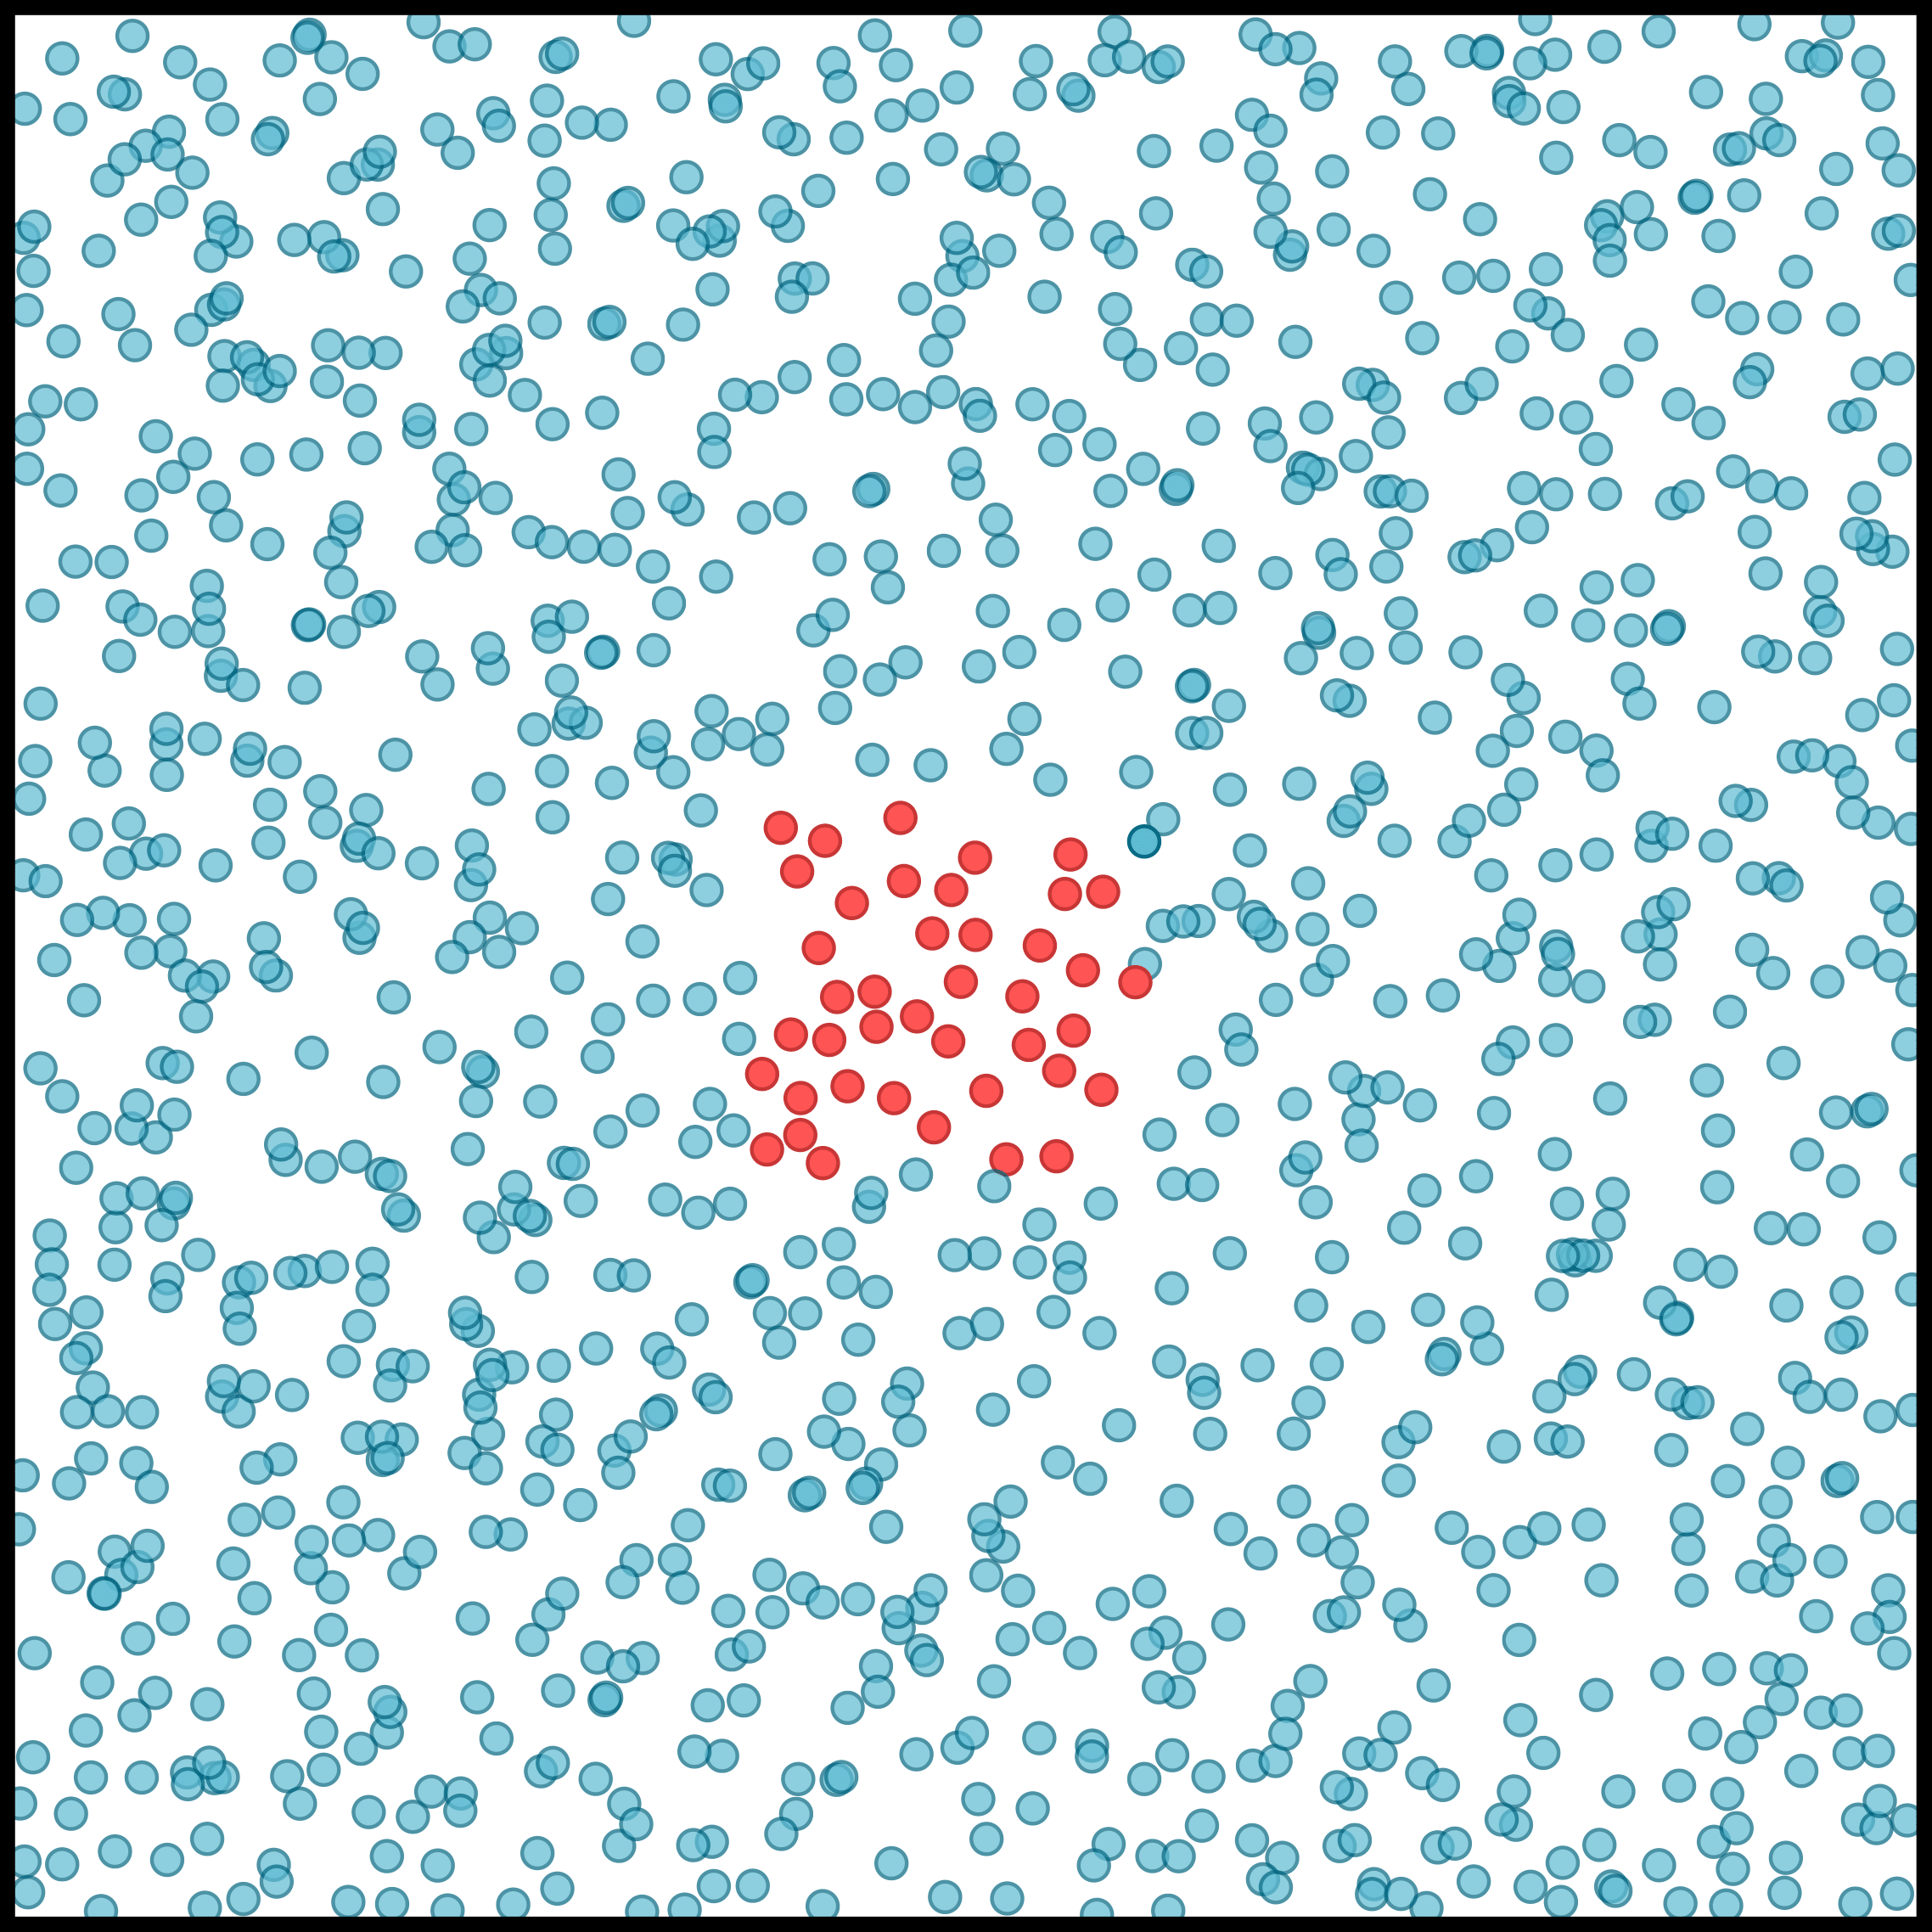
\includegraphics[width=.25\linewidth, angle=0]{figs/Introducao/Difusao_isotropica/water_molecule_t0.png}
    \label{fig::intro_difusao_isotropica_0}
    }
    \subfloat[Tempo = t]{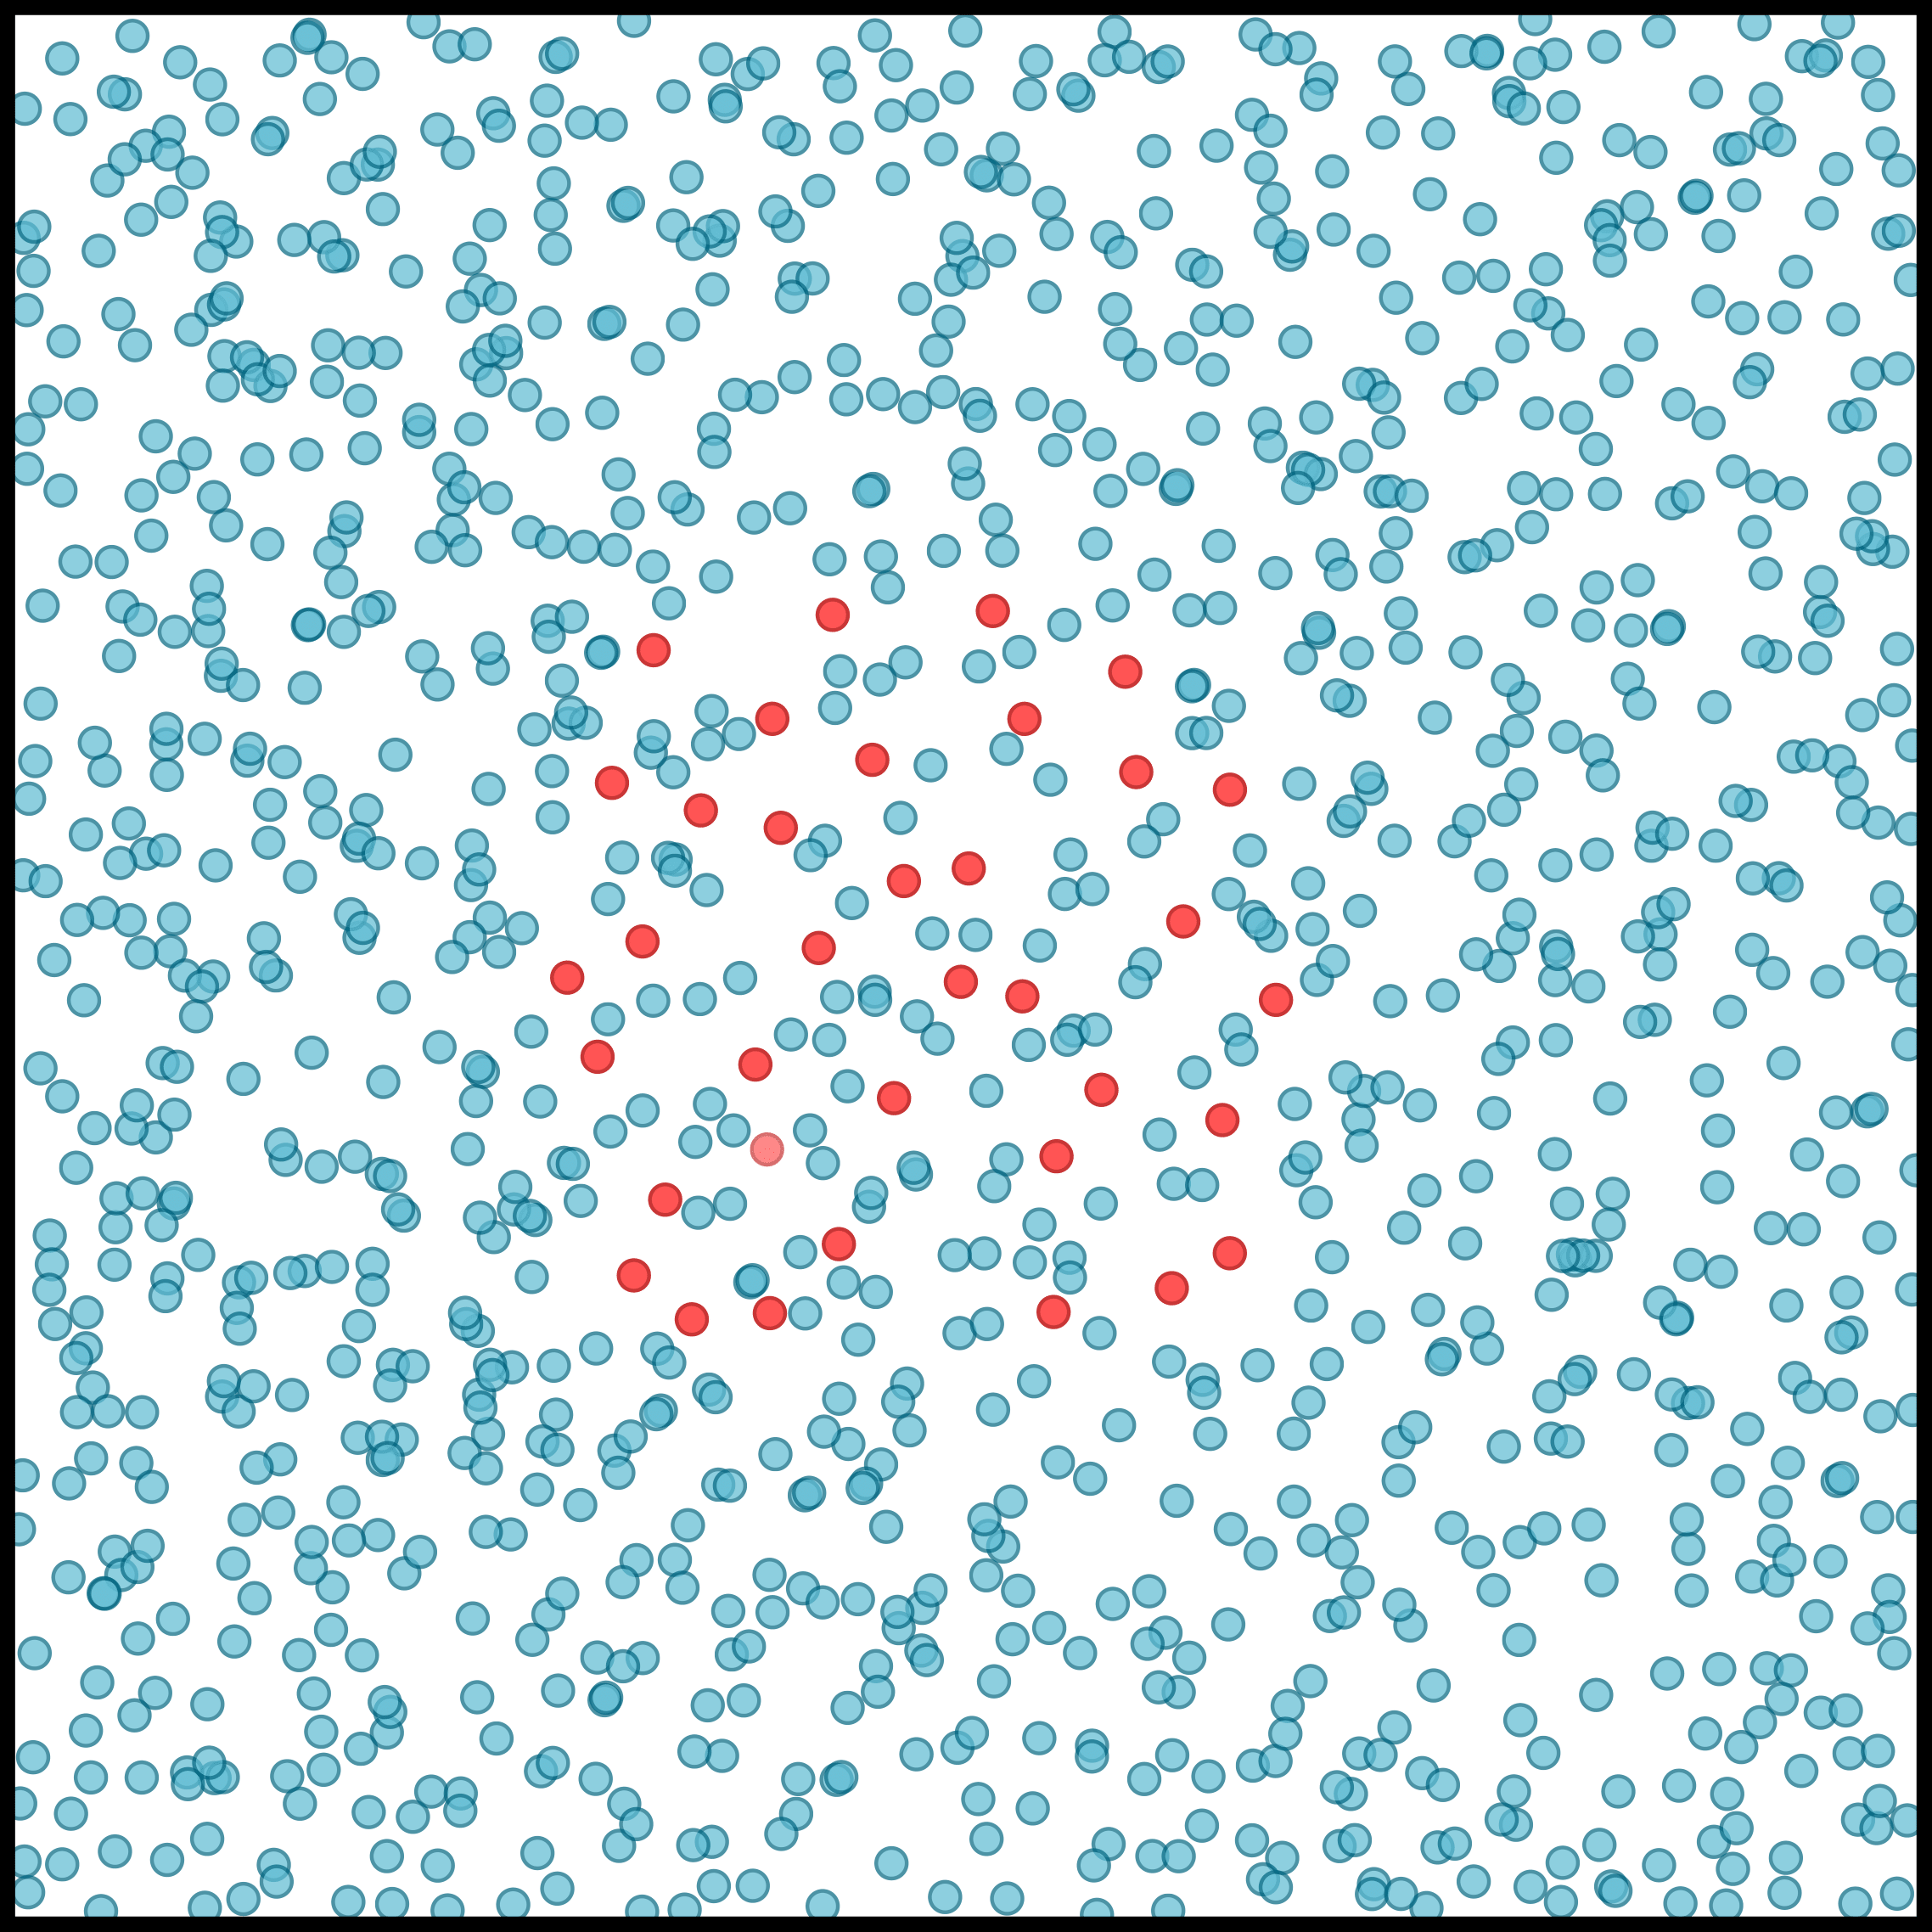
\includegraphics[width=.25\linewidth, angle=0]{figs/Introducao/Difusao_isotropica/water_molecule_t1.png}
    \label{fig::intro_difusao_isotropica_1}
    }
    \subfloat[Tempo = 2t]{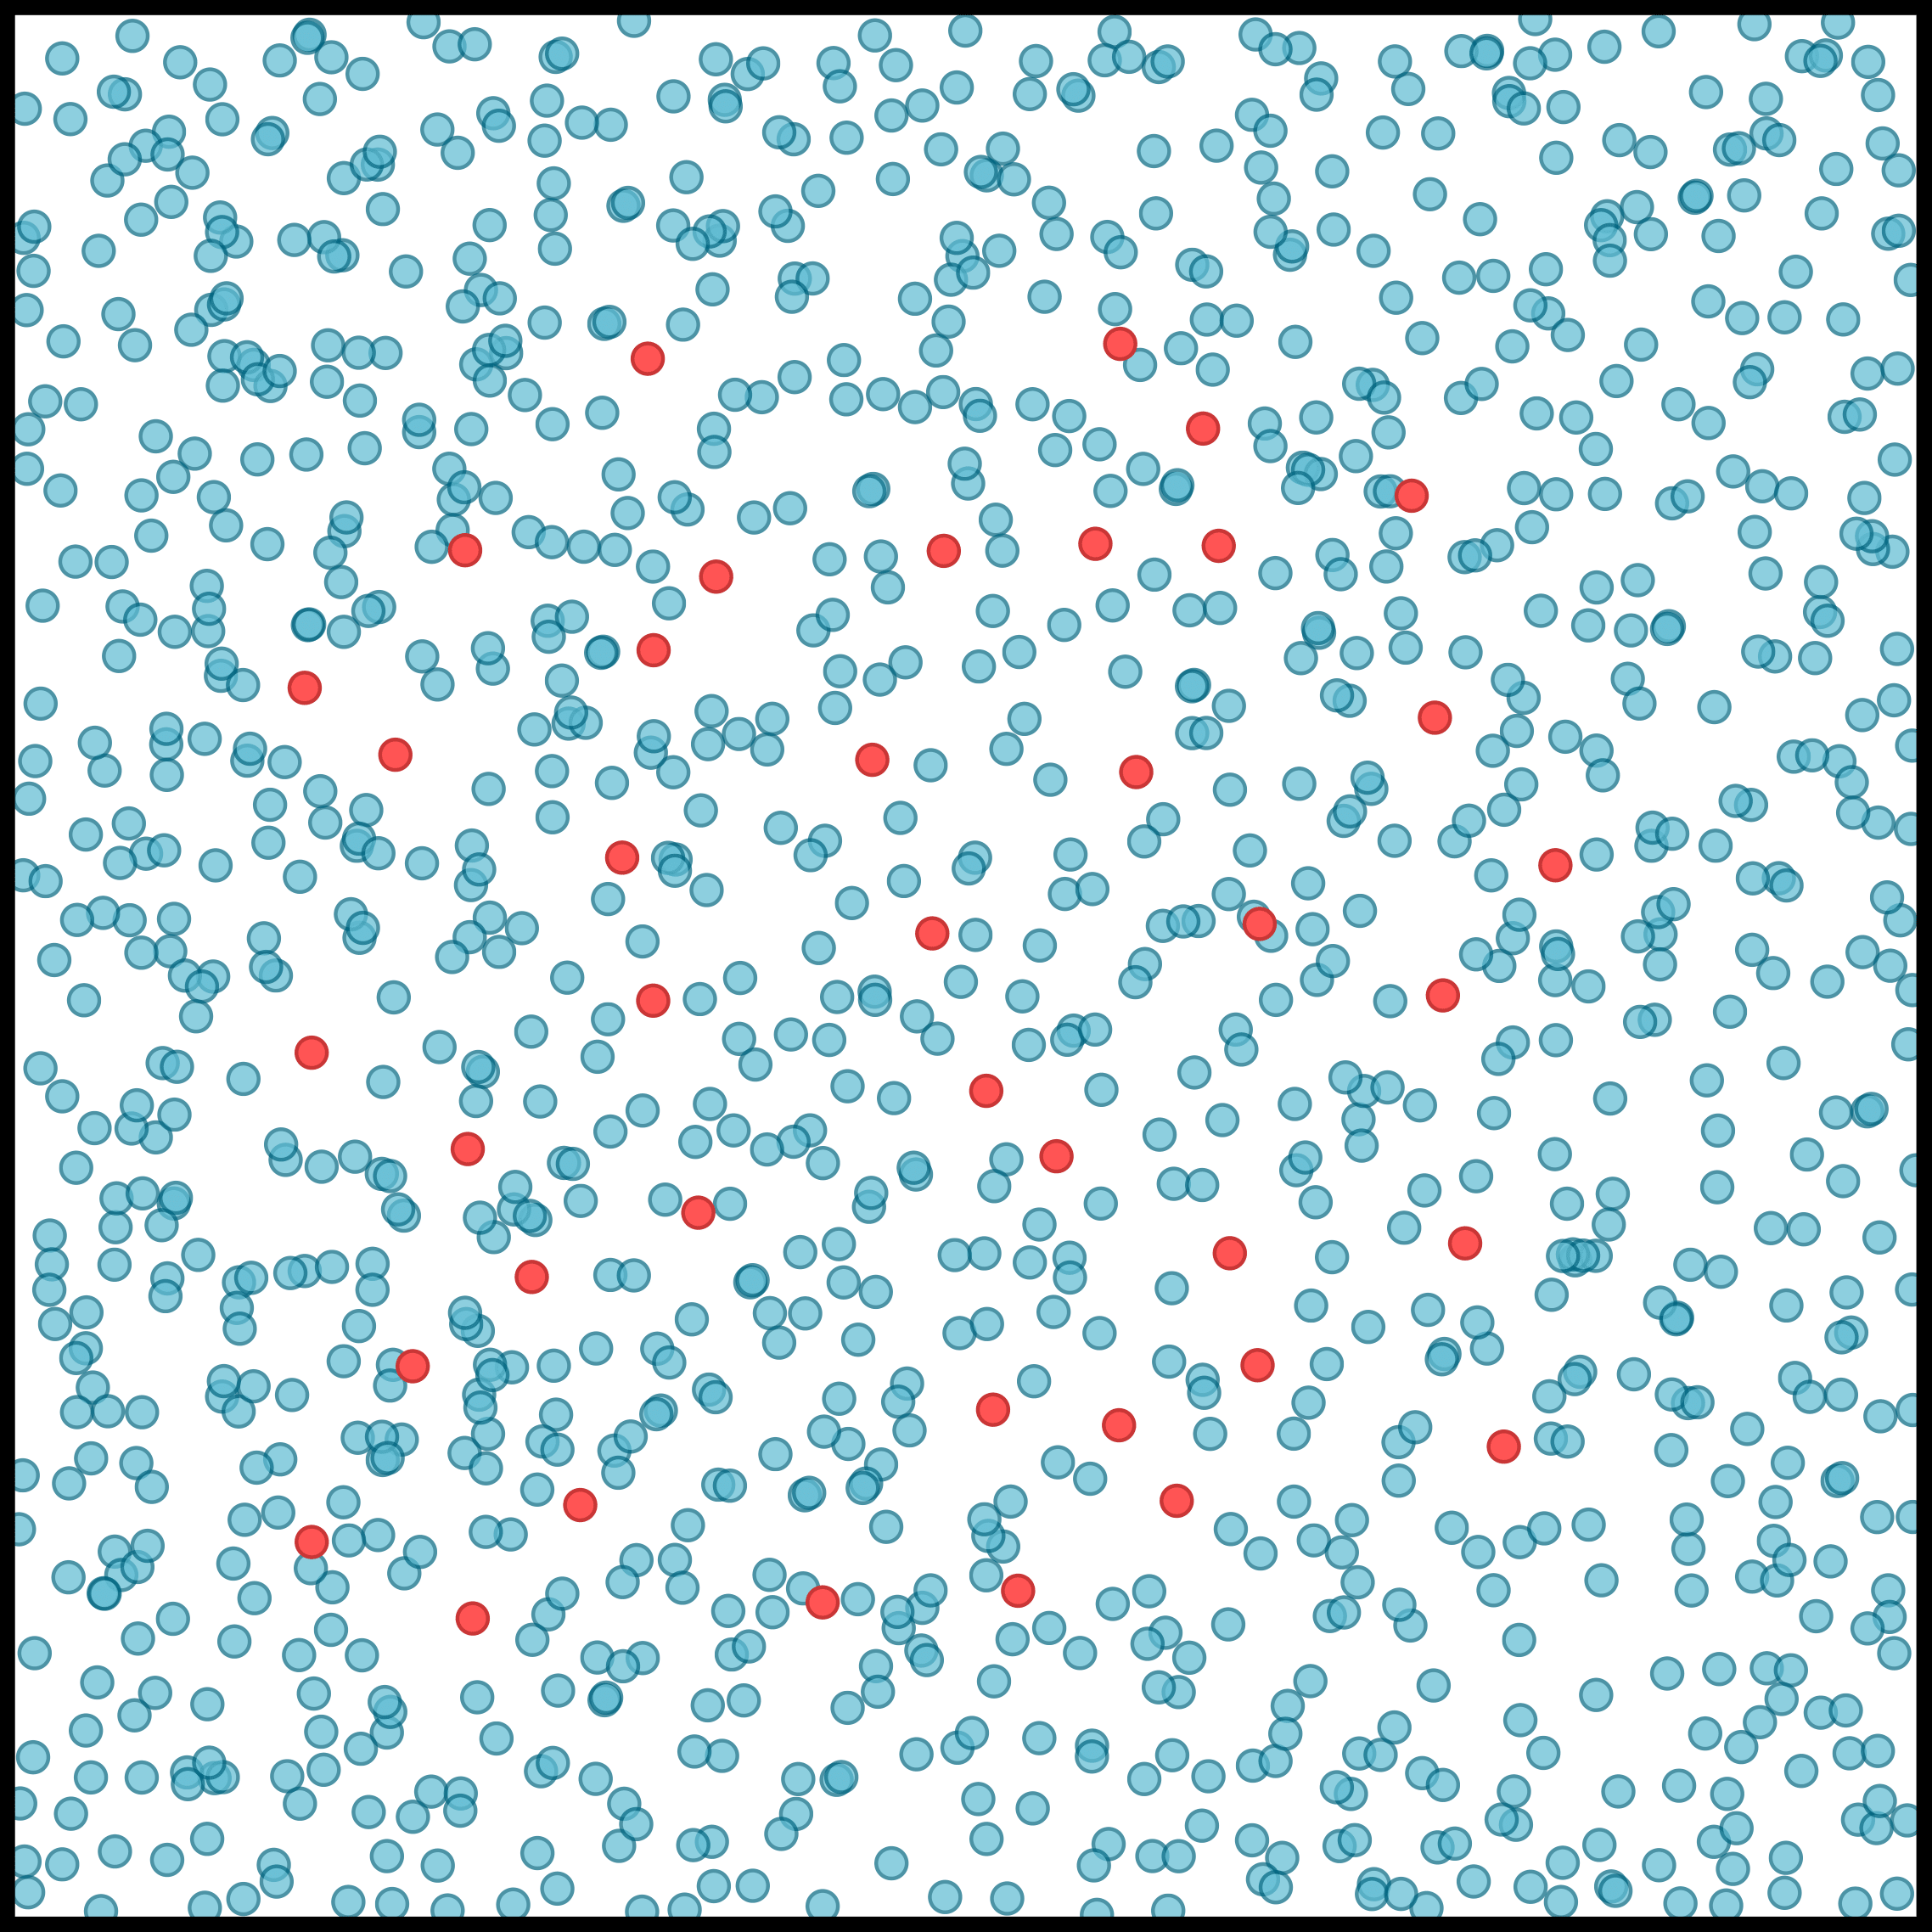
\includegraphics[width=.25\linewidth, angle=0]{figs/Introducao/Difusao_isotropica/water_molecule_t2.png}
    \label{fig::intro_difusao_isotropica_2}
    }
    \caption{Ilustração visual da difusão isotrópica. Os pontos azuis e vermelhos representam moléculas de fluidos. As moléculas em vermelho, inicialmente concentradas, se movimentam sem a escolha de uma direção preferencial. \\ Fonte: \cite{voltoline2016}}
    \label{fig::intro_difusao_isotropica}
\end{figure}

\begin{figure}[ht]
\centering
\captionsetup[subfloat]{farskip=0pt,nearskip=0pt}
    \subfloat[Tempo = 0]{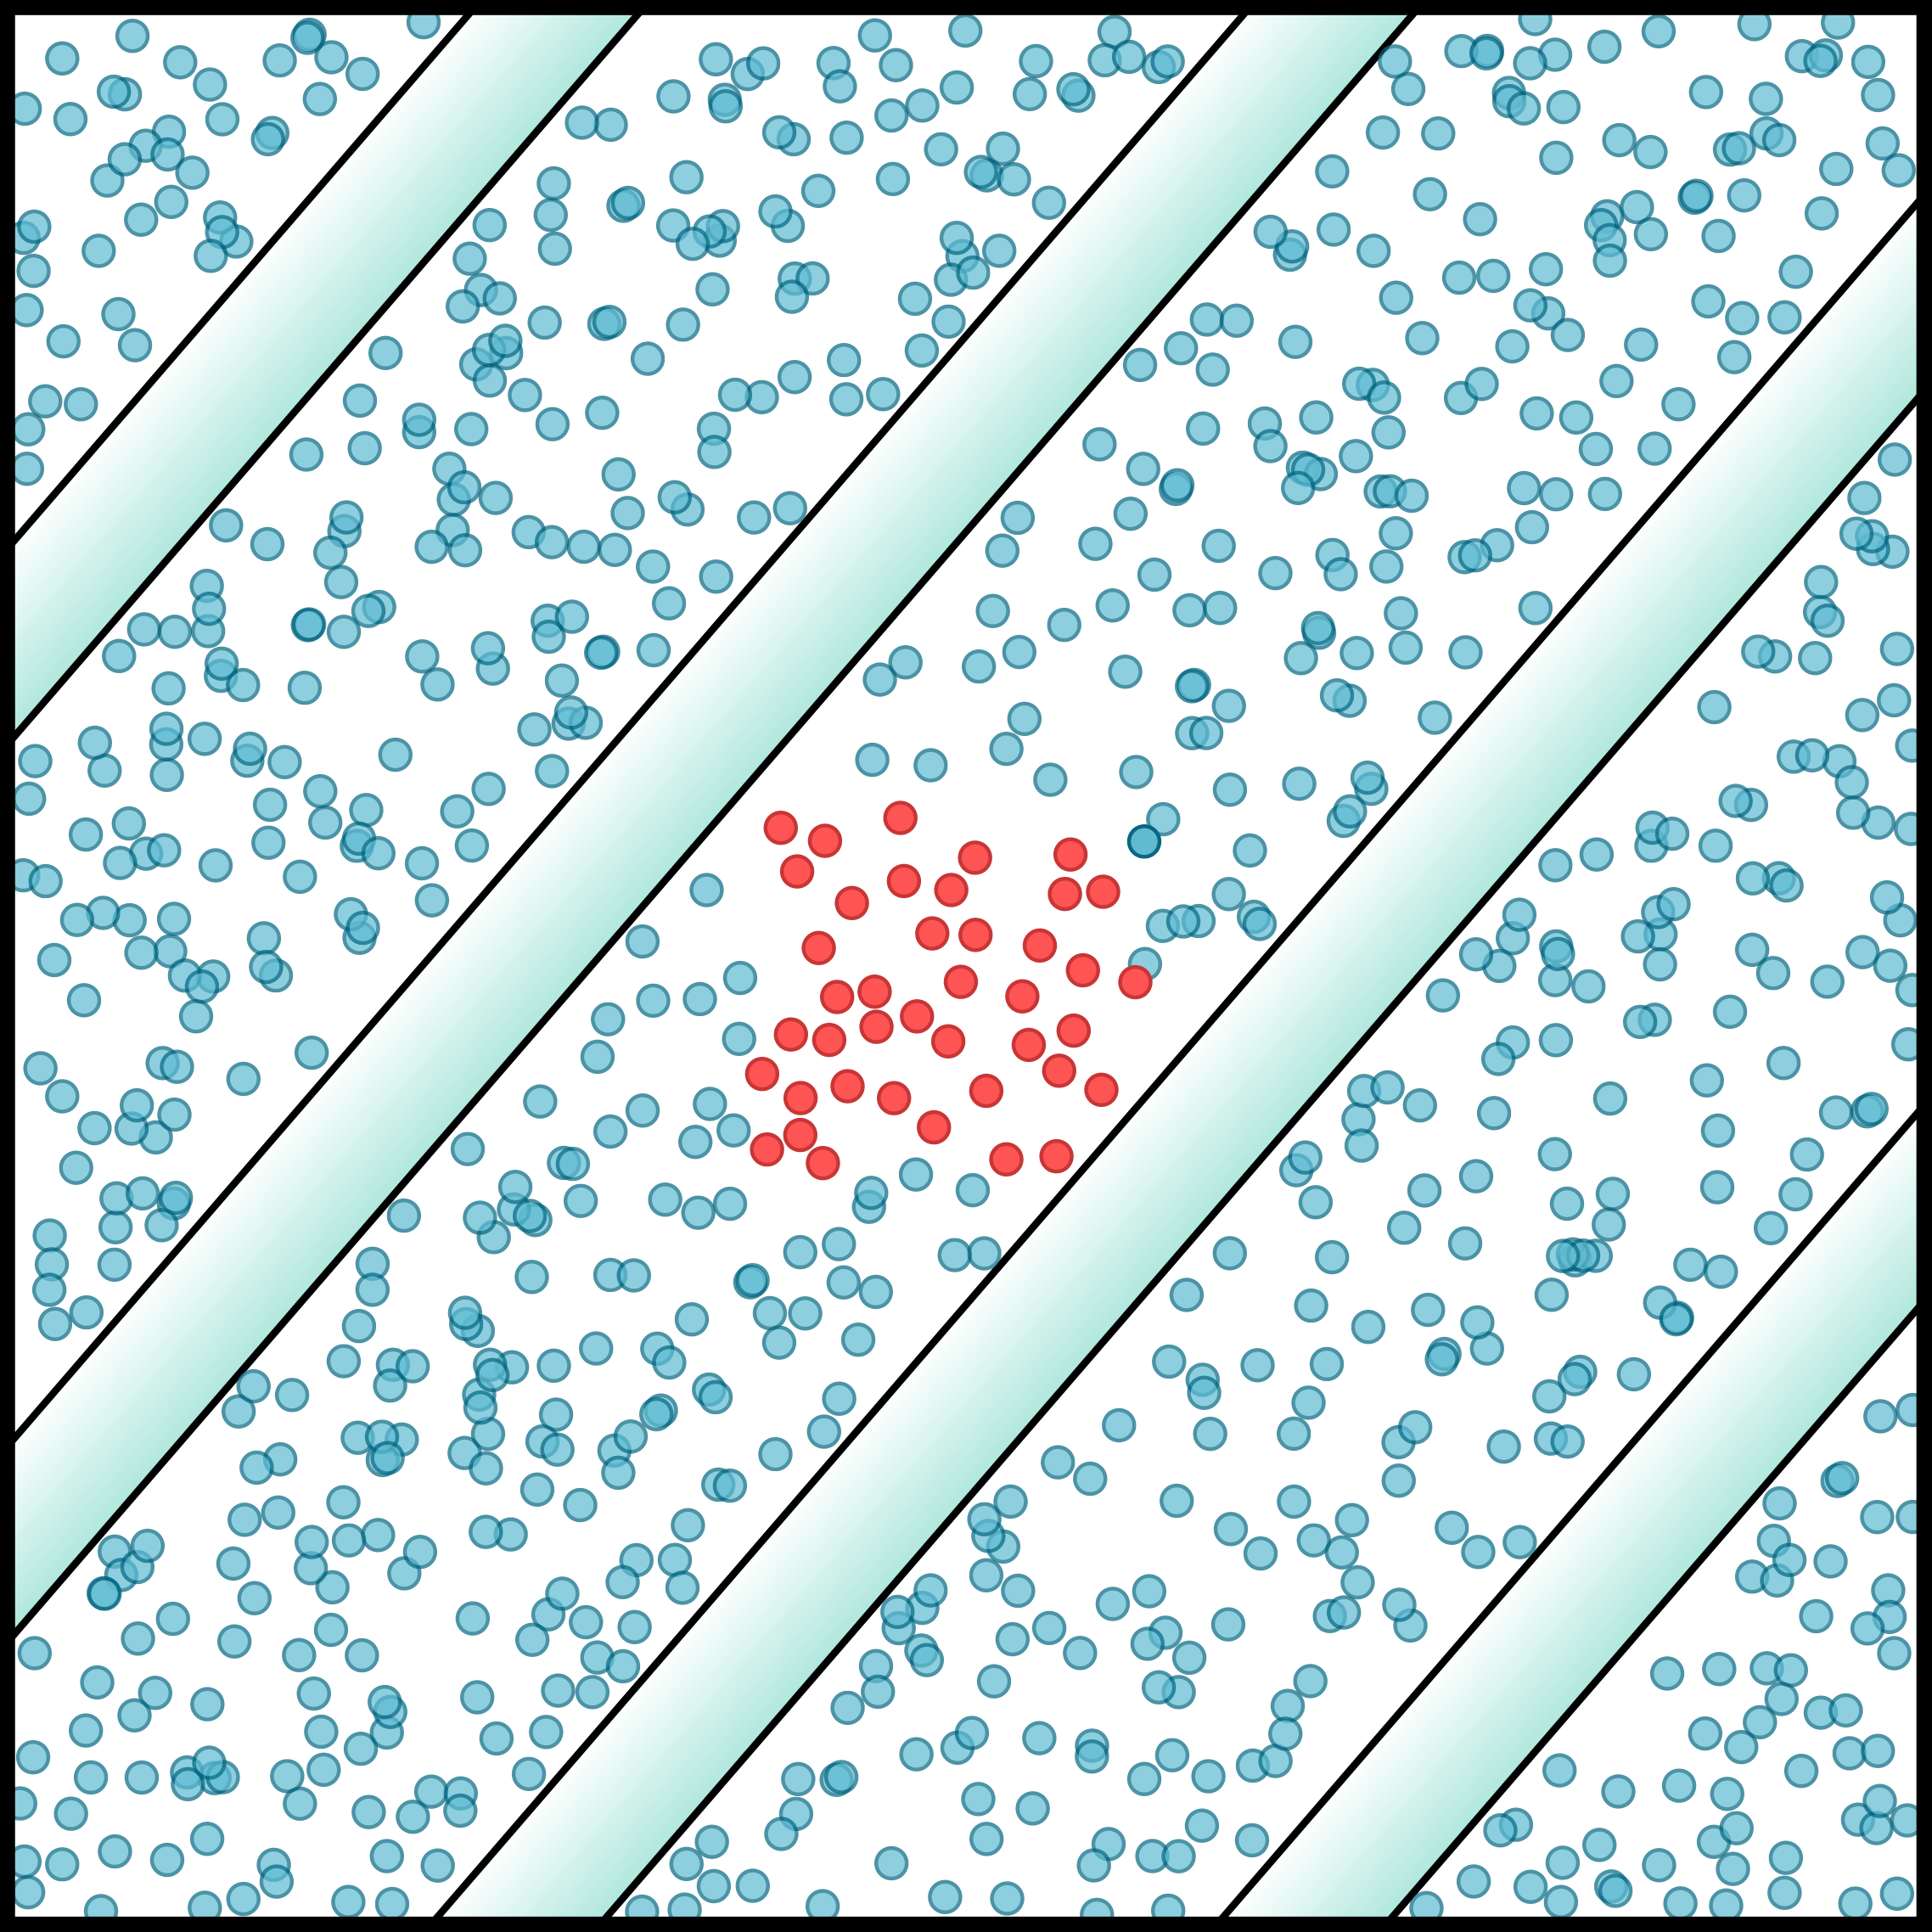
\includegraphics[width=.25\linewidth, angle=0]{figs/Introducao/Difusao_anisotropica/water_molecule_anisotropic_t0.png}
    \label{fig::intro_difusao_anisotropica_0}
    }
    \subfloat[Tempo = t]{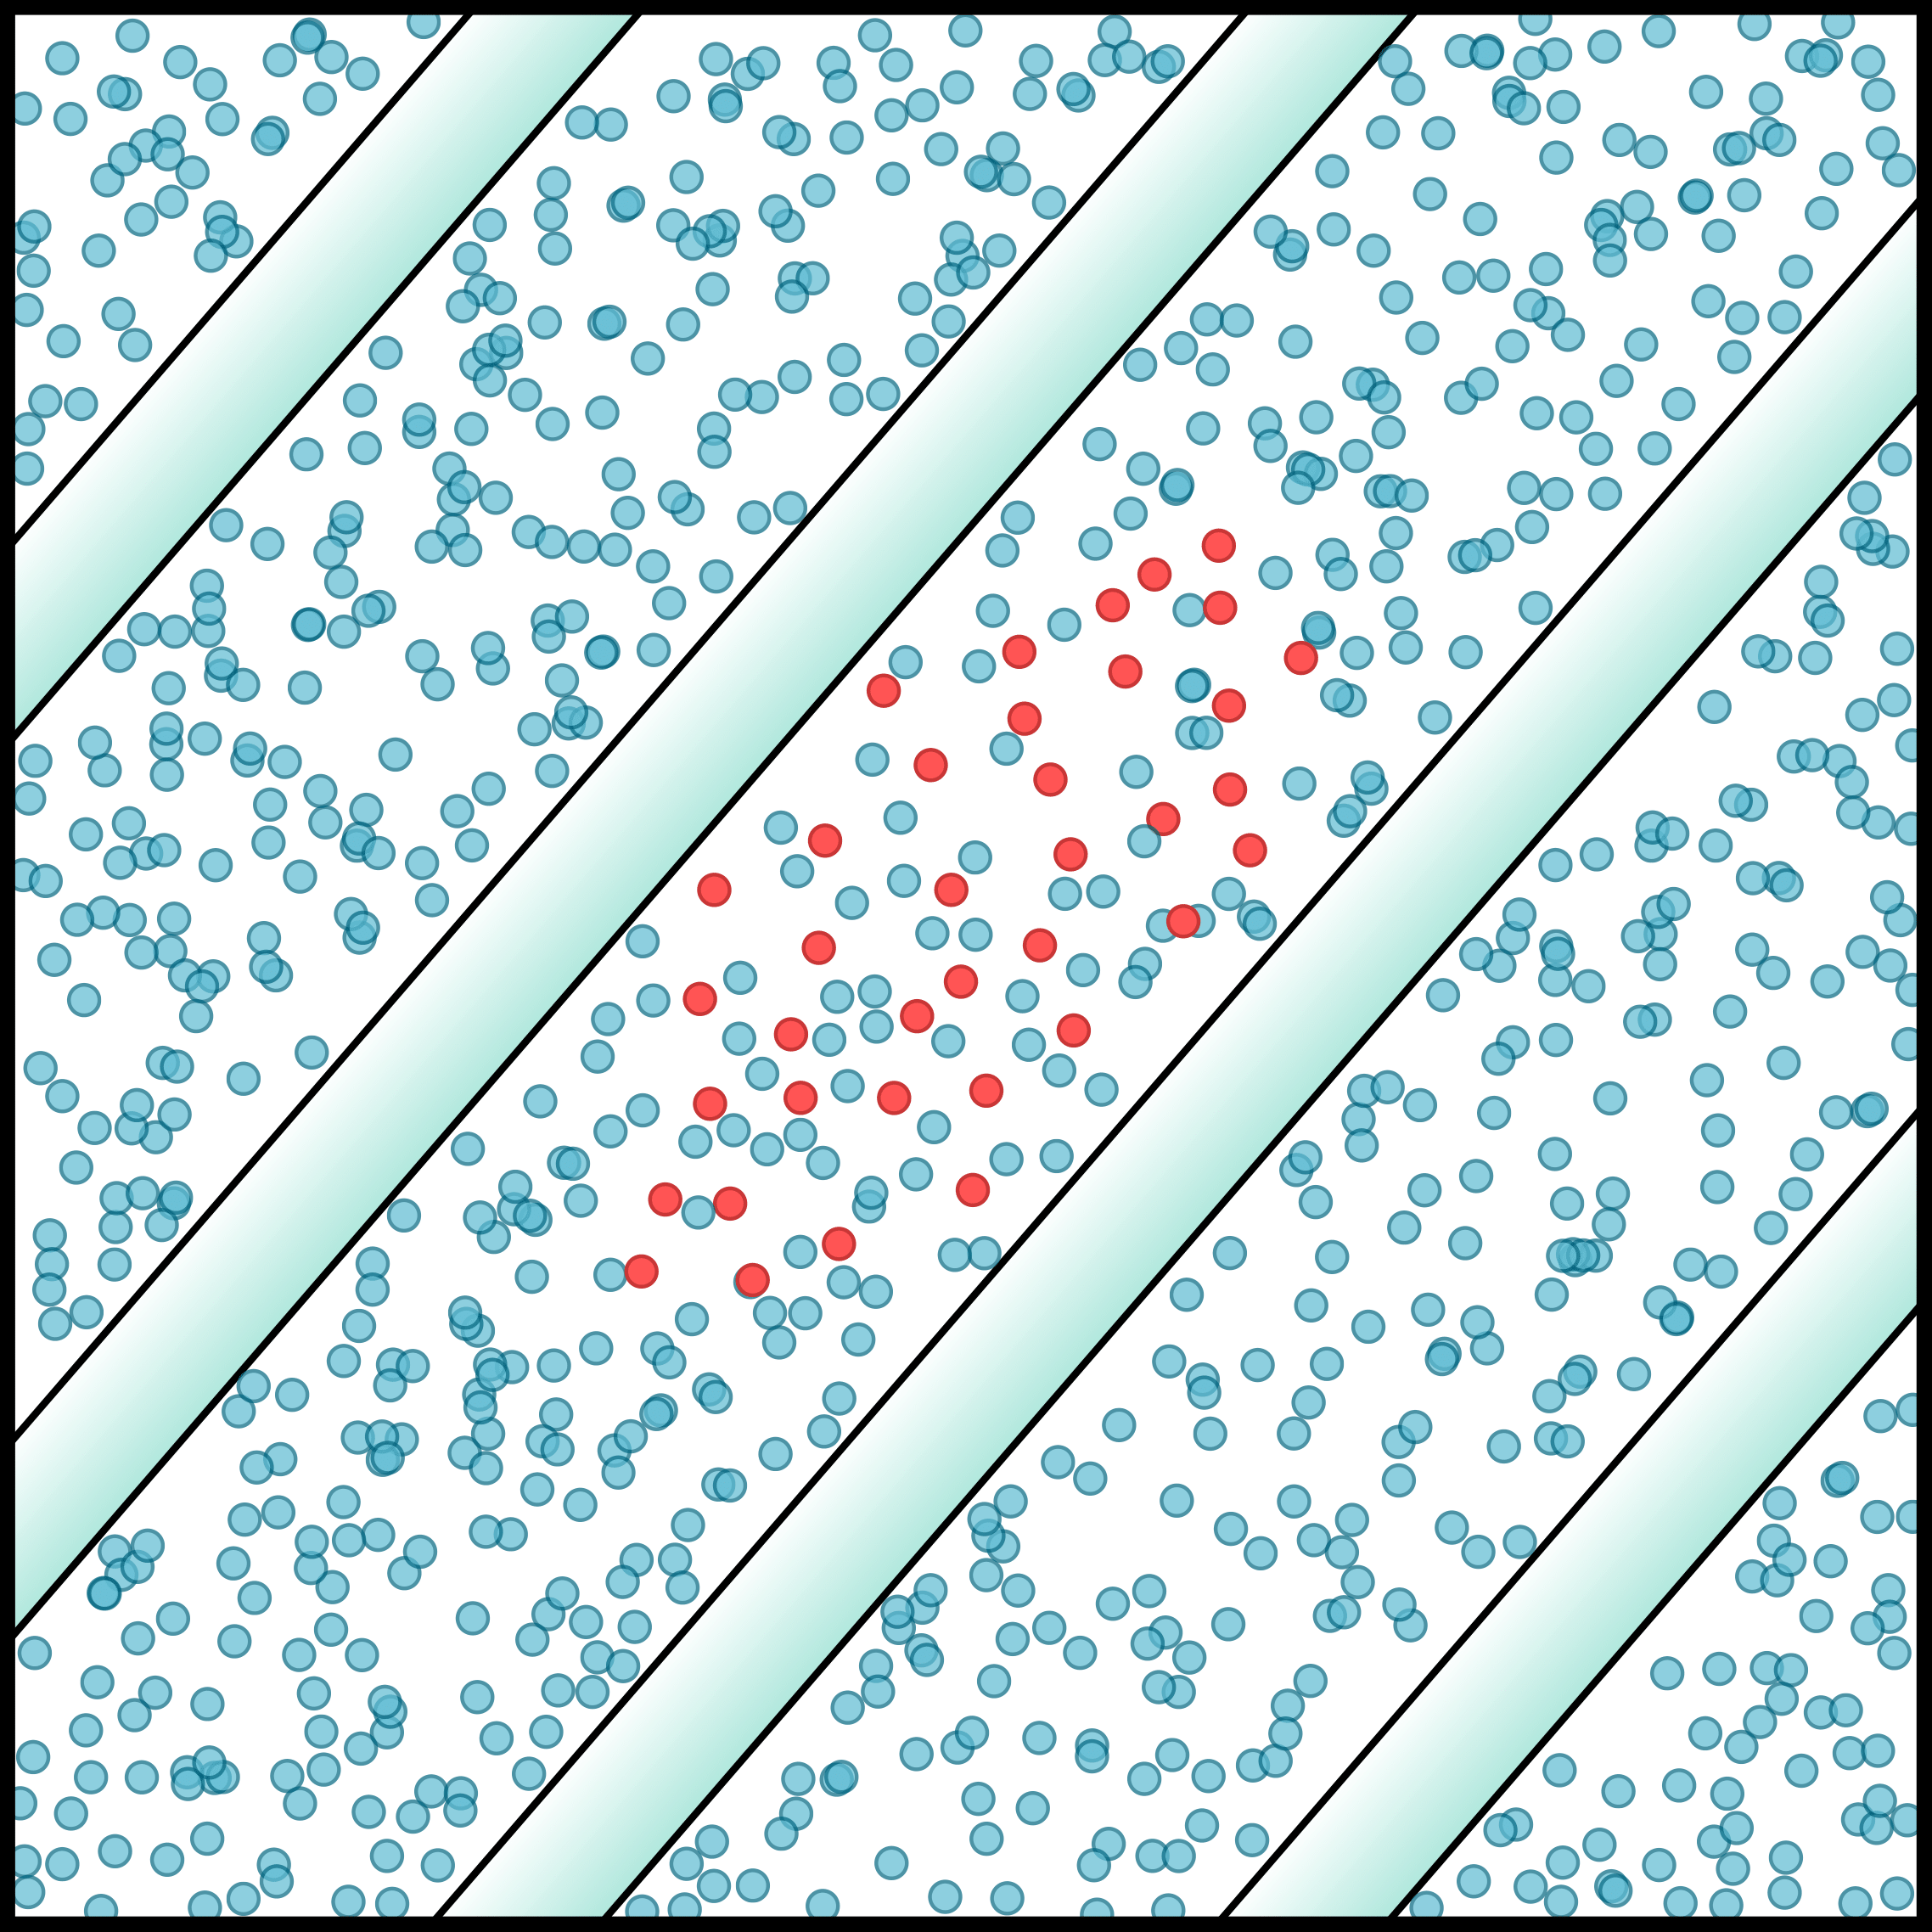
\includegraphics[width=.25\linewidth, angle=0]{figs/Introducao/Difusao_anisotropica/water_molecule_anisotropic_t1.png}
    \label{fig::intro_difusao_anisotropica_1}
    }
    \subfloat[Tempo = 2t]{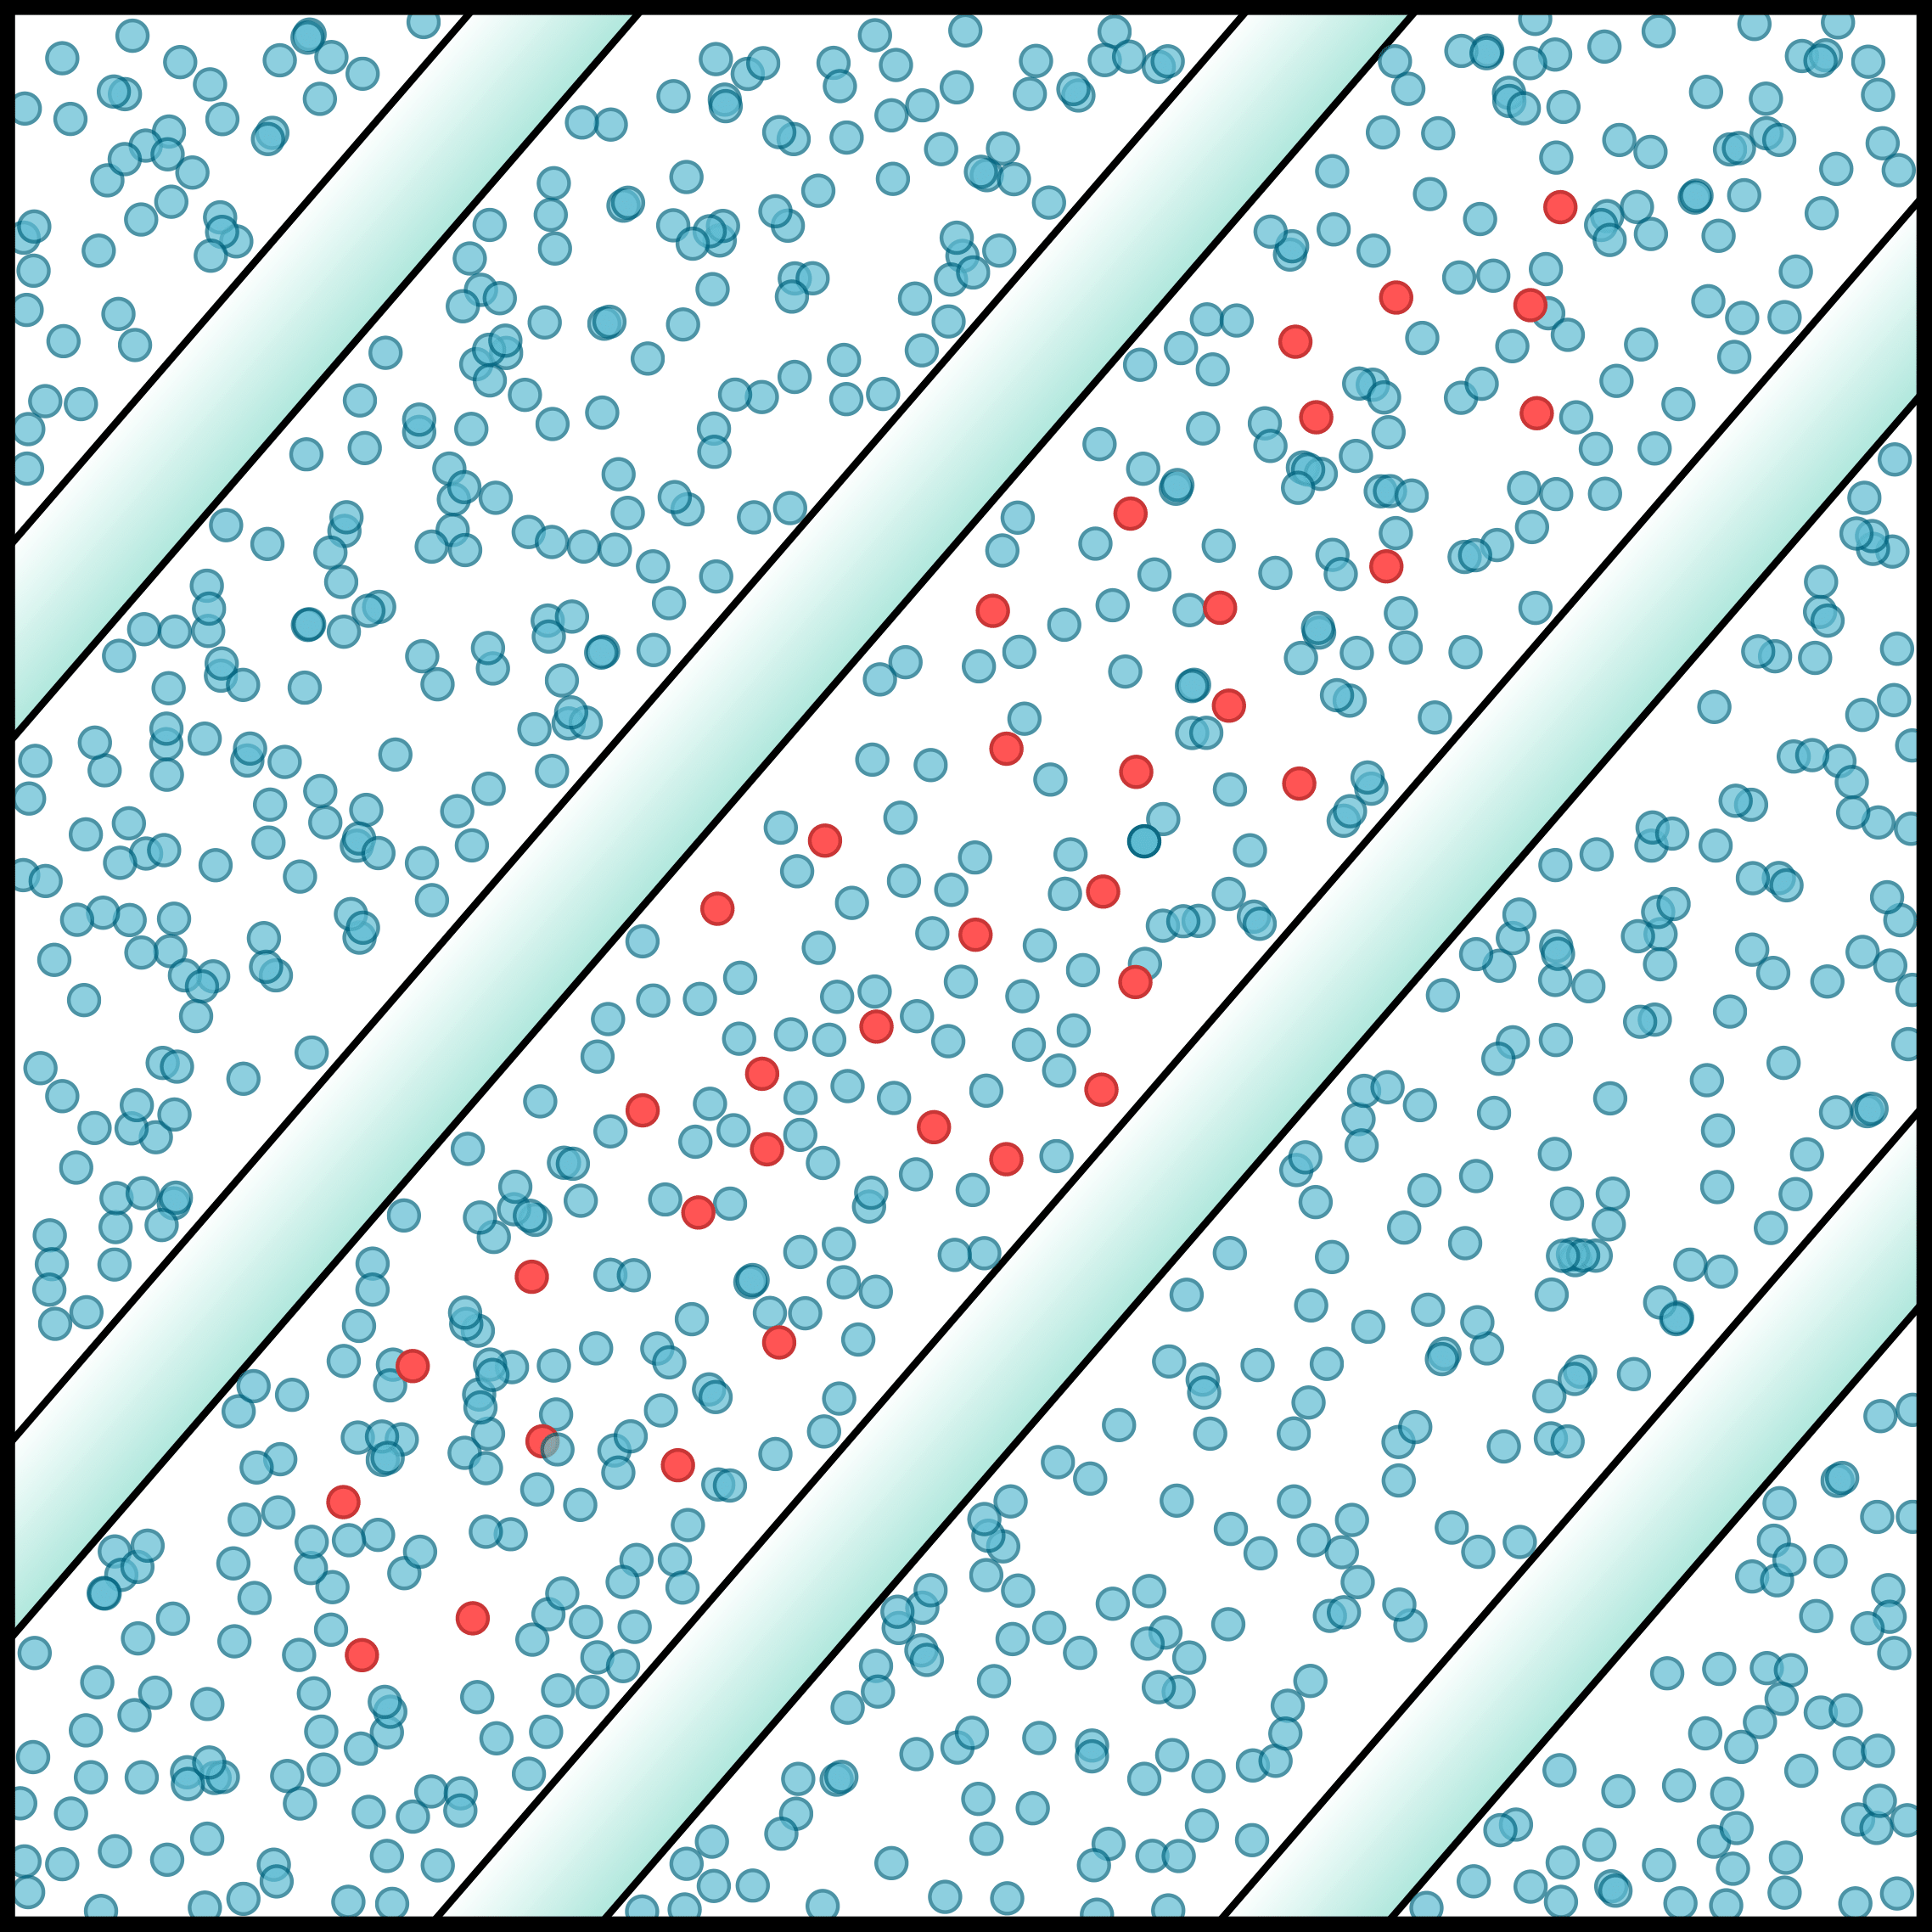
\includegraphics[width=.25\linewidth, angle=0]{figs/Introducao/Difusao_anisotropica/water_molecule_anisotropic_t2.png}
    \label{fig::intro_difusao_anisotropica_2}
    }
    \caption{Ilustração visual da difusão anisotrópica. Os pontos azuis e vermelhos representam moléculas de fluidos. As moléculas em vermelho, inicialmente concentradas, se movimentam de forma predominante em uma direção devido a restrição físicas em seu entorno. \\ Fonte: \cite{voltoline2016}
    }
    \label{fig::intro_difusao_anisotropica}
\end{figure}



%\todo{Por quê}
A medição das características difusão da água no cérebro pode fornecer informações sobre a matéria branca, que se referem a direção de fibras e conectividade do cérebro. Esta medição é possível através da ressonância magnética ponderada por difusão (\textit{diffusion-weighted magnetic resonance imaging} - DW-MRI ou DWI), que é o único meio não-invasivo a permitir tal informação. 



%O DWI é uma forma de ressonância magnética que gera contraste a partir da difusão das moléculas de água em determinadas direções \cite{DTI_Handbook}. %A partir do sinal adquirido, há ferramentas que  possibilitam o seu mapeamento em  fibras nervosas do cérebro humano \textit{in-vivo}.

%A ressonância magnética ponderada na sequência de difusão (\textit{diffusion-weighted magnetic resonance imaging} - DW-MRI ou DWI) é uma sequência de ressonância magnética que mensura a difusão das moléculas de água em determinadas direções \cite{DTI_Handbook}. A partir do sinal adquirido, há ferramentas que  possibilitam o seu mapeamento em  fibras nervosas do cérebro humano \textit{in-vivo}.

%!!A forma mais comum para gerar o DWI é através da sequência e pulsos PGSE (\textit{Pulsed Gradient Spin Echo}).


%Na aquisição do DWI, é escaneado um conjunto de volumes em que cada um possui a ponderação de único gradiente de difusão associado a um valor-b\footnote{O valor-b é uma métrica de sensitividade para difusão e é função de parâmetros da aquisição do DWI, como função da intensidade, duração e o intervalo de tempo dos gradientes de ponderação de difusão. Quanto maior o seu valor, maior o decaimento do sinal relativo à difusão.}, e, adicionalmente, um ou mais volumes sem ponderação de gradiente, denominado volume b0. A quantidade de volumes ponderados para diferentes direções de gradiente é denominada de resolução angular.

Há diversas técnicas para sumarizar os sinais coletados em informações de potenciais caminhos de fibras nervosas e que são objeto de pesquisa desde o início dos anos 90 \cite{descoteaux2015}. O método de imageamento mais amplamente utilizada para estes fins é chamada de imageamento por tensor de difusão (DTI - \textit{Diffusion Tensor Imaging}), proposto por \citeonline{Basser1994}. %\sout{há mais de 25 anos}\textcolor{red}{desde os primeiros trabalhos seminais ...}.

O DTI consiste em um mapeamento das amostras de difusão em um ponto contido em uma aquisição DWI em um modelo gaussiano, que é sintetizada por tensor de ordem 2, representado por uma matriz 3x3 simétrica. A informação referente ao processo de difusão é comumente extraída dos seus três autovetores e autovalores.

Há pesquisas na área de visualização em métodos de imageamento aplicados a aquisições DWI, tanto no que diz respeito à criação de glifos representativos do comportamento de difusão, quanto à reconstrução das fibras do cérebro -- denominada tractografia.

\citeonline{Basser1994} e \citeonline{Kindlmann2004}, por exemplo, propuseram glifos representativos que sintetizam a difusão a partir do DTI. A Fig. \ref{fig::intro_ex_DTI_glifos} ilustra glifos propostos por os glifos propostos por \citeonline{Kindlmann2004}, denominados superquádricos.

As fibras reconstruídas consistem de informações direcionais extraídas de um método de imageamento e costumam ser representadas por linhas, como ilustrado na Fig. \ref{fig::intro_ex_DTI_tractografia}. Algoritmos de tractografia baseados em DTI são exemplificados por \citeonline{Weinstein1999} e \citeonline{basser2000}. 

\begin{figure}[ht]
\captionsetup[subfloat]{farskip=0pt,nearskip=0pt}
    \subfloat[Tensores de difusão representado por glifos superquádricos em uma fatia axial do cérebro na região do corpo caloso. As cores representam a direção predominante de difusão onde vermelho é esquerda-direita, azul é superior-inferior e verde é anterior-posterior]{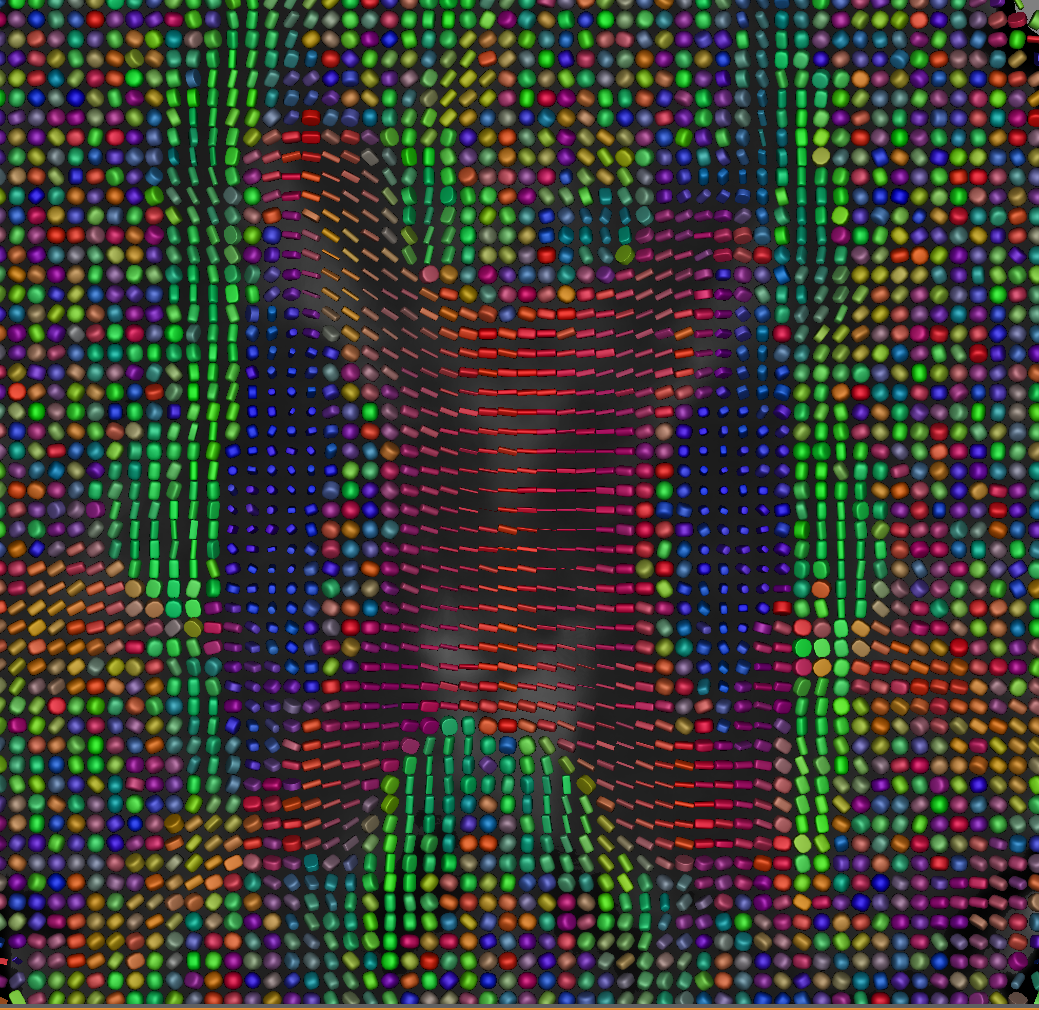
\includegraphics[width=.52\linewidth, angle=0]{figs/Introducao/ex_DTI_Superquadrica.png}
    \label{fig::intro_ex_DTI_glifos}}
    \hfill
    \subfloat[Trato fascículo inferior fronto-occipital (IFOF). A cor predominantemente verde indica sua trajetória, que ocorre na direção anterior-posterior. As linhas são reconstruídas com base no proposto por \citeonline{Weinstein1999} ]{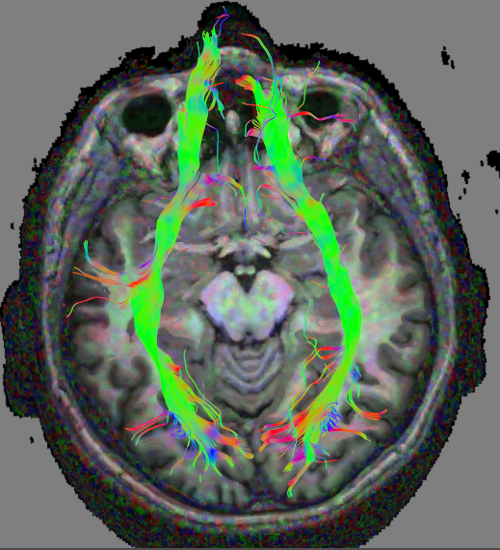
\includegraphics[width=.46\linewidth, angle=0]{figs/Introducao/ex_DTI_tractography.png}
    \label{fig::intro_ex_DTI_tractografia}}
    \caption{Ilustração de resultados de pesquisa na área de visualização em ressonância magnética de difusão utilizando o DTI.}
    \label{fig::intro_ex_DTI}
\end{figure}



A partir da visualização de dados extraídos dos tensores, há estudos que buscam inferir sobre a substância branca e utilizá-las em diferentes estudos e diagnósticos. Como alguns exemplos, temos:

\begin{itemize}
    \item evidência de correlações de métricas do DTI com a degeneração do cérebro causada pela esclerose lateral amiotrófica e o seu potencial uso como biomarcador \cite{cirillo2012, baek2020};
    \item diagnósticos de isquemia cerebral aguda em estágios iniciais, o que não é possível com MRI convencionais \cite{dong2004};
    \item aplicação de métricas e tractografia à redes cognitivas na epilepsia do lobo temporal \cite{leyden2015}
\end{itemize}

Devido a sua natureza de modelagem, o DTI apresenta limitações. O modelo gaussiano descreve bem regiões de fibras em que o comportamento de difusão ocorre predominantemente em uma direção. Em pontos que contém múltiplas fibras e que estão dispostas nas mais variadas configurações (por exemplo: cruzamento, bifurcação, mistura, "beijo") o modelo gaussiano não sintetiza de forma correta o comportamento da difusão, impedindo o cômputo das direções plausíveis para reconstrução de uma fibra de interesse \cite{fillard2011, daducci2014}. Há uma estimativa que entre 66\% a 90\% da substância branca do cérebro contém múltiplas configurações de cruzamento de fibra \cite{descoteaux2015} e a limitação do DTI é um obstáculo para traçar o caminho de fibras do cérebro de forma efetiva.

Cientes das limitações do DTI, pesquisadores da área propuseram métodos de imageamento com modelos matemáticos mais avançados e descritivos do processo de difusão, os quais passaram a demandar aquisições de mais amostras de sinais de difusão em comparação as aquisições utilizadas para o DTI, tais aquisições são denominadas imagem de difusão por alta resolução angular  (HARDI - \textit{High Angular Resolution Diffusion Imaging}). A tese de doutorado de David Tuch \cite{tuch2002} é o trabalho seminal da área.




%  do tensor de difusão representam três direções ortogonais cujos respectivos autovalores representam a magnitude de difusão, que são máximos para restrição de ortogonalidade.

%\todo[inline]{Abstraindo o que você escreveu ... há duas linhas de empenho: visualização dos sinais de difusão por amostra (modelagem local da geometria das fibras) e/ou por fibra (modelagem global da conectividade das amostras). É melhor colocar Fig 1.1 e 1.2 uma ao lado da outra. Facilita análise comparativa.}








%\begin{figure}[ht]
%
%\centering
%\includegraphics[width=.485\linewidth, %angle=00]{figs/Introducao/ex_DTI_Superquadric%a.png}
%\centering
%\caption{Tensor de difusão representado por %glifos superquádricos em uma fatia axial do %cérebro na região do corpo caloso. As cores %representam a direção predominante de difusão %onde vermelho é esquerda-direita, azul é %superior-inferior e verde é %anterior-posterior}
%\label{fig::intro_ex_DTI_Superquadrica}
%\end{figure}

%\begin{figure}[ht]
%\centering
%\includegraphics[width=.485\linewidth, %angle=00]{figs/Introducao/ex_DTI_tractography%.png}
%\caption{Trato fascículo inferior %fronto-occipital (IFOF). A cor %predominantemente verde indica sua %trajetória, que ocorre na direção %anterior-posterior}
%\label{fig::intro_ex_DTI_Tractografia}
%\hfill
%\end{figure}




%\section{Motivação}
%\label{ssec:motivation}



%Uma aquisição DWI é considerada HARDI se há 45 ou mais gradientes de ponderação de difusão. Esta modalidade de aquisição se diferencia de uma aquisição DTI, que costuma possuir entre 6 a 32 direções \cite{descoteaux2015}.


%\todo{\url{https://www.researchgate.net/figure/Sampling-schemes-in-q-space-a-Cartesian-sampling-dedicated-to-diffusion-spectrum_fig3_319558026}}.

Durante a década de 2000, foram propostos métodos de imageamento mais descritivos do processo de difusão que o DTI, que podem ser exemplificados nos trabalhos: \cite{tuch2002}, \cite{TuchQBall2004}, \cite{tournier2007}, \cite{wedeen2005} e \cite{yeh2010}. Estes métodos tinham como objetivo principal resolver o problema o cruzamento de fibras, assim superando as limitações do DTI. Para diferenciá-los do DTI, neste trabalho chamaremos estes métodos de imageamento de \textbf{métodos HARDI}.

%Durante a década de 2000, foram propostos métodos de imageamento mais descritivos do processo de difusão que o DTI . Alguns deles consistem na abordagem multi-tensor \cite{tuch2002}, o \textit{Q-Ball Imaging} (QBI) \cite{tuch2002, Kindlmann2004}, \textit{constrained spherical deconvolution} (CSD) \cite{tournier2007}, \textit{diffusion spectrum imaging} (DSI) \cite{tuch2002,wedeen2005} e a amostragem generalizada do espaço Q (GQI - \textit{generalized Q-space sampling}) \cite{yeh2010}.  no qual padrões de fibras subjacentes podem ser inferidos. Para diferenciá-los do DTI, neste trabalho chamaremos estes métodos de imageamento de \textbf{métodos HARDI}.

%Uma ODF, no contexto de DWI, consiste em uma função que associa um conjunto de direções a um valor escalar de difusividade. A representação em forma de glifos para ODFs geralmente consistem na plotagem polar esférica (\textit{spherical polar plot}) de uma ODF min-max normalizada no intervalo [0, 1] \cite{TuchQBall2004}, conforme mostrado na Fig. \ref{fig::ex_glifo_hardi}. Chamaremos esta categoria de glifos neste trabalho de \textbf{glifos ODF}. A renderização interativa desses glifos é um ponto principal deste trabalho e os trabalhos de \citeonline{shattuck2008} e \citeonline{peeters2009, almsick2011} trazem diferentes abordagens para este fim.

%\begin{figure}[h]
%   \centering
%       \addtolength{\leftskip} {-2cm} % increase (absolute) value if needed
%    \addtolength{\rightskip}{-2cm}
%
%    %\vspace*{3mm}
%    \centering
%    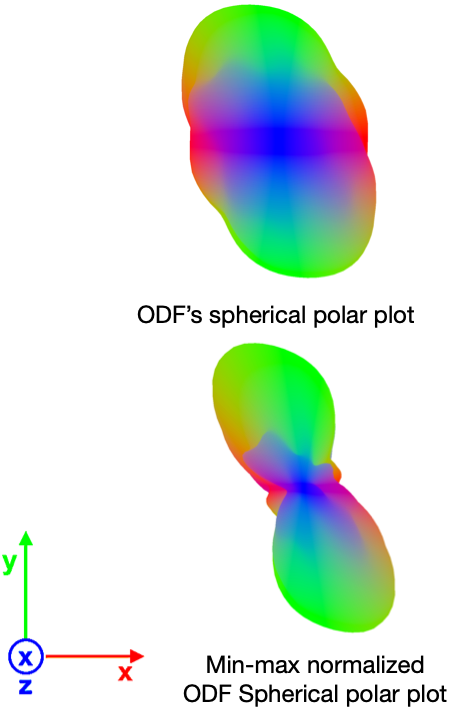
\includegraphics[width=.35\linewidth, angle=0]{figs/Introducao/SphericalMeshModulation.png}
%   \caption{Plotagem polar esférica de uma ODF e sua versão min-max normalizada. A normalização enfatiza a direção dominante de difusão. As cores representam a direção no espaço da superfície, onde o vermelho representa horizontal; verde, a vertical; e azul a direção normal ao plano da tela.}
%    \label{fig::ex_glifo_hardi}
%\end{figure}
Os métodos definem transformadas que são aplicadas nas amostras dos sinais de difusão em cada \textit{voxel} em uma função, na qual a distribuição de direções de fibra subjacentes podem ser inferidas. A extração geralmente é feita através da detecção de máximos locais destas funções, nos quais, se aplicados sobre aquisições com uma relação sinal ruído razoável, tendem a modelar bem esta distribuição \cite{fillard2011}.

A partir da extração de direções subjacentes de fibras, tem sido possível gerar algoritmos de tractografia mais coerentes com os tratos reais e que levem em consideração mais nuances do sinal de difusão que o DTI, especialmente em regiões que contém as mais diversas configurações de múltiplas de fibras. Alguns trabalhos que trazem evidências da melhoria de tractografia utilizando métodos HARDI, podem ser exemplificados por:

\begin{itemize}
    \item \citeonline{berman2009} evidencia a melhor reconstrução da conectividade no trato motor na presença de tumor;
    \item \citeonline{bucci2013} evidencia um melhor delineamento do trato corticoespinhal utilizando um método HARDI comparado ao DTI, tendo o validado com estimulação cortical;
    \item \citeonline{kuhnt2013} documenta a melhora da tractografia das radiações ópticas utilizando HARDI em pacientes com glioma;
\end{itemize}
Mesmo com estas evidências, aquisições e métodos HARDI não são popularmente utilizadas clinicamente.


%A partir das ODFs, a direção local de fibras em um \textit{voxel} é modelada de forma adequada pela extração de seus máximos locais \cite{fillard2011}, sendo assim a base para algoritmos de tractografia.  %\textcolor{red}{Porém, (comentar o que falta ainda para popularizar o seu uso clínico em relação a DTI) ...}

No uso clínico, o DTI é ainda muito mais utilizado que métodos HARDI \cite{descoteaux2015}. As vantagens do DTI se referem a sua aquisição, que requer uma quantidade de dados menor, implicando em um menor tempo para ser feita, e a popularidade de aplicativos que processam DWI por este método de imageamento. Adicionalmente, O DTI demanda uma menor quantidade memória para armazenar parâmetros intrínsecos ao seu método comparados aos métodos HARDI e, geralmente o cômputo de parâmetros relacionados em diferentes aplicações, como o próprio cômputo do método, renderização de glifos e tractografia, são computacionalmente menos exigentes.

%Falar de tratos que HARDI resolve e DTI não?

%Em tractografia, tanto baseada em DTI, quanto HARDI, há avanços no entendimento de patologias, como esclerose múltipla, mal de Parkinson, esquizofrenia e derrame \cite{SCHILLING2019194}, e mesmo com essas aplicabilidades, há muitos desafios na área.

%Embora os máximos de ODF obtidas através de métodos HARDI consigam resolver os problemas que dizem respeito à estimativa de direções de fibras de forma local, os métodos não inferem sobre a configuração de fibras -- por exemplo, se as diferentes fibras se cruzam ou se "beijam" \cite{SCHILLING2019194}. A busca por informações adicionais para inferir a natureza da configuração entre múltiplas fibras em diferentes regiões é uma oportunidade ainda em aberto.

%%RELER O ARTIGO DO SCHILING E MOSTRAR OPORTUNIDADES 



%\todo[inline]{Sugiro mencionar aqui o artigo de Schilling et al. mostrando os desafios ainda em aberto.}

\section{Motivação}
\label{ssec:motivation}

Nosso grupo de pesquisa tem a intenção de fazer um ambiente exploratório para volumes de difusão para volumes de difusão através de um método HARDI. Neste ambiente, um especialista tem total liberdade para construção e análise de forma não invasiva de fibras e para este fim, desenvolveremos um sistema de visualização interativa de perfis de difusão gerados pelo método de imageamento utilizado em glifos e um algoritmo de tractografia interativo, como ilustrado na fluxograma da Fig. \ref{fig::flowchart_vmtk_hardi}.

Diante destes desafios em aberto, este trabalho aborda a implementação de uma método HARDI para processamento de volumes de difusão e a proposição de um algoritmo para renderização interativa de glifos que sintetizem as funções obtidas através destes métodos. Este algoritmo é integrado ao ambiente de visualização multimodal desenvolvido e publicado por \citeonline{voltoline2021}.

%O sistema tem a intenção de ser usado por um especialista para que a partir de um DWI, ele possa construir e analisar de forma não invasiva fibras dos cérebros a partir de um método. Para este fim, 

A visualização interativa de perfis de difusão em cada amostra dá ao especialista uma visão de como o método utilizado o reconstrói a partir do sinal de difusão. A partir dele, pode-se inferir visualmente sobre o método de imageamento utilizado quanto a sua adequabilidade para com a aquisição utilizada. Adicionalmente, há evidências que o uso de glifos superquádricos posicionados em seus respectivos \textit{voxels} em um ambiente de exploração interativa pode melhorar o processo de escolha de parâmetros iniciais em tractografia \cite{voltoline2021}, o que também é válido para glifos ODF, visto que, esta categoria de glifos permite o usuário ter a informação de cruzamento de fibras, o que não é presente nos superquádricos pela natureza do DTI.

%Acerca do algoritmo de tractografia, a interação com um especialista é relevante nos seguintes aspectos: queremos que o usuário tenha a liberdade de escolher os tratos a serem analisados e que ele possa inferir e assegurar a plausabilidade das conexões das amostras de múltiplas orientações que métodos HARDI proveem.

%Acerca da natureza do tipo de interatividade que queremos mostrar, evidentemente que somente informações extraídas de um volume de difusão não assegura a plausabilidade de fibras reconstruídas e é desejável que haja ferramentas de interatividade para com um especialista para que ele possa escolher regiões de análise e verificar a plausabilidade de fibras.

%O conhecimento de tratos a partir de DWIs é escasso e há discrepâncias entre especialistas, não apenas na área de difusão, mas também na literatura anatômica \cite{SCHILLING2019194} e é necessária a análise humana para inferir sobre a plausabilidade do que está sendo reconstruído.

\begin{figure}[ht]
   \centering
       \addtolength{\leftskip} {-2cm} % increase (absolute) value if needed
    \addtolength{\rightskip}{-2cm}

    %\vspace*{3mm}
    \centering
    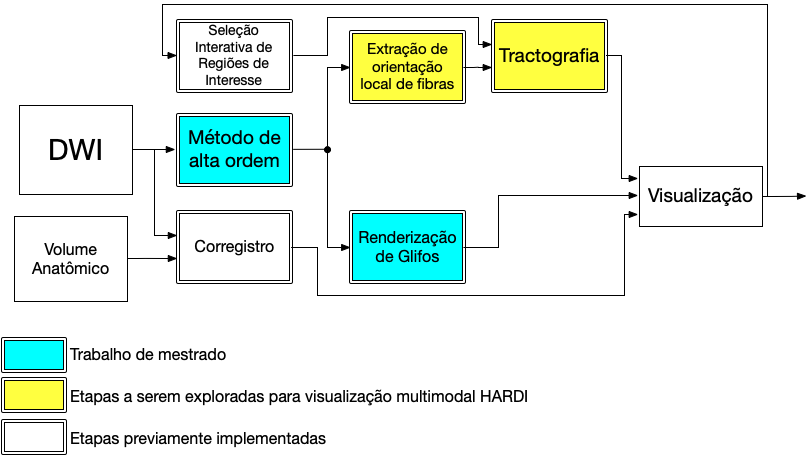
\includegraphics[width=.9\linewidth, angle=0]{figs/Introducao/fluxograma_VMTK_HARDI.png}
    \caption{Fluxograma do ambiente de visualização multimodal HARDI. Os capítulos \ref{chapter::metodos_hardi} e \ref{chap::renderizacao_de_perfis_de_difusao} trazem o detalhamento dos blocos destacados em azul.}
    \label{fig::flowchart_vmtk_hardi}
\end{figure}




%\todo[inline]{Principal motivação é aprimorar a interatividade no processo de reconstrução de uma fibra? Diante dos desafios ainda em aberto, espera-se que, através de uma visualização interativa dos dados de difusão HARDI devidamente pré-processados, um especialista junto com uma máquina construa de forma mais fiel possível, e não-invasiva, as fibras dos tratos (conhecidos e desconhecidos)?}

%\textcolor{red}{No que diz respeito ao método de síntese de orientações das fibras a partir dos volumes HARDI, integramos a sua formulação matemática diretamente no VMTK-Neuro. Os principais critérios para sua escolha se devem a sua adequabilidade em tractografia, sua aplicabilidade em DWIs de baixa resolução angular e simplicidade em relação a quais métodos???.}

%\todo[inline]{Dentre o estado-da-arte da tecnologia HARDI, qual aspecto te chamou atenção e te motivou a desenvolver este trabalho de Mestrado com o objetivo de "implementar e validar um algoritmo (melhor?) de tractografia baseada na técnica de imageamento HARDI"? Na forma como está colocada a sua proposta leva o leitor questionar se o trabalho é simplesmente um exercício do que já se tem.}

%\textcolor{red}{O conhecimento sobre tratos é ainda precário para reconstruí-los integral e automaticamente. É necessária a análise humana para assegurar a plausibilidade das conexões das amostras de múltiplas orientações que a técnica HARDI provê. Para que um especialista possa ter uma visão sucinta e precisa sobre as informações da difusividade local de uma amostra e ajudar uma máquina tomar decisão na ligação desta amostra com as amostras vizinhas para formar uma fibra, é desejável que ele explore de forma interativa tanto os perfis de difusão em cada amostra como as fibras reconstruídas com base nas conjeturas formuladas e reformuladas.}

\section{Ambiente de Implementação}
\label{ssec:ambiente}

Todas as implementações e experimentos do trabalho são realizados no aplicativo VMTK-Neuro (\textit{Visual Manipulation ToolKit for Neuroimages}) \cite{VMTKNeuro}, que é um ambiente de visualização exploratória multimodal multi-plataforma desenvolvida e mantida pelo grupo de pesquisa da Faculdade de Engenharia Elétrica e de Computação da UNICAMP ao qual faço parte. O \textit{software} renderiza em tempo real volumes de ressonância magnética (\textit{magnetic resonance imaging} - MRI) e possui ferramentas de exploração para volumes DWI a partir do DTI. 





%Na subseção \ref{ssec:vmtk-neuro} do capítulo Materiais e Métodos, ilustramos as ferramentas para DWI como um fluxograma e descrevemos as funcionalidades correlatas ao presente trabalho.

% conforme mostrado no fluxograma da figura \ref{fig::PipelineDTI_tracto}.%\textcolor{red}{escaneados com o protocolo Overplus \cite{Philips} e de rastreamento das fibras para volumes DTI sintetizados a partir de DWIs}\todo{não necessariamente Overplus. Overplus não sintetiza as sequencias de aquisições de DWI que há por aí.}.

%\begin{figure}[ht]
%   \centering
%       \addtolength{\leftskip} {-2cm} % increase (absolute) value if needed
%    \addtolength{\rightskip}{-2cm}
%
%    %\vspace*{3mm}
%    \centering
%    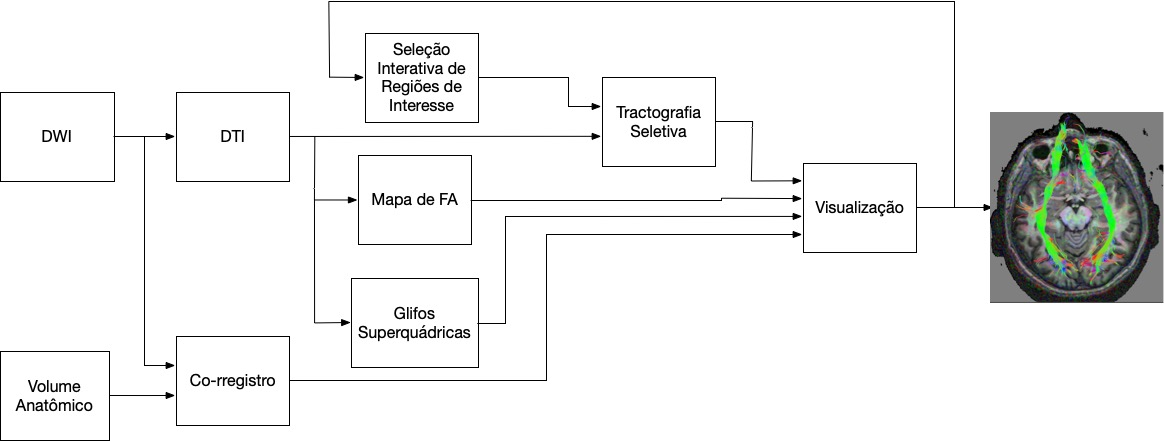
\includegraphics[width=1.0\linewidth, angle=0]{figs/Fluxogramas/PipelineDTI_tracto.jpg}
%    \caption{Fluxograma para tractografia implementado no VMTK-Neuro.}
%    \label{fig::PipelineDTI_tracto}
%\end{figure}

%Estas ferramentas consistem na visualização em tempo interativo de tensores de difusão mapeados em glifos superquádricos \cite{Kindlmann2004} renderizados sobre as suas respectivas amostras (figura \ref{fig::intro_ex_DTI_glifos}), tractografia (figura \ref{fig::intro_ex_DTI_tractografia}) e o corregistro de volumes de difusão com volumes anatômicos T1.

%Na tractografia baseada em DTI, o VMTK-Neuro possui ferramentas de interatividade que possibilitam que o usuário possa inferir sobre as regiões do volume que contém os tratos a serem analisados, bem como filtrar fibras de interesse e eliminar fibras espúrias. Adicionalmente, parâmetros relacionados a reconstrução, que podem diferir de acordo com a região de análise do usuário, também são configuráveis. O algoritmo de tractografia apresenta resultados visuais em tempo interativo para as formas de interação mencionadas.




\section{Objetivos}
\label{sec::objetivos}

As ferramentas de visualização O ambiente de visualização multimodal, que integra diferentes modalidades de neuroimagens, incluindo a ressonância de difusão modelada pelo DTI, de forma co-registrada, e, adicionalmente um algoritmo de tractografia interativo, baseado em \citeonline{Weinstein1999}.


Motivados pela pesquisa que evidenciam as vantagens da tractografia baseadas em métodos mais avançados em aquisições de alta resolução angular, temos a intenção de fazer a visualização multimodal com DWIs através de algum.

Para alcançar este objetivo, podemos esquematizar os passos em quatro sub-problemas:

\begin{enumerate}
    \item a implementação de um método de imageamento de alta ordem para difusão;
    \item a visualização multimodal dos dados que descrevem a difusão através do método em glifos;
    \item Cômputo da distribuição de fibras a partir dos dados obtidos através do método, que é feito de forma local, \textit{voxel} a \textit{voxel}; e
    \item implementação de um algoritmo de tractografia interativo a partir da distribuição de orientação de fibras.
\end{enumerate}


Glifos relacionados a funções obtidas através de métodos HARDI são amplamente utilizados como prova de conceito visual na pesquisa da área. Sua visualização interativa, onde estes objetos são renderizados sobre as suas respectivas regiões no volume melhora a qualidade da pesquisa na área \cite{peeters2009}. Adicionalmente, temos a conjectura que os glifos possam ser utilizados para detectar anormalidades nas neuroimagens, bem como servir de suporte visual para escolha de parâmetros iniciais em tractografia, conforme evidenciado em \citeonline{voltoline2021} para superquádricos do DTI.

Cumprindo estes objetivos, estaremos aptos a fazer pesquisas na área de tractografia, tanto no que diz respeito a contribuição em métodos e algoritmos, quanto em aplicações clínicas. Sobre a métodos de tractografia, \citeonline{SCHILLING2019194} menciona os desafios, oportunidades e limitações nesta área de tractografia, e menciona que a próxima evolução em tractografia há de vir a partir do uso de outras fontes de informação, no qual podemos ter futuras conjecturas para investigação em como podemos utilizar dados co-registrados em adição ao DWI para dar passos adicionais nesta área.




\section{Contribuições}
\label{sec:contribuicoes}

A contribuição esperada para o presente trabalho dentro do escopo do ambiente exploratório para DWI através de métodos avançados de imageamento é a implementação de um método avançado para difusão, no qual escolhemos a amostragem generalizada no espaço-Q (GQI - \textit{Generalized Q-Space Imaging}) \cite{yeh2010} e a validação de um algoritmo de renderização interativo de glifos que sintetize o perfil de difusão gerado pelo método integrado ao ambiente de visualização exploratória multimodal interativo como um protótipo, como ilustrado no fluxograma da Fig. \ref{fig::flowchart_vmtk_hardi}.




%\textcolor{red}{A expectativa é aplicar os resultados na implementação do fluxograma mostrado na Figura ??? no VMTK-Neuro ...}



%\todo[inline]{Sugiro que mostre em algum ponto uma visão geral do fluxo de controle da sua proposta de construção de tractografia a partir de DWIs de alta resolução angular.}

\section{Desafios}
\label{sec::desafios}

Para implementação do sistema, muito da infraestrutura necessária para alcançar os objetivos estabelecidos estão implementadas no VMTK-Neuro para visualização de volumes DWI por DTI. Portanto, muitos dos desafios enfrentados dizem respeito a questões de implementação do método HARDI e seu esquema de visualização em glifos.

A própria implementação matemática de um método HARDI para sintetizar o perfil de difusão é uma tarefa desafiadora. Os métodos demandam uma quantidade de memória razoavelmente maior que o DTI, que pode ser codificado na memória com apenas 6 elementos (matriz 3x3 simétrica). Métodos HARDI não estabelecem um critério mínimo, entretanto é usual que centenas de elementos sejam utilizados para descreverem o perfil de difusão de forma razoável.

A implementação de um esquema de renderização de perfis de difusão em tempo interativo é algo desafiador pela grande quantidade de dados necessários para sintetizar um glifo. Além disso, o algoritmo de renderização é integrado ao pipeline da renderização multimodal volumétrica baseada em \textit{ray-casting} de volumes de ressonância magnética, o que diminui a margem de tempo de execução do esquema para manter a interatividade.

%O último desafio diz respeito à implementação de um algoritmo em tempo interativo de tractografia, que precisa ter seu cômputo rápido o suficiente para seguir as interações feitas pelo usuário.


%\todo[inline]{Não acha que aqui você tem que focar nos desafios relacionados à interatividade, uma vez que o item 4 listado na seção anterior já se encontra implementado no VMTK. Só precisa de algumas adequações. Quais são os desafios para tornar um algoritmo de reconstrução de fibras a partir de HARDI (DWI de alta resolução angular) interativo? Quais restrições devem ser observadas?}

%\sout{No que diz respeito à escolha do método HARDI utilizado, integramos a sua formulação matemática diretamente no VMTK-Neuro. Os principais critérios para sua escolha se devem a sua adequabilidade em tractografia, sua usabilidade em DWIs de baixa resolução angular e simplicidade.}

%\sout{Pela demanda de visualização interativa do VMTK-Neuro, objetivamos que a visualização dos perfis de difusão do método HARDI para os voxels visíveis na tela seja em tempo interativo. Assim, o usuário tem a informação em tempo real dos perfis de difusão nas regiões do volume a serem analisadas.}

%\sout{Assim como a visualização dos perfis de difusão, também objetivamos a visualização interativa da tractografia. As vantagens desta abordagem consistem em dar ao usuário o poder de, através da visualização, escolher regiões de análise e setar os melhores parâmetros de acordo com o seu trato de interesse, indivíduo analisado e aquisição DWI.}

%\section{Contribuições}
%\label{sec::contribuicoes}
%
%
%Este trabalho apresenta duas contribuições:
%
%\begin{itemize}
%	\item proposição de um algoritmo para visualização em tempo %interativo de perfis de difusão para métodos HARDI e
%	\item proposição e validação de um algoritmo de tractografia %em tempo interativo baseado em informações direcionais de %fibras.
%\end{itemize}


%O trato corticoespinhal (CST) (Figura \ref{fig::CST_anatomia}) será o ponto de partida de análise e um ponto central para validação do algoritmo para o escopo deste trabalho de mestrado.

\section{Organização}
\label{sec:intro_organizacao}

O trabalho está organizado em quatro capítulos. No Capítulo \ref{chapter::metodos_hardi}, descreveremos brevemente sobre as aquisições DWI, a motivação para utilização de métodos HARDI para modelar a difusão, detalharemos a implementação do método GQI, tanto no que diz respeito a sua formulação matemática, como a sua implementação computacional; no capítulo \ref{chap::renderizacao_de_perfis_de_difusao} detalharemos o algoritmo de renderização para glifos que sintetizam ODFs integrado ao VMTK-Neuro atrelado a renderização de um volume \textit{ray-casted}, com sua respectiva validação visual e performance computacional; no capítulo \ref{chap::conclusao}, concluímos o trabalho e mencionamos oportunidades de trabalhos futuros.

%\chapter{Materiais e Métodos}

%\section{Materiais}






%\subsection{VMTK-Neuro}
%\label{ssec:vmtk-neuro}

%O VMTK-Neuro é um \textit{software} que renderiza em tempo real volumes de ressonância magnética (\textit{magnetic resonance imaging} - MRI) e possui ferramentas de exploração para volumes DWI a partir do DTI, conforme mostrado no fluxograma da figura \ref{fig::PipelineDTI_tracto}. O software utiliza a linguagem de programação em C++ e o OpenGL como API gráfica.

%\begin{figure}[ht]
%   \centering
%       \addtolength{\leftskip} {-2cm} % increase (absolute) value if needed
%    \addtolength{\rightskip}{-2cm}
%
%    %\vspace*{3mm}
%    \centering
%    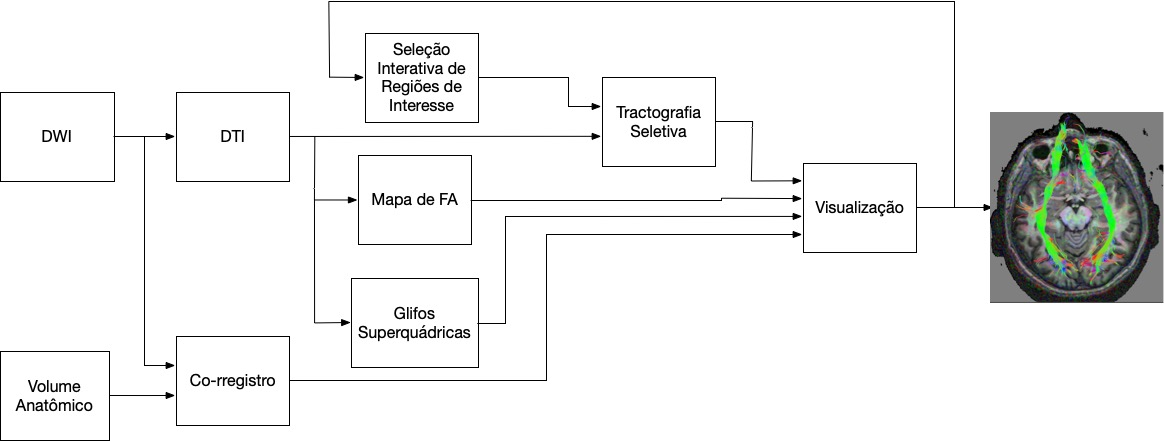
\includegraphics[width=1.0\linewidth, angle=0]{figs/Fluxogramas/PipelineDTI_tracto.jpg}
%    \caption{Fluxograma para tractografia e glifos implementado no VMTK-Neuro.}
%    \label{fig::PipelineDTI_tracto}
%\end{figure}

%Estas ferramentas consistem na visualização em tempo interativo de tensores de difusão mapeados em glifos superquádricos \cite{Kindlmann2004} renderizados sobre as suas respectivas amostras (figura \ref{fig::intro_ex_DTI_glifos}), tractografia (figura \ref{fig::intro_ex_DTI_tractografia}) e o corregistro \cite{ting2014} de volumes de difusão com volumes anatômicos T1 .



%Na tractografia baseada em DTI, o VMTK-Neuro possui ferramentas de interatividade que possibilitam que o usuário possa inferir sobre as regiões do volume que contém os tratos a serem analisados, bem como filtrar fibras de interesse e eliminar fibras espúrias. Adicionalmente, parâmetros relacionados a reconstrução, que podem diferir de acordo com a região de análise do usuário, também são configuráveis. O algoritmo de tractografia apresenta resultados visuais em tempo interativo para as formas de interação mencionadas.


%\subsection{Volumes}

%%%%%VOLUMES UTILIZADOS NOS EXPERIMENTOS


%Temos a intenção de fazer a investigação com dados reais de pacientes do Hospital das Clínicas da UNICAMP, cujo uso foi aprovado pelo comitê de ética CAAE 0893.0.146-000.09, 


%No decorrer do trabalho tínhamos a intenção de usar o volumes do bancos de dados do Hospital das Clínicas da UNICAMP, porém os resultados preliminares em termos de conjuntos de ODFs obtidos não se mostraram adequados, e descartamos o uso. Fizemos um estudo para diagnosticar a natureza do problema, que está detalhado na subseção \ref{ssec::problema_overplus} do apêndice, e concluímos que está relacionado ao conjunto de gradientes de ponderação de difusão utilizado no padrão \textit{Overplus}.


%\section{Métodos}
%\subsection{Interatividade}

%Pela demanda de visualização interativa do VMTK-Neuro, objetivamos que a visualização dos perfis de difusão de glifos ODF para as amostras visíveis na tela aconteça em tempo interativo. Sendo assim, documentaremos os \textit{benchmarks} de ambos sistemas para atestar o cumprimento deste objetivo.

%\subsection{Tractografia}

%A motivação principal desde trabalho nasceu da seguinte pergunta: "como podemos melhorar a tractografia baseada em DTI do VMTK-Neuro?". Neste contexto, iremos comparar a tractografia baseada em DTI implementada no VMTK-Neuro e a tractografia baseada em HARDI em tratos que há a documentação de falhas do DTI e que são resolvidos pela abordagem que utiliza métodos HARDI.





%\textcolor{red}{
\chapter{Imageamento de alta resolução angular para difusão}
\label{chapter::metodos_hardi}
%}

Neste capítulo iremos descrever uma introdução e motivação de métodos HARDI, o método escolhido para sua implementação no VMTK-Neuro, bem como os detalhes computacionais de sua implementação.

Na Seção \ref{sec::aquisicao_dwi}, faremos uma breve descrição da sequencia de aquisição de um DWI, no que diz respeito as grandezas envolvidas e parâmetros associados, mas sem entrar nos detalhes da física; na Seção \ref{sec::dti_limitacoes_hardi}, trazemos uma descrição breve do DTI, suas limitações e a motivação do uso de métodos de mais alta ordem e aquisições de mais alta resolução; na Seção \ref{sec::gqi}, descrevemos o principio do método da amostragem generalizada no espaço-Q, no qual mostramos a base teórica, sintetizamos a transformada que leva os sinais de difusão para amostras que sintetizam o comportamento de difusão subjacente através de uma multiplicação matricial, formulamos o domínio de amostragem da transformada e adicionalmente, visando otimizar o uso de memória, exploramos a simetria do comportamento de difusão para associar diminuir a quantidade de amostras associadas ao domínio armazenadas na memória.

Neste capítulo, trazemos a formulação do conceito de função de distribuição de orientação (ODF - \textit{orientation distribution function}) é a base para as discussões do capítulo \ref{chap::renderizacao_de_perfis_de_difusao}, em que detalhamos um esquema de renderização para visualização dos perfis de difusão obtidos através do imageamento.

\section{Aquisição DWI}
\label{sec::aquisicao_dwi}
A sequência de pulsos PGSE (\textit{Pulsed Gradient Spin Echo}), é comumente utilizada para inserir a componente de difusão molecular no sinal de MRI, e é normalmente combinada à sequência  EPI (\textit{Echo-Planar Imaging}) de aquisição de MRI. Uma introdução ao assunto pode ser encontrada em \citeonline{DTI_Handbook}, os fundamentos de imageamento por MRI e sequencia de pulsos do EPI pode ser encontrada em \citeonline{liang2000}, e a física da difusão e seu imageamento via PGSE integrado ao EPI pode ser encontrado em \citeonline{tuch2002}. Nesta seção, faremos uma introdução das grandezas envolvidas na aquisição, faremos uma introdução ao espaço-Q, e mostramos como é a formulação das amostras de difusão neste espaço a partir de parâmetros acessíveis em aquisições DWI. Usaremos esta formulação para derivação do GQI na seção \ref{sec::gqi}.

Fig. \ref{fig::pgse_ilustrado} ilustra o processo de medição de difusão no qual dois gradientes de ponderação de difusão são aplicados em uma direção $\mathbf{\hat{q}}$ e amplitude $G$. Antes da aplicação do gradiente (período $t_1$), os núcleos de hidrogênios tem seus respectivos spins em fase, oscilando na mesma frequência, chamada de frequência de Larmour $f = \gamma \cdot B_0$, onde $\gamma$ é a razão giromagnética do núcleo de hidrogênio e $B_0$ é a magnitude do campo magnético estático principal que excita os spins na sequência EPI. O sinal gerado é forte com frequência $f$.

\begin{figure}[ht]

%\subfigcapskip = -5pt
    \centering
    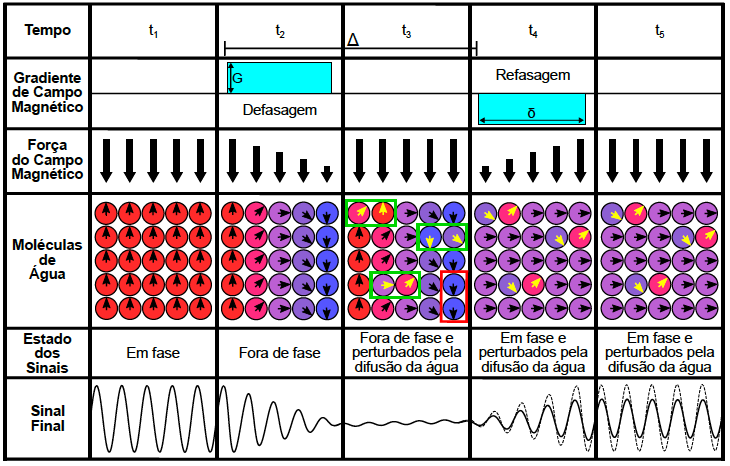
\includegraphics[width=.8\linewidth, angle=0]{figs/HARDI/pgse.png}
    \caption{Ilustração da medição de difusão das moléculas de água realizada na aquisições DWI nos \textit{scanners} de MRI \\
    Fonte: \cite{voltoline2016}
    }
    \label{fig::pgse_ilustrado}
   \hspace{1pt}
\end{figure}

Em $t_2$, o gradiente de intensidade $G$ e duração $\delta$ é aplicado, o gradiente é um campo magnético que varia linearmente ao longo da direção $\mathbf{\hat{q}}$ e  modifica a frequência de oscilação dos spins do núcleo hidrogênio. Quando o gradiente cessa $(t_3)$, os núcleos voltam a ter a mesma frequência de oscilação do período $t_1$, mas com fases diferentes, levando a intensidade do sinal ser enfraquecida.

Depois de um intervalo $\Delta$ a partir do início da aplicação do primeiro gradiente, o processo de equalizar as fases é inicializado utilizando um novo gradiente com mesma intensidade e duração, mas com sentido oposto em relação ao primeiro. Os núcleos pertencentes as moléculas que se difundiram na direção $\mathbf{\hat{q}}$ durante o intervalo $\Delta$, destacados em verde na janela de tempo $t_3$, terão suas fases corrigidas de forma a não ter a fase inicial novamente, pois estavam em lugares diferentes no espaço, consequentemente estando sob campos magnéticos diferentes nos instantes de defasagem e equalização de fase.

O sinal resultante em $t_5$ é atenuado em relação ao sinal ao intervalo $t_1$ (que está tracejado no instante $t_5$), devido a diferença de fase dos spins. Consequentemente, diz-se que o sinal está ponderado em difusão.


A atenuação da ponderação por difusão pode ser configurada através da manipulação dos parâmetros  $G$, $\delta$ e $\Delta$. Para sequência PGSE, é comum estas grandezas serem sintetizadas em um fator de ponderação de difusão chamado de valor $b$. Sua formulação em função dos parâmetros de difusão é dada por \cite{DTI_Handbook}:

\begin{equation}
\label{eq::bvalue}
    b = \gamma^2G^2\delta^2(\Delta - \frac{\delta}{3})
\end{equation}

Nesta dissertação, nós usaremos o termo "volume" ~para referenciar uma imagem 3D composta por imagens 2D e o termo "fatia" ~para referenciar estas imagens 2D. Será usado também o termo "aquisição DWI" quando quisermos referenciar, de uma vez, o conjunto de volumes escaneados numa sessão de aquisição e o termo "resolução angular" com a quantidade de volumes ponderados por difusão em uma aquisição DWI. Nós adotamos o termo "\textit{b0}"  para referenciar volumes não-ponderados em difusão em uma aquisição DWI.

As aquisições de difusão são modeladas como amostras no espaço-Q, que consiste em um espaço tridimensional no qual os sinais de difusão no \textit{voxel} $\mathbf{r}$, $W(\mathbf{r}, \mathbf{q})$ é amostrado no ponto representado por $\mathbf{q} = (\gamma G \delta)/2\pi \cdot \mathbf{\hat{q}}$\footnote{\citeonline{tuch2002} representa esta relação por $\mathbf{q} = (\gamma G \delta)\cdot \mathbf{\hat{q}}$} \cite{yeh2010}. A partir destas amostras, métodos de imageamento, como o DTI, são utilizados para inferir sobre o perfil de difusão e a distribuição direcional de fibras \textit{voxel} a \textit{voxel}. A amostragem no espaço-Q em função dos valores $b$ de uma aquisição pode ser mostrada substituindo os parâmetros de aquisição que geram $\mathbf{q}$ pela formulação de $b$ na Eq. \ref{eq::bvalue}, que está formulado na Eq. \ref{eq::qspace_bvalue}, onde $\tau = \Delta - \delta/3$.

\begin{equation}
\label{eq::qspace_bvalue}
\mathbf{q} = \frac{1}{2\pi}\sqrt{\frac{b}{\tau}} \mathbf{\hat{q}}
\end{equation}

A respeito dos valores $b$ utilizados em uma aquisição DWI, e como utilizá-los no espaço-Q, há normalmente três estratégias de amostragens para a aquisição:

\begin{enumerate}
    \item amostragem cartesiana, onde as amostras são igualmente espaçadas no espaço-Q em um espaço cartesiano tridimensional e que é usualmente associado ao imageamento de espectro por difusão (DSI) \cite{wedeen2005};
    \item amostragem \textit{single-shell}, que consiste na amostragem feita para um valor b constante, que está contido numa esfera no espaço-Q;
    \item amostragem \textit{multi-shell}, que consiste na amostragem que consiste em diferentes conjuntos de pontos contidos em mais de uma esfera, que se referem a uma quantidade no espaço-Q.
\end{enumerate}

%Dado um conjunto de amostras de sinais de difusão no espaço-Q, há diversas técnicas para descrever o processo de difusão \textit{voxel} a \textit{voxel} sumarizá-los em potenciais caminhos de fibras, sendo o DTI \cite{Basser1994} a mais utilizada.


\section{DTI, limitações e HARDI}
\label{sec::dti_limitacoes_hardi}
%\todo[inline]{Sugiro que façs aqui uma espécie de survey dos métodos ... Fica a seu critério a classificação ... pode ser por forma de amostragem como em \url{https://www.researchgate.net/publication/319558026_High_Angular_Resolution_Diffusion_Imaging_HARDI/link/59e88db8a6fdccfe7f8e8a4f/download} ... Sugiro que poderia fazer um merge com capítulo 3.}

%Na aquisição do DWI, é escaneado um conjunto de volumes em que cada um possui a ponderação de único gradiente de difusão associado a um valor-b\footnote{O valor-b é uma métrica de sensitividade para difusão e é função de parâmetros da aquisição do DWI, como função da intensidade, duração e o intervalo de tempo dos gradientes de ponderação de difusão. Quanto maior o seu valor, maior o decaimento do sinal relativo à difusão.}, e, adicionalmente, um ou mais volumes sem ponderação de gradiente, denominado volume b0. A quantidade de volumes ponderados para diferentes direções de gradiente é denominada de resolução angular. Técnicas para sumarizar os sinais coletados em informações de potenciais caminhos de fibras nervosas são objeto de pesquisa desde o início dos anos 90 \cite{descoteaux2015}.

O método DTI \cite{Basser1994} consiste em um mapeamento das amostras de difusão em um ponto contido em uma aquisição DWI em um modelo gaussiano, que é sintetizada por tensor de ordem 2, representado por uma matriz 3x3 simétrica (Eq. \ref{eq::tensor}). Para seu cômputo, o DTI necessita de no mínimo seis volumes ponderados por difusão em adição a um $b0$, nos quais geram um sistema para cômputo dos seis coeficientes do tensor. Na prática, os volumes DWI escaneados para serem usados com este método, que é predominante no uso clínico, varia entre 6 e 32 \cite{descoteaux2015}.


\begin{equation}
\label{eq::tensor}
\mathbf{D} = 
\begin{bmatrix}
D_{xx} & D_{xy} & D_{xz} \\ 
D_{xy} & D_{yy} & D_{yz} \\ 
D_{xz} & D_{yz} & D_{zz}  
\end{bmatrix}
\end{equation}

Usualmente, a informação referente ao processo de difusão é comumente extraída dos seus três autovetores e autovalores. Entretanto, o método apresenta limitações.

A limitação do DTI acerca da possibilidade de inferir sobre fibras subjacentes é vinculada a modelagem da difusão ao modelo Gaussiano. O modelo descreve bem regiões de fibras em que o comportamento de difusão ocorre predominantemente em uma direção. Em pontos que contém múltiplas fibras e que estão dispostas nas mais variadas configurações (por exemplo: cruzamento, bifurcação, mistura, "beijo") o modelo gaussiano não sintetiza de forma correta o comportamento da difusão, impedindo o cômputo das direções plausíveis para reconstrução de uma fibra de interesse \cite{fillard2011, daducci2014}. Há um estimativa que entre 66\% a 90\% da substância branca do cérebro contém múltiplas configurações de cruzamento de fibra \cite{descoteaux2015} e a limitação do DTI é um obstáculo para modelar as direções de fibras subjacentes de forma adequada.


Devido as limitações do DTI para inferir sobre a matéria branca do cérebro na resolução de cruzamento de fibras, houve uma agenda de pesquisa que começa no início da década de 2000 de proposição de métodos de imageamento para transformação do sinal de difusão em um modelo, e consequentemente houve uma demanda por uma maior resolução angular nas aquisições DWI, denominadas de imageamento difusão de alta resolução angular para difusão (HARDI - \textit{high angular resolution diffusion imaging}). Tipicamente aquisições HARDI \textit{single-shell} contém 45 volumes ponderados por e $1000 \leq b \leq 4500$ $s/mm^2$.


Houve mais de cem artigos que propuseram métodos de imageamento para transformação do sinal de difusão para o seu perfil de difusão/distribuição de fibras entre 2000-2010 \cite{descoteaux2015}. Os métodos consistem em técnicas para síntese do sinal de difusão em funções de distribuição de orientação (ODF) que dão a possibilidade de inferir sobre a distribuição de fibras subjacente.

Uma ODF consiste em uma associação entre direções, usualmente representadas por um vetor unitário $\mathbf{\hat{u}}$ (ou par $(\theta, \phi)$ em coordenadas esféricas), em um valor escalar $\psi(\mathbf{\hat{u}})$. Em geral, os métodos podem ser categorizados de duas formas de acordo com a natureza da técnica de transformada do sinal de difusão para a ODF que gera a configuração de fibras subjacentes: técnicas livres de modelo e técnicas de modelos misturados. 

As técnicas livres de modelo buscam formular uma representação para formulação da função de difusão explorando a relação de Fourier \cite{tuch2002} do sinal de difusão $W(\mathbf{r}, \mathbf{q})$ para obtenção de características da difusão em seu perfil angular $\psi(\mathbf{\hat{u}})$. Entre os métodos foram propostos, o DSI \cite{wedeen2005}, proposto originalmente em 2000 e presente na tese de doutorado de \citeonline{tuch2002}, juntamente com o QBI, proposto em \citeonline{TuchQBall2004} em sua forma de artigo, e o GQI \cite{yeh2010} exemplificam esta categoria de métodos.

Técnicas de modelos misturados assumem que o sinal de difusão medido para um \textit{voxel} é a soma dos sinais gerados por cada população de fibra presente nele \cite{tournier2011}. Como exemplos, há a abordagem multi-tensor, também presente na tese de doutorado de \citeonline{tuch2002}, e a abordagem por deconvolução esférica, proposta originalmente por \citeonline{Tournier2004DirectEO}.

A abordagem multi-tensor modela a difusão como uma soma ponderada de modelos Gaussianos, com diferentes tensores associados a cada um. Enquanto na abordagem por deconvolução esférica, há a conjectura que o sinal de difusão é gerado a partir da resposta da fibra ao gradiente de ponderação de difusão e este fenômeno é representado por uma convolução da função de distribuição de orientação de fibras (fODF) por uma função resposta para uma fibra única. Assim, a fODF é reconstruída a partir de uma técnica de deconvolução.


%!!Porque geram ODFs?

%Estes métodos geram uma ODF a partir do sinal de difusão. Geralmente ODFs não possui a restrição quanto a regressão uma função tridimensional que o DTI possui e portanto conseguem ser mais descritivos do processo de difusão e gerar boas aproximações das fibras subjacentes, especialmente em cruzamentos \cite{daducci2014}.

% e evidentemente precisamos fazer uma seleção dos quais deles são mais relevantes para o nosso trabalho.

Há diferentes aplicativos livres que utilizam métodos HARDI para processamento de DWI, que estão ligados a grupos de pesquisa na área, alguns destes aplicativos utilizam o GQI (DSI-Studio\footnote{Disponível em: http://dsi-studio.labsolver.org}), QBI (FSL\footnote{Disponível em: https://fsl.fmrib.ox.ac.uk/fsl/fslwiki/FSL}, FiberNavigator\footnote{Disponível em: https://scilus.github.io/fibernavigator/}), ambos métodos livres de modelo, e o \textit{constrained spherical deconvolution} \cite{tournier2007} (MRTrix\footnote{Disponível em: https://www.mrtrix.org/}), que é uma abordagem de deconvolução esférica.


Escolhemos o GQI para ser implementado no VMTK-Neuro para que possamos fazer pesquisas em torno dele. Sua escolha se deu por possuir as seguintes características \cite{yeh2010}:

\begin{enumerate}
    \item Ser aplicável em categorias de aquisição com múltiplos valores $b$;
    \item boa aplicabilidade em volumes de mais baixa resolução angular;
    \item ter parâmetros de regularização e filtragem integrados ao método, o que é necessário para o cômputo da distribuição de fibras subjacentes.
\end{enumerate}

Um ponto importante no processo de decisão na implementação é referente a adequabilidade em tractografia. Segundo \citeonline{daducci2014}, no seu trabalho sobre comparações de diferentes métodos de imageamento em tractografia, não há métodos que se sobressaem em relação a outros nas mais diferentes condições experimentais.

%A grande desvantagem do GQI implementado na forma proposta por \citeonline{yeh2010} ocorre no uso de memória. A codificação de ODFs é feita por amostras e requer uma grande quantidade de memória, usualmente nas centenas de números por \textit{voxel}. Métodos que armazenam os dados como coeficientes de função base, como o QBI formulado por \citeonline{descoteaux2007_QBI} e o CSD \cite{tournier2007} tendem a utilizar menos memória.

\section{Amostragem Generalizada no Espaço Q}
\label{sec::gqi}
\subsection{Formulação}

O GQI é um método de modelo livre, derivado da relação de Fourier entre o sinal de difusão e o deslocamento dos spins devido à difusão. O método é baseado na relação da função de distribuição de \textit{spins} (\textit{spin distribution function} - SDF) $\psi_Q(\mathbf{r}, \mathbf{\hat{u}})$ em função de $W(\mathbf{r}, \mathbf{q})$.

Para isso, o método explora a relação de Fourier em três dimensões entre o sinal de difusão $W(\mathbf{r}, \mathbf{q})$ e a função de densidade de spins $Q(\mathbf{r}, \mathbf{R})$:

\begin{equation}
\label{eq::spin_diffsignal_1}
    Q(\mathbf{r}, \mathbf{R}) =
    \int \! W(\mathbf{r}, \mathbf{q})e^{-i2\pi \mathbf{q}\cdot \mathbf{R} } \,\mathrm{d}\mathbf{q}
\end{equation}

Como $Q(\mathbf{r}, \mathbf{R})$ é real e $W(\mathbf{r}, \mathbf{q})$ é simétrica, podemos considerar a parte real da transformada, fazendo a expressão se tornar:

\begin{equation}
\label{eq::spin_diffsignal_2}
    Q(\mathbf{r}, \mathbf{R}) =
     \int \! W(\mathbf{r}, \mathbf{q})\text{cos}(2\pi \mathbf{q}\cdot \mathbf{R}) \,\mathrm{d}\mathbf{q}
\end{equation}

Por outro lado, podemos estimar a quantidade de spins que se submetem a difusão em um direção $\mathbf{\hat{u}}$ através da integração da função $Q(\mathbf{r}, \mathbf{R})$ nesta direção, o que resulta na SDF $\psi_Q(\mathbf{r}, \mathbf{\hat{u}})$:
\begin{equation}
\label{eq::sdf_spin}
    \psi_Q(\mathbf{r}, \mathbf{\hat{u}}) =
   \int_{0}^{L_{\Delta}} Q(\mathbf{r}, L\mathbf{\hat{u}})\!  \,\mathrm{d}L
\end{equation}
onde $L_\Delta$ é o comprimento de difusão na amostragem.

Combinando as Eq. \ref{eq::spin_diffsignal_2} e \ref{eq::sdf_spin}, obtemos a relação entre os sinais de difusão $W(\mathbf{r}, \mathbf{q})$ e a SDF $\psi_Q(\mathbf{r}, \mathbf{\hat{u}})$:
\begin{equation}
\label{eq::sdf_continuous_1}
    \psi_Q(\mathbf{r}, \mathbf{\hat{u}}) =
    \int_{0}^{L_{\Delta}}\int \! W(\mathbf{r}, \mathbf{q}) \text{cos}(2\pi L_{\Delta} \mathbf{q} \cdot \mathbf{\hat{u}}) \,\mathrm{d}\mathbf{q} \mathrm{d}L
\end{equation}
integrando em $L$, finalmente obtemos a expressão para obtenção da SDF em função do sinal de difusão: 
\begin{equation}
\label{eq::sdf_continuous_2}
    \psi_Q(\mathbf{r}, \mathbf{\hat{u}}) =
    L_{\Delta} \int \! W(\mathbf{r}, \mathbf{q}) \text{sinc}(2\pi L_{\Delta} \mathbf{q} \cdot \mathbf{\hat{u}}) \,\mathrm{d}\mathbf{q}
\end{equation}
onde $L_{\Delta}$ é o comprimento da amostragem de difusão, e $\text{sinc}(x) = \text{sin}(x)/x$ para todo $x$ real, exceto $0$, e $\text{sinc}(0) = 1$.

O cômputo da SDF discreta entre amostras oferecidas em uma aquisição DWI, rende uma SDF medida $\psi_m(\mathbf{r}, \mathbf{\hat{u}})$ de acordo com a Eq. \ref{eq::sdf_discrete_1}:

\begin{equation}
\label{eq::sdf_discrete_1}
    \psi_m(\mathbf{r}, \mathbf{\hat{u}}) =
     A_qL_{\Delta}\sum_{\mathbf{q} \in \mathbf{Q}} W(\mathbf{r}, \mathbf{q})\text{sinc}(2\pi L_{\Delta} \mathbf{q}\cdot\mathbf{\hat{u}})
\end{equation}

onde $A_q$ é uma termo de área constante de quadratura e $\mathbf{Q}$ corresponde as amostras no espaço-Q, dado por $\mathbf{Q}= [
\mathbf{q}_1,
\mathbf{q}_2,
\mathbf{q}_3, ...,
\mathbf{q}_T
]$. Observe que o comprimento de amostragem de difusão ajusta a contribuição de cada $W(\mathbf{r}, \mathbf{q})$ no cômputo de $\psi_m(\mathbf{r}, \mathbf{\hat{u}})$ e funciona como um parâmetro de regularização. Se $L_{\Delta}$ tende a infinito, a função de distribuição irá se comportar como um impulso na origem, gerando um $\psi_m(\mathbf{r}, \mathbf{\hat{u}})$ fortemente ponderado pelas direções de $\mathbf{q}$ ortogonais a $\mathbf{\hat{u}}$. Um $L_{\Delta}$ pequeno implica em uma maior ponderação para coeficientes que não são ortogonais a $\mathbf{\hat{u}}$, o que atua como uma filtragem, e o caso extremo de $L_{\Delta} = 0$ implica que todas os pesos aplicados para cômputo de ODFs para todo $\mathbf{\hat{u}}$ se tornem iguais.

Considerando que a difusão tem distribuição gaussiana, o comprimento de difusão é $(6D\tau)^{1/2}$, onde $D$ é o coeficiente de difusão da água na temperatura do corpo, dado por $3.0*10^{-3} mm^2/s$ \cite{yeh2019_DSI}, e $\tau = \Delta - \delta/3$. Podemos ponderar $L_{\Delta}$ por um fator $\sigma$ tal que $L_{\Delta} = \sigma(6D\tau)^{1/2}$. Para $\sigma$ = 1.3, $80\%$ da difusão é considerada no cômputo da SDF.

Obtemos a Eq. \ref{eq::sdf_discrete_2} substituindo $\mathbf{q}$ para parâmetros em função do valor $b$, mostrado na Eq. \ref{eq::qspace_bvalue}, e substituindo $L_{\Delta}$ por $\sigma(6D\tau)^{1/2}$ na Eq. \ref{eq::sdf_discrete_1}.



%Uma SDF é formada pela soma de várias SDF bases oferecidos por um esquema de amostragem. A relação entre o sinal de difusão é dada pela expressão:

\begin{equation}
\label{eq::sdf_discrete_2}
    \psi_m(\mathbf{r}, \mathbf{\hat{u}}) =
    A_qL_{\Delta}\sum_{\mathbf{q} \in \mathbf{Q}}W(\mathbf{r}, \mathbf{q})\text{sinc}(\sigma \sqrt{6D\cdot b(\mathbf{q})}\,\,  \mathbf{\hat{q}}\cdot\mathbf{\hat{u}})
\end{equation}

onde $W(\mathbf{r}, \mathbf{q})$ é o sinal de difusão no \textit{voxel} de coordenadas $\mathbf{r}$ e $\mathbf{\hat{q}} = \mathbf{q}/|\mathbf{q}|$. Na prática, as informações de ponderação de difusão em cada volume na aquisição DWI estão associados a um valor $b(\mathbf{q})$ e $\mathbf{\hat{q}}$. Vale a pena ressaltar que aquisições cujos sinais DWI são amostrados na metade de uma esfera para gradientes na direção $\mathbf{\hat{q}}$ tem o seu simétrico associado a ser adicionado em $\mathbf{Q}$, no qual tem o valor de sinal de difusão $W(\mathbf{r}, -\mathbf{q}) = W(\mathbf{r}, \mathbf{q})$.

O cômputo de ODFs é feito em $S$ amostras, nas quais são computadas através de um domínio de direções de interesse, dadas por $\mathbf{U} = [
\mathbf{\hat{u}}_1, 
\mathbf{\hat{u}}_2, 
\mathbf{\hat{u}}_3, ..., 
\mathbf{\hat{u}}_S 
]$,  em que queremos reconstruir um vetor ODF, dado por $\boldsymbol{\psi}(\mathbf{r}) = [
\psi(\mathbf{r}, \mathbf{\hat{u}}_1), 
\psi(\mathbf{r}, \mathbf{\hat{u}}_2), 
\psi(\mathbf{r}, \mathbf{\hat{u}}_3), \dots, 
\psi(\mathbf{r}, \mathbf{\hat{u}}_S)
]^T$, para cada \textit{voxel} de um volume DWI que tem um conjunto de sinais de difusão $\mathbf{W}(\mathbf{r}) = [
W(\mathbf{r},\mathbf{q}_1),
W(\mathbf{r},\mathbf{q}_2),
W(\mathbf{r},\mathbf{q}_3), \dots ,
W(\mathbf{r},\mathbf{q}_T)
]^T$. Detalharemos o processo de escolha de $\mathbf{U}$ na Subseção \ref{ssec::dominio_esferico}.

Assim, podemos computar as SDFs através de amostras pela multiplicação matricial da Eq. \ref{eq::gqi_vec}:

\begin{equation}
\label{eq::gqi_vec}
    \boldsymbol{\psi}_m(\mathbf{r}) = \mathbf{S}*\mathbf{W}(\mathbf{r})
\end{equation}

onde $\mathbf{S}$ é a matriz de transformação do sinal DWI para amostras de SDF no qual $s_{i,j}$ é dado por:

\begin{equation}
\label{eq::s_ij}
s_{i,j} = A_qL_{\Delta}\text{sinc}(\sigma \sqrt{6D.b(\mathbf{q}_j)} )\mathbf{\hat{q}}_j.\mathbf{\hat{u}_i})
\end{equation}

Com o objetivo de enfatizar as direções dominantes de difusão, optamos por normalizar cada SDF $\boldsymbol{\psi}_m(\mathbf{r})$ pela normalização min-max, obtendo assim a ODF $\boldsymbol{\psi}(\mathbf{r})$, conforme mostrado na Eq. \ref{eq::SDF2dODF}. A visualização do efeito da normalização está ilustrada na Fig. \ref{fig::normalizacao_min_max}. Observe que a normalização cancela o fator de escala $A_qL_{\Delta}$ da Eq. \ref{eq::s_ij}.

\begin{equation}
\label{eq::SDF2dODF}
    \boldsymbol{\psi}(\mathbf{r}) = \frac{\boldsymbol{\psi}_m(\mathbf{r}) - \text{min}(\boldsymbol{\psi}_m(\mathbf{r}))}{\text{max}(\boldsymbol{\psi}_m(\mathbf{r})) - \text{min}(\boldsymbol{\psi}_m(\mathbf{r}))}
\end{equation}

\begin{figure}[ht]
\centering
\captionsetup[subfloat]{farskip=0pt,nearskip=0pt}
\centering
    \subfloat[ODF não normalizada] {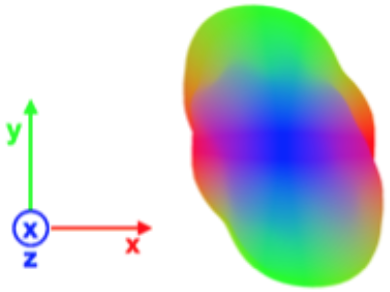
\includegraphics[width=.30\linewidth, angle=0]{figs/HARDI/ODF_normalizacao/ODF-pura.png}
    \label{fig::odf_pura}
    }
    \hspace{1em}
    \subfloat[ODF min-max normalizada] {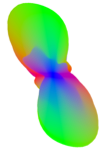
\includegraphics[width=.17\linewidth, angle=0]{figs/HARDI/ODF_normalizacao/ODF_minmax.png}
    \label{fig::odf_minmax}
    }
     \caption{Glifo ODF da mesma ODF com e sem a normalização min-max. A disposição de cores glifo enfatiza a orientação da ODF, no qual a direção dos eixos x, y, z estão mapeadas nas cores vermelha, verde e azul. Note que em \ref{fig::odf_minmax}, a estrutura orientacional da ODF é enfatizada com uma forte componente na direção do eixo y. O Capítulo \ref{chap::renderizacao_de_perfis_de_difusao} traz a formulação com detalhes do glifo.}
    \label{fig::normalizacao_min_max}
\end{figure}

\subsection{Domínio esférico}
\label{ssec::dominio_esferico}


Escolhemos os conjunto $\mathbf{U}$ baseado nas malhas esféricas obtidas através de subdivisões do icosaedro. Esta categoria de malha é amplamente utilizada pela comunidade HARDI. Além de \citeonline{yeh2010}, \citeonline{TuchQBall2004} a utiliza em seus respectivo experimento para ilustrar as suas respectivas ODF. Adicionalmente, \citeonline{descoteaux2007} usa esta categoria de malha para computar a distribuição de fibras adjacentes do QBI em seu respectivo algoritmo de tractografia. Algumas esferas aproximadas por tesselações do icosaedro estão ilustradas na Fig. \ref{fig::icosphere}. O conjunto $\textbf{U}$ é obtido em função vetores normais dos vértices da malha.

Neste trabalho, nos restringimos a categoria de malhas feitas através das subdivisões de ordem $2^k$ do icosaedro. Esta categoria de malha apresenta duas características desejáveis: a primeira se refere a presença de pares simétricos em relação aos eixos coordenados i. e., se o ponto $P$ está na malha, $-P$ também está; a segunda se refere a possibilidade de tirar proveito da percepção visual na renderização de glifos ODF, o que possibilita aumentar e diminuir a resolução dos glifos ODF de acordo com um modelo que relaciona sua ocupância na tela e resolução, conforme será detalhado no capítulo \ref{chap::renderizacao_de_perfis_de_difusao}.

\begin{figure}[ht]
\centering
\captionsetup[subfloat]{farskip=0pt,nearskip=0pt}
\centering
    \subfloat[Tesselação de $2^a$ ordem] {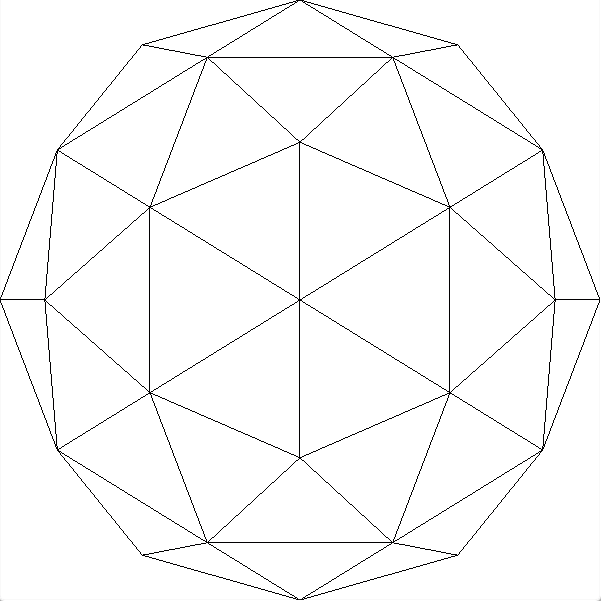
\includegraphics[width=.25\linewidth, angle=0]{figs/HARDI/Icosphere/icosphere_1.png}
    \label{fig::icosphere_1}
    }
    \hspace{1em}
    \subfloat[Tesselação de $4^a$ ordem] {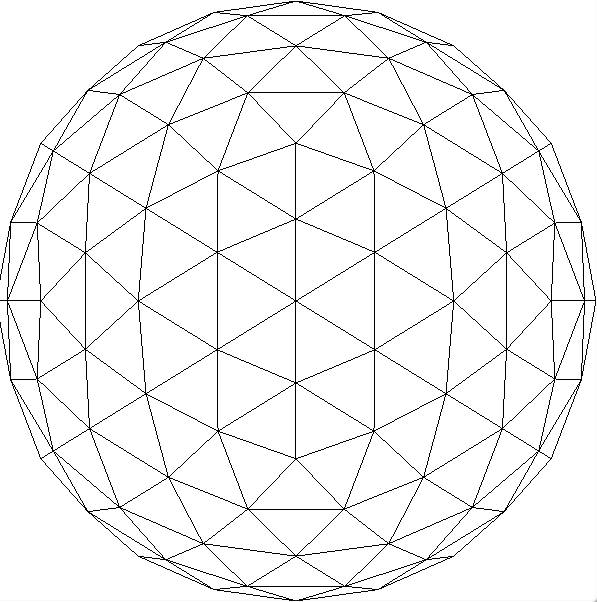
\includegraphics[width=.25\linewidth, angle=0]{figs/HARDI/Icosphere/icosphere_2.png}
    \label{fig::icosphere_2}
    }
    \\
    \subfloat[Tesselação de $8^a$ ordem] {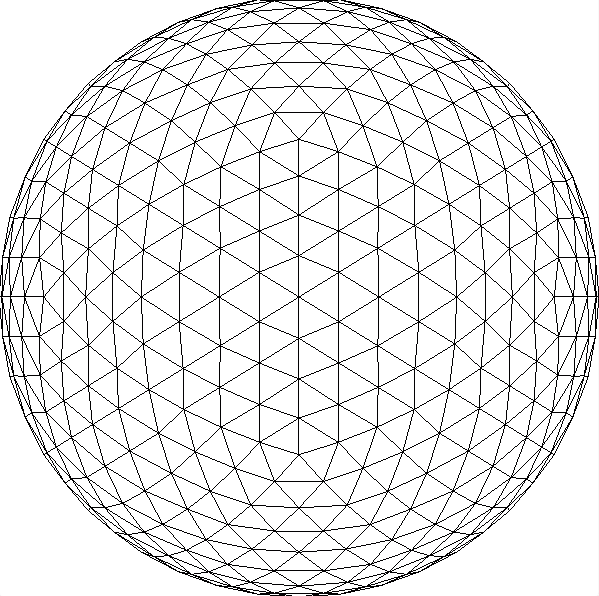
\includegraphics[width=.25\linewidth, angle=0]{figs/HARDI/Icosphere/icosphere_3.png}
    \label{fig::icosphere_3}
    }
    \hspace{1em}
    \subfloat[Tesselação de $16^a$ ordem]{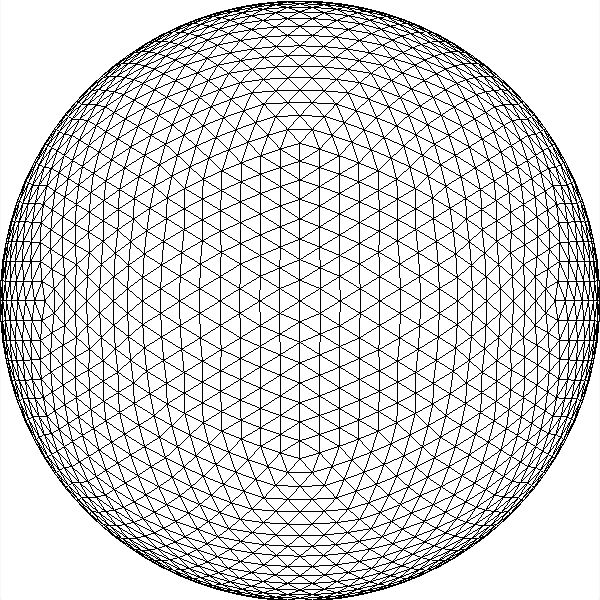
\includegraphics[width=.25\linewidth, angle=0]{figs/HARDI/Icosphere/icosphere_4.png}
    \label{fig::icosphere_4}
    }
     \caption{Esferas obtidas através da tesselação de um icosaedro.}
    \label{fig::icosphere}
\end{figure}

A quantidade de amostras em função da ordem de tesselação do icosaedro é dada por:

\begin{equation}
\label{eq::icosa_samples}
    N = 10\times t^2 + 2
\end{equation}

onde $t$ é a ordem de tesselação. A respeito das malhas esféricas mostradas na Fig. \ref{fig::icosphere}, a quantidade de vértices para $2^a$, $4^a$, $8^a$ e $16^a$ ordem de tesselação é 42, 162, 642 e 2562, respectivamente.

Seja o conjunto $\Pi = \{P_1, P_2, \dots, P_N\}$\footnote{Na Subseção \ref{ssec::geometria_base} do Capítulo \ref{chap::renderizacao_de_perfis_de_difusao}, sugerimos diretrizes para a formulação da estrutura de dados dos pontos de $\Pi$.} o conjunto de vértices da malha esférica obtida através da subdivisão do icosaedro. Para que possamos tomar vantagem da simetria de ODFs, condicionamos que $P_{2K+2} = -P_{2K+1}$ $(0 \leq K \leq \frac{N-2}{2})$.

Pode-se atribuir ao vetor $\mathbf{U} = [
\mathbf{n}_1, 
\mathbf{n}_2, ...,
\mathbf{n}_{N-1},
\mathbf{n}_N
]$, nos quais cada $\mathbf{n}_i$ é o vetor unitário na direção e sentido do vetor normal de $P_i$ ($P_i \in \Pi$), no entanto podemos tirar vantagem da simetria da ODF e reduzir o seu tamanho pela metade. Visto que os pontos simétricos em relação aos eixos da esfera tem normais em sentidos opostos, temos que $\mathbf{n}_{2K+2} = -\mathbf{n}_{2K+1}$, $(0 \leq K \leq \frac{N-2}{2})$. Observe que a função $\psi_m(\mathbf{r}, \mathbf{\hat{u}})$ (Eq. \ref{eq::sdf_discrete_2}) é simétrica em relação aos eixos em $\mathbf{\hat{u}}$, ou seja,  $\psi_m(\mathbf{r}, \mathbf{\hat{u}}) = \psi_m(\mathbf{r}, \mathbf{-\hat{u}})$, implicando que $\psi_m(\mathbf{r}, \mathbf{n}_{2K+2}) = \psi_m(\mathbf{r}, \mathbf{n}_{2K+1})$.

Assim, implementamos o cômputo das ODFs na quantidade metade das normais da esfera, o que permite que a quantidade de dados por \textit{voxel} seja diminuída pela metade em comparação a esfera inteira. Para isso, estabelecemos o vetor $\mathbf{U} = [
\mathbf{n}_1,
\mathbf{n}_3, ..., 
\mathbf{n}_{N-3},
\mathbf{n}_{N-1}
]$ de tamanho $S = N/2$, onde o vetor $\mathbf{\hat{u}}_K$ na K-ésima posição do vetor é dado por $\mathbf{n}_{2K-1}$ ($1 \leq K \leq S$). Assim, $\psi(\mathbf{r}, \mathbf{u}_K)$ é o valor de ODF no \textit{voxel} de índice $\mathbf{r}$ nas direções $\mathbf{n}_{2K-1}$, e também a direção $\mathbf{n}_{2K}$.

Recomendamos que a ordem de tesselação para amostragem seja a oitava ou, no máximo, a décima sexta, implicando em 321 e 1281 amostras de ODF por \textit{voxel}. Valores acima destes computados para todo DWI pode incorrer no uso de uma quantidade proibitiva de memória.

%Pode-se estabelecer que a estrutura de dados de $\mathbf{U}$ seja $[\mathbf{u_1}, \mathbf{u_2}, ..., \mathbf{u_{N-1}}, \mathbf{u_{N}}]^T$. Porém, podemos aproveitar a simetria dos dados e da malha esférica utilizada e organizarmos os dados de tal forma que um valor de ODF guardado na memória seja associado a duas direções simétricas.




\chapter{Renderização interativa de perfis de difusão}
\label{chap::renderizacao_de_perfis_de_difusao}

%\todo[inline]{Falta contextualizar nos objetivos que você listou na seção 1.3. Não é melhor focar em renderização de perfis de difusão que é um dos problemas relacionados diretamente com a interatividade?}

Neste capítulo, apresentamos o algoritmo de renderização interativa de ODFs através de glifos, integrado ao ambiente de visualização multimodal para visualização DWI. Mostraremos como resultados aspectos visuais, sua performance, na qual atestamos a sua interatividade.

A forma mais comum de visualizar dados derivados de ODFs é através glifos provenientes da superfície definida pela plotagem polar esférica $R(\mathbf{\hat{u}})$. Esta classe de superfície permite a inferência e inspeção de ODFs de difusão e sua distribuição de fibras subjacentes. Adicionalmente, permite a avaliação visual das ODFs obtidas a partir de um método HARDI para diferentes aquisições. Estes glifos dão uma visualização clara do comportamento local de difusão e são amplamente utilizados para provas de conceito em trabalhos na área de HARDI e essenciais para visualização dos resultados gerados pelos métodos avançados de imageamento.

Alguns dos exemplos de trabalhos que os utilizam, temos: \citeonline{TuchQBall2004} e \citeonline{yeh2010} os utilizam como ferramenta de visualização para o método de imageamento propostos em seus respectivos trabalhos; \citeonline{daducci2014} os utiliza para ilustrar e comparar ODFs reconstruídas por diferentes métodos; \citeonline{descoteaux2007}, para ilustrar transformações entre ODFs nos seus respectivos algoritmos de tractografia propostos. Isto evidencia que o algoritmo de renderização que estamos propondo não é restrito somente ao método GQI que apresentamos no Capítulo \ref{chapter::metodos_hardi}.

Este algoritmo de renderização, integrado a um sistema de visualização para DWI pode ser uma ferramenta poderosa para pesquisadores da área para avaliar perfis de difusão locais e melhorar o seu entendimento em métodos HARDI.

Adicionalmente, temos a conjectura que as ODFs representadas através de glifos posicionados em seus respectivos \textit{voxels} no ambiente de visualização multimodal pode melhorar o processo de escolha de parâmetros iniciais em tractografia. \citeonline{voltoline2021} trazem algumas evidências das circunstâncias que os superquádricos do DTI podem melhorar este processo, e conforme mostramos na Subseção \ref{ssec::aspectos_visuais}, mostramos que esses glifos são mais informativos que os superquádricos por permitir o inferimento do cruzamento de fibras.

O capítulo está organizado em 5 seções. Na Seção \ref{sec::glifos_odf} descreveremos a superfície e cor dos glifos, no qual chamaremos de glifos ODF; na Seção \ref{sec::trabalhos_relacionados}, apresentamos os trabalhos relacionados; na Seção \ref{sec::superquadricas}, apresentamos brevemente a \textit{pipeline} de renderização multimodal para superquádricos proposto por \citeonline{voltoline2021}; na Seção \ref{sec::renderizacao_de_glifos_ODF}, apresentamos a modificação na \textit{pipeline} da renderização multimodal para superquádricas e a nossa abordagem para renderização de glifos ODF; na Seção \ref{sec::experimentos}, mostramos a performance do esquema de renderização e aspectos visuais.

%\todo[inline]{Eu deixaria o parágrafo abaixo para conclusões}




%Esta classe de glifos são amplamente utilizados como uma ferramenta de visualização para prova de conceito em trabalhos na área de DWI. Além de \citeonline{TuchQBall2004}, alguns trabalhos relacionadosque os utilizam são: \citeonline{SCHILLING2019194}, para ilustrar a eficácia de métodos HARDI na detecção de direções de difusão, \citeonline{descoteaux2007}, para ilustrar o efeito de um\sout{a técnica} \todo{qual pré-processamento?}pré-processamento \sout{proposto} em ODFs que melhora a tractografia e \citeonline{yeh2010} 

%Foi implementado um esquema de visualização para ODFs em glifos de acordo através de representações gráficas polares esféricas. A implementação serviu primeiramente para prova de conceito e posteriormente otimizada para que seja possível a sua renderização, \textit{voxel} a \textit{voxel}, em tempo interativo pelo VMTK-Neuro, o que foi possível nos testes feitos em um Macbook Pro Retina 13', com processador Intel Core i5 Dual-Core 2.7Ghz, processador gráfico Intel Iris Graphics 6100 1536 MB e memória RAM de 8 GB 1867 MHz DDR3.

%\todo[inline]{Fazer uma breve justificativa da relevância da visualização das ODFs no contexto da sua proposta de uma visualização interativa almejando uma tractografia mais próxima dos tratos reais.}

\section{Glifos ODF}
\label{sec::glifos_odf}

%Como descrito na seção \ref{sec::trabalhos_relacionados_glifos}
\subsection{Superfície}

A superfície do glifo da ODF no voxel de coordenadas $\mathbf{r}$ $\psi(\mathbf{r}, \mathbf{\hat{u}})$ consiste na plotagem polar esférica onde $R(\mathbf{\hat{u}}) = \psi(\mathbf{r}, \mathbf{\hat{u}})$. A plotagem polar esférica $R(\mathbf{\hat{u}})$ é uma superfície na qual a distância da origem para um dos seus respectivos pontos na direção $\mathbf{\hat{u}}$ é dado por $R(\mathbf{\hat{u}})$.

% é dada por  na modulação do raio na direção $\mathbf{u}$ de uma esférica de acordo com uma versão normalizada do seu valor de imagem na função $\psi(\mathbf{u})$. A normalização que fizemos neste trabalho para representação está representado na equação \ref{eq::normglifo2}.

%\begin{equation}
%\label{eq::normglifo2}
%    R(\mathbf{u}) = \frac{\psi(\mathbf{u}) - min(\psi(\mathbf{u}))}{max(\psi(\mathbf{u})) - min(\psi(\mathbf{u}))}
%\end{equation}
\subsection{Cor}

As componentes r, g e b do mapeamento de cor esférica do glifo é dado em função da direção $\mathbf{\hat{u}} = (u_x, u_y, u_z)$, como definido em Eq. \ref{eq::cor_glifo} e ilustrado nos glifos da Fig. \ref{fig::glifo_ilustrado}. Esta forma de mapear, além de simples, é comumente utilizado pela comunidade DWI. %\todo{É imprescincível adicionar esta informação?}\sout{Não foi implementado o cômputo de vetores normais à superfície representadas pelo glifo, que consequentemente não tem iluminação associada.}

\begin{equation}
\label{eq::cor_glifo}
    r = |u_x| ~~~~ g = |u_y| ~~~~ b = |u_z|, 
\end{equation}

\begin{figure}[ht]

%\subfigcapskip = -5pt
    \centering
    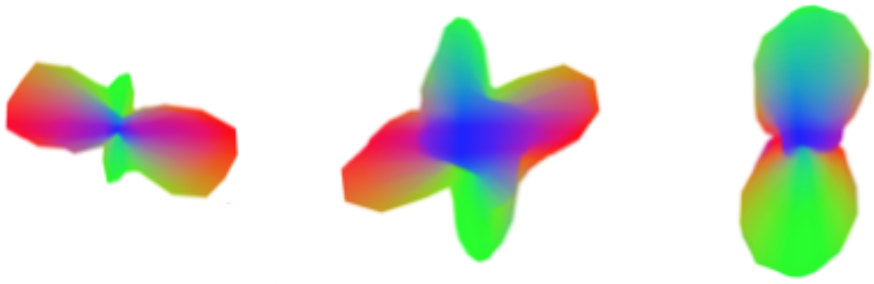
\includegraphics[width=.8\linewidth, angle=0]{figs/Esquema_Glifo/Glifos3Ex.png}
    \caption{Exemplos de glifos ODF. Os glifos consistem em uma superfície plotagem polar com a cor esquematizada de acordo com a equação \ref{eq::cor_glifo}.}
    \label{fig::glifo_ilustrado}
   \hspace{1pt}
\end{figure}

A respeito de planos anatômicos, a cor vermelha (r) representa a direção mediolateral, a verde (g), se refere a direção anteroposterior, e a azul (b), a direção inferior-superior.


\section{Trabalhos Relacionados}
\label{sec::trabalhos_relacionados}

Apesar da relevância reconhecida da renderização interativa de dados HARDI, a comunidade não tem explorado muito esta questão. Por questões de performance, nos limitaremos a trabalhos que exploram recursos da GPU. Há duas grandes abordagens achadas na literatura para renderização de glifos. A primeira é baseada em \textit{ray-casting}, onde a geometria do glifo é representada por uma função ou expressão algébrica \cite{peeters2009, almsick2011}. A outra é baseada na renderização de malhas, com a geometria do glifo aproximada por malhas poligonais \cite{shattuck2008}.

\citeonline{shattuck2008} tessela uma representação polar de ODF com triângulos, onde a superfície do glifo é gerada através da discretização do seu domínio polar, e sua forma é gerada na CPU através de uma função analítica neste domínio. Os glifos são renderizados por fatia. Com a mudança de malha e parâmetros de visualização, os vertices do glifo são re-computados e reenviados à GPU. A performance relatada é de dez \textit{frames}/s para uma fatia de um volume, no qual cada glifo tem 225 vértices, em uma cena com aproximadamente 2 milhões de triângulos. Neste trabalho, exploramos recursos da GPU modernos para melhorar a performance de renderização e seu uso de memória.


\citeonline{peeters2009} apresentaram um esquema de renderização utilizando \textit{ray-casting}. Na CPU, o centro, o raio da esfera delimitadora e o cubo delimitador por glifo são computados. Na GPU, o algoritmo de ray-casting é executdo por pixel no \textit{fragment shader}. Se o raio lançado para um pixel não intercepta a esfera delimitadora, o fragmento é descartado. Caso contrário, o algoritmo executa uma busca linear ,com passos discretos para interseção da ODF para com o raio. Eles alcançaram uma melhor performance que o algoritmo apresentado por \citeonline{shattuck2008}. \citeonline{almsick2011} melhorou a busca por interseção utilizando o método numérico \textit{regula falsi} e cilindros delimitadores alinhados com o eixo de visão. Eles atingiram um melhor tempo de performance sem sacrificar a qualidade de renderização, documentando que 9000 glifos puderam ser gerados a 30 FPS. Há um problema crítico na acurácia e eficiência do raio lançado. Quando o raio tende a ser paralelo ao glifo, muitas iterações podem ocorrer em algumas \textit{threads}. A renderização baseada em triângulos que propomos neste trabalho não apresenta este problema. 

\citeonline{voltoline2021} propuseram um esquema de renderização para glifos superquádricos para tensores de difusão \cite{Kindlmann2004}. Eles exploraram recursos modernos da GPU para atingir este objetivo, que consistem em \textit{transform feedback}, aproximação triangular adaptativa dos glifos e renderização por instanciação indireta. Diferentemente das superquádricas, os dados associados com glifos ODF tem dimensionalidade bem maior, o que inviabiliza seu armazenamento na GPU. Consequentemente, devemos propor estratégias para minimizar o tráfego de dados CPU-GPU para os glifos a serem renderizados, almejando a interatividade.

\section{Renderização multimodal de glifos superquádricas}
\label{sec::superquadricas}

\citeonline{voltoline2021} propuseram um algoritmo de renderização multimodal de glifos superquádricos sobre o seu respectivo MRI anatômico ponderado em T1. O volume $b0$, seu respectivo MRI T1 e a matriz rígida que co-registra ambos os volumes \cite{ting2014} são enviadas à GPU.

O algoritmo de renderização é dividido em três estágios: (1) renderização do DWI e do volume anatômico; (2) detecção dos \textit{voxels} visíveis e estimativa da cobertura máxima da projeção dos glifos em \textit{pixels}, para estimativa da resolução da malha; (3) renderização de \textit{voxels} visíveis na resolução estimada.

Para manter a compatibilidade do algoritmo com o Mac OSX, cuja versão máxima suportada do OpenGL é 4.1, eles desdobraram o algoritmo para estimação de cobertura máxima de \textit{pixels} para os glifos de um passo, onde a implementação é feita no \textit{compute shader} em um algoritmo de quatro passos, envolvendo \textit{vertex, geometry} e \textit{fragment shaders} baseados em rasterização. Para evitar transferência de dados entre CPU e GPU entre passos, o \textit{transform feedback buffer} foi aplicado. Adicionalmente, eles mostraram a utilização do mecanismo de \textit{additive blending} para obtenção do número máximo de \textit{pixels} ($max_p$), no qual o \textit{voxel} é projetado em um volume \textit{ray-casted}. Baseado em $max_p$, eles estabelecem uma heurística para estimação da resolução da malha.

Através de $max_p$, um \textit{tessellation shader} é acionado para gerar o \textit{skeleton} base dos superquádricos, no qual eles utilizam o comando renderização indireta por instâncias para desenhá-los com uma chamada desenho. Provendo a parâmetros particulares a cada \textit{voxel} que definem cada superquádrico, em cada instância o \textit{skeleton} é customizado para gerar o glifo e é posicionado em seu respectivo \textit{voxel} no espaço do volume.



\section{Renderização de Glifos ODF}
\label{sec::renderizacao_de_glifos_ODF}

Em nossa abordagem, o glifo é sintetizado pelo deslocamento dos pontos de uma malha esférica unitária base em função de $R(\mathbf{\hat{u}})$. Para uma malha esférica cujo conjunto de vértices é dado por $\{
P_1,
P_2, ...,
P_N
\}$, o glifo de uma ODF $R(\mathbf{\hat{u}})$ é gerado pelo escalonamento de cada um dos pontos $P_K$ da malha $(1 \leq K \leq N)$ pelo seu respectivo $R(\mathbf{n_K})$, onde $\mathbf{n_K}$ é o vetor unitário com direção e sentido da normal do ponto na esfera em $P_K$.


% A ODF associada a um \textit{voxel} é tipicamente representada por um conjunto de $N$ amostras de difusão $[
% R(\mathbf{\hat{n}}_1), 
% R(\mathbf{\hat{n}}_2), ...,
% R(\mathbf{\hat{n}}_{N-1}),
% R(\mathbf{\hat{n}}_N)
% ]^T$, onde cada $\mathbf{\hat{n}}_i$ é tem a direção e sentido da normal de cada ponto $ P_i$ de uma malha esférica. O glifo é sintetizado pelo deslocamento de cada ponto $P_i$ pelo seu escalar associado $R(\mathbf{\hat{n}}_i)$. Todas as amostras e ODF são computadas, conforme mostrado no Capítulo \ref{chapter::metodos_hardi} e acessíveis pelos seus respectivos ínndices de \textit{voxel}.


Devido a limitação de memória da GPU, aplicamos o algoritmo de detecção de \textit{voxels} visíveis \cite{voltoline2021} para obtermos um conjunto de $D = [
\mathbf{d}_1,
\mathbf{d}_2, ..., 
\mathbf{d}_M
]^T$ \textit{voxels} visíveis e sugerimos o envio à GPU das suas respectivas ODFs para renderização por instância, como ilustrado na Fig. \ref{fig::vmtk_simplified}. Este procedimento causa uma penalidade em performance devido ao tráfego de dados CPU-GPU devido as mudanças frequentes nas imagens renderizadas em função da interação com o usuário. Assim, nesta seção, apresentamos estratégias para enfrentar esta transferência afim de obter a renderização de forma interativa.

\begin{figure}[ht]
    \centering
    %\rule{6cm}{3cm}
    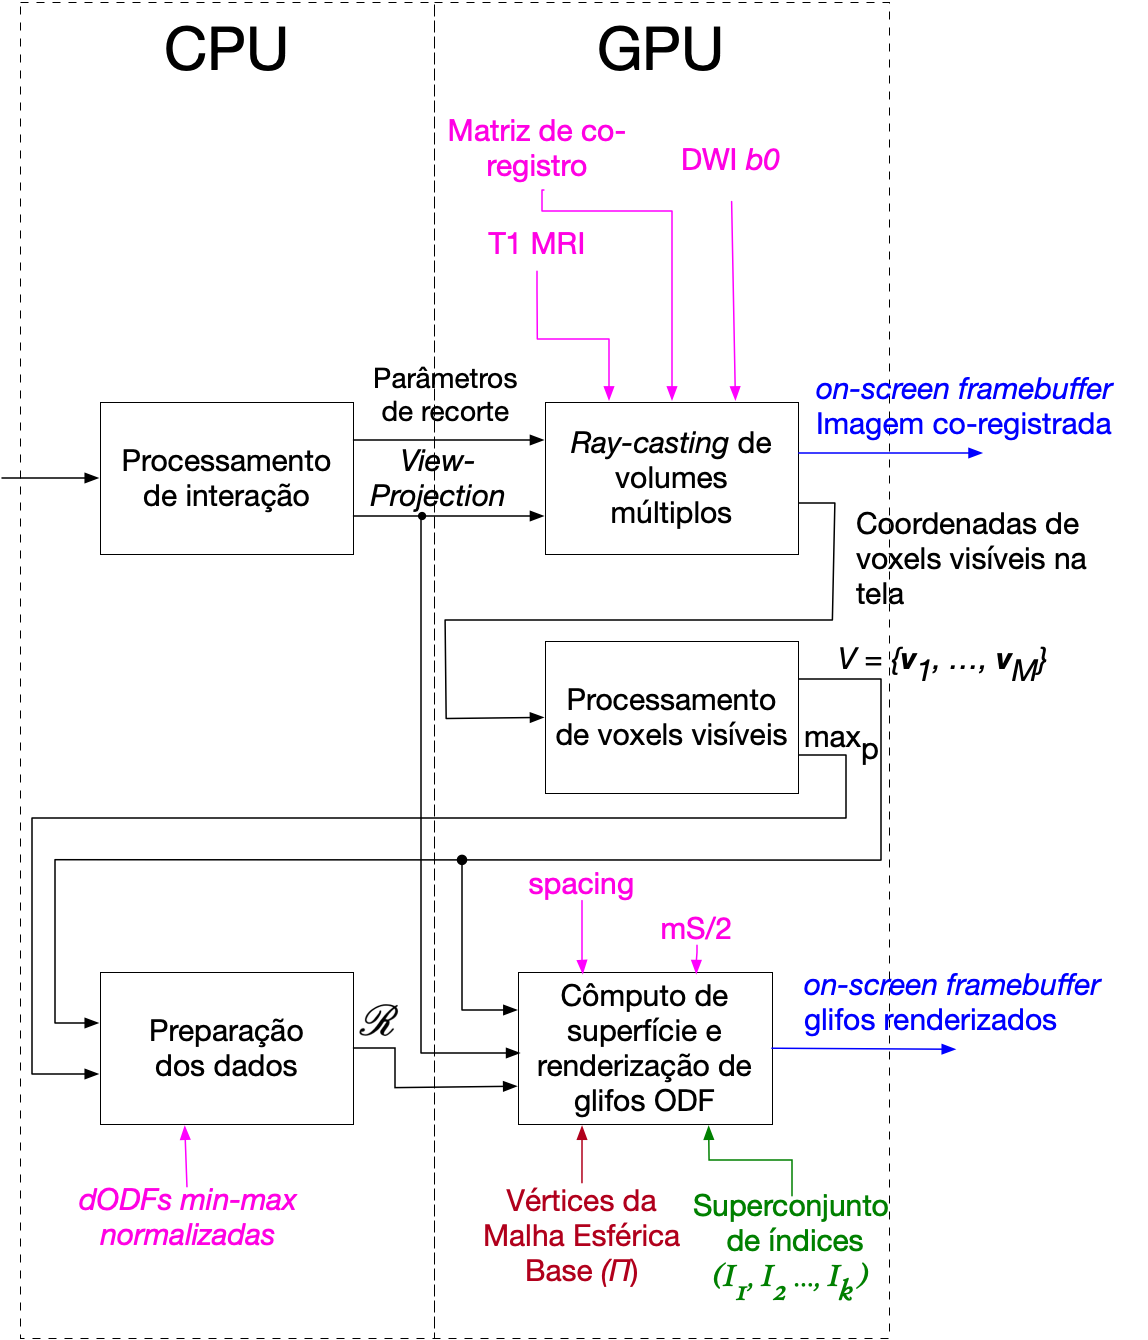
\includegraphics[width=.7\linewidth, angle=0]{figs/Esquema_Glifo/fluxograma_glifos_VMTK.png}
    \caption{
    Renderização multimodal para glifos ODF. A cor azul representa a saída a ser desenhada, armazenada no \textit{framebuffer} (FB); a cor magenta se refere a dados pré-computados. Os estágios de \textit{raycasting} do volume e processamento de \textit{voxels} visíveis estão descritos por \citeonline{voltoline2021}. O estágio de preparação dos dados de ODF e renderização de glifos ODF estão descritos na Seção \ref{sec::renderizacao_de_glifos_ODF}.
    }
    \label{fig::vmtk_simplified}
\end{figure}

Nossa solução para minimizar a transferência de dados consiste em explorar a resolução da percepção visual, o uso de renderização por instâncias, exploração da simetria de ODFs e o uso de memória de textura. Na Subseção \ref{ssec::geometria_base}, descrevemos a geometria base que é deformado por cada conjunto de amostras de ODF. Na Subseção \ref{ssec::atributos}, descrevemos o leiaute de atributos que otimiza o uso de memória da GPU e o seu acesso.

\subsection{Geometria base}
\label{ssec::geometria_base}

\subsubsection{Considerações iniciais}

As ODFs são amostradas a partir dos vetores normais dos pontos de uma malha base esférica $(\Pi, I)$, onde $\Pi = [P_1, P_2, \dots, P_N]$ consiste num conjunto de pontos não repetidos e o conjunto $I$ são os índices que referenciam os pontos de $\Pi$ para formar os triângulos que sintetizam a malha. Estabelecemos duas condições para a estrutura de dados, nas quais tiramos proveito da simetria de dados das ODFs e para que façamos a malha ser adaptativa para parâmetros de visualização. Estas condições tem impacto direto no tráfego de dados CPU-GPU, conforme discutido na Subseção \ref{ssec::atributos}.

A primeira condição, conforme já discutido no capítulo \ref{chapter::metodos_hardi} na forma de armazenamento de dados da ODF tira vantagem da simetria e armazena os pontos em metade de uma esfera. Propomos que os pontos simétricos em relação aos eixos coordenados de $\Pi$ estejam dispostos de forma consecutiva na memória, i. e. $P_{2i+2} = -P_{2i+1}$, $(0 \leq i \leq \frac{N-2}{2})$, o que nos leva a uma estrutura de dados $\Pi = [P_1, -P_1, P_3, -P_3, \dots, P_{N-3}, -P_{N-3}, P_{N-1}, -P_{N-1}]^T$.

A segunda condição objetiva fazer a geometria base do glifo ser adaptativa como uma sub-malha da malha esférica base. Seja $k$ o número de sub-malhas de $(\Pi, I)$, onde cada sub-malha é denotada por $(\Pi_i, I_i)$,  $(0 \leq i < k)$, adicionalmente, o número de pontos das sub-malhas é crescente de acordo com os sub-índices, i.e. se $(0 \leq i < j < k)$, implica $|\Pi_j| > |\Pi_i|$. Sugerimos que cada sub-malha $(\Pi_i, I_i)$ seja simétrica em relação a origem e os primeiros $|\Pi_i|$ elementos na estrutura de dados de $\Pi$ corresponda aos elementos de $\Pi_i$. Note que esta condição também implica que, para $i$, $j$ tais $0 \leq i < j < k$, $\Pi_i$ é subconjunto de $\Pi_j$.

\subsubsection{Formulação da geometria e estruturação de dados}

Conforme mencionado no capítulo \ref{chapter::metodos_hardi}, escolhemos o conjunto de malhas derivada da $2^k$-ésima ordem de tesselação do icosaedro. O algoritmo para obtermos a tesselação de $2^k$-ésima ordem é um processo iterativo repetido $k$ vezes que se inicia com o icosaedro. Cada triângulo da malha é subdividido em quatro em cada iteração, onde os novos novos vértices adicionados são computados pela projeção da mediana dos pares de pontos conectados por uma aresta na esfera. Assim, o conjunto de vértices da $2^k$-ésima ordem contém todos os vértices das iterações anteriores. Adicionalmente, são todos simétricos com relação a origem. O processo de subdivisão de um triângulo está ilustrado na Fig. \ref{fig::triangle_icosahedron} e o algoritmo para se obter esta categoria de malha pode ser encontrado em \citeonline{luna2012}. Adicionalmente, a Fig. \ref{fig::icosphere} do Capítulo \ref{chapter::metodos_hardi} ilustra malhas esféricas desta categoria.

\begin{figure}[htb]
    \centering
    %\rule{6cm}{3cm}
    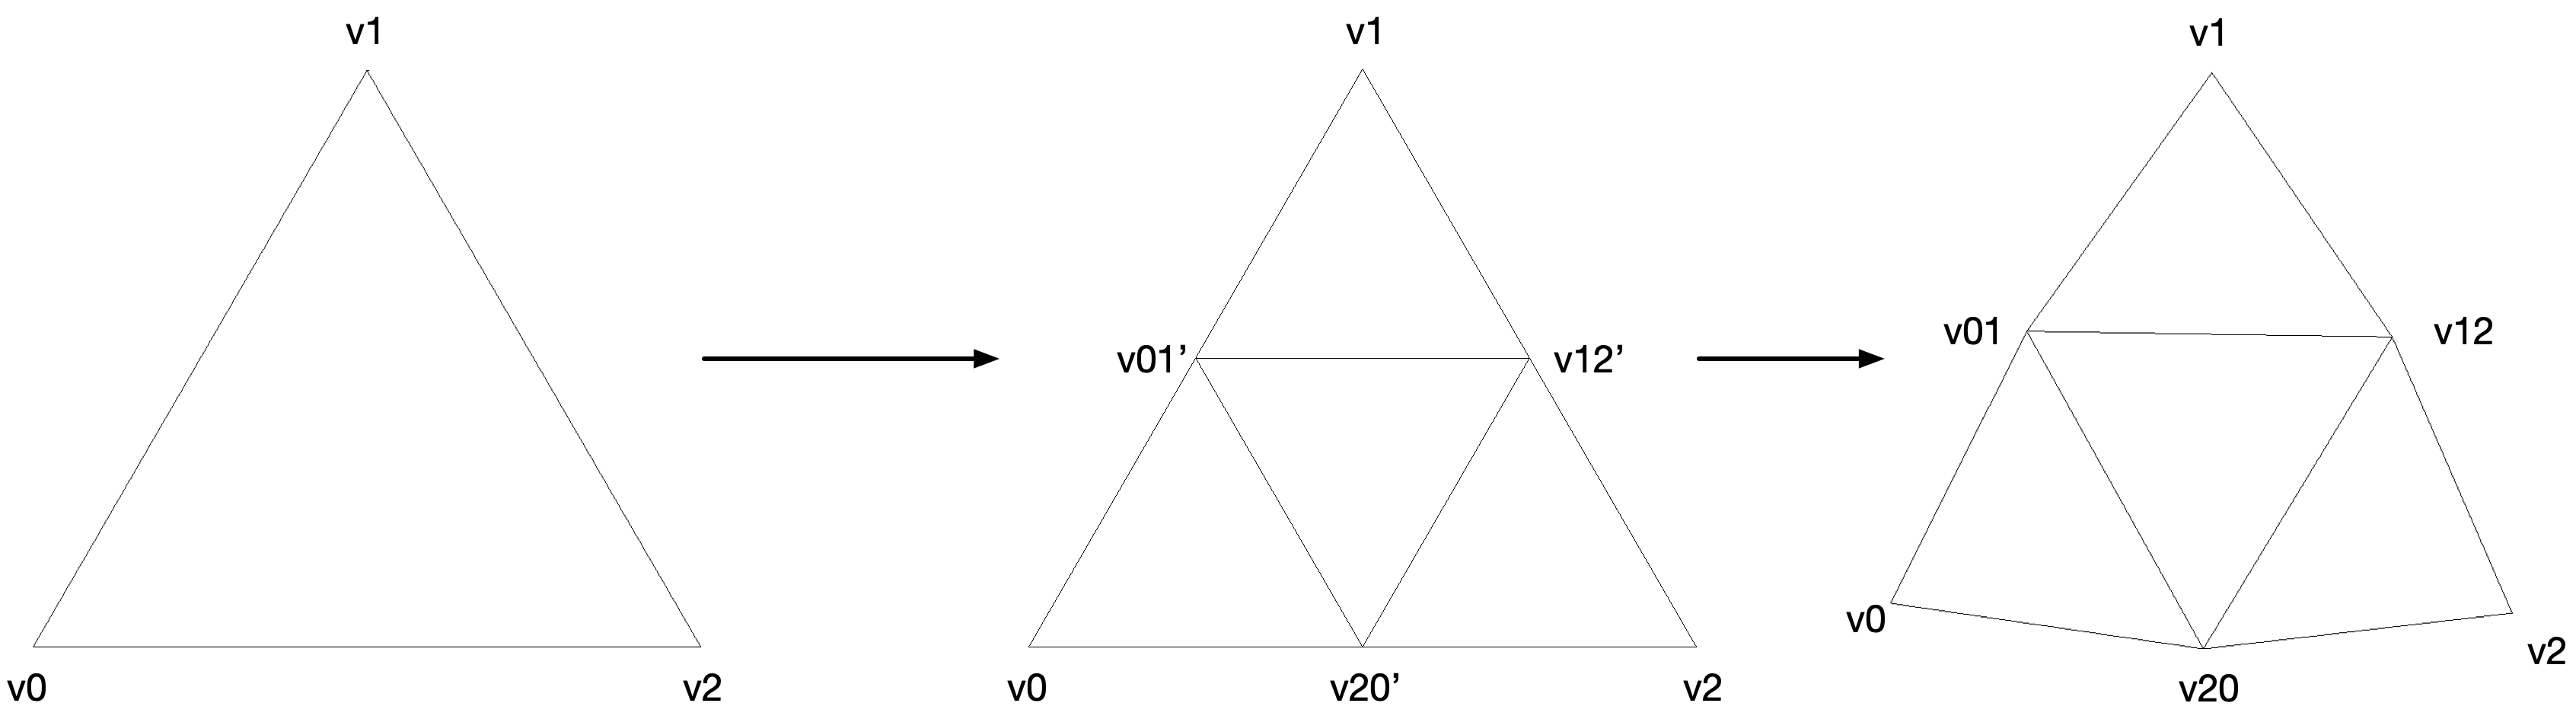
\includegraphics[width=1.0\linewidth, angle=0]{figs/Esquema_Glifo/ico_subdivision.png}
    \caption{
    Subdivisão de um triângulo para formar quatro na formação da malha esférica a partir da tesselação de $2^k$-ésima ordem a partir da partir da $2^{k-1}$-ésima. O triangulo formado pelos vértices $v0$, $v1$ e $v2$ é subdividido em quatro, onde as medianas  $v01'$, $v12'$ e $v20'$ são computadas e suas respectivas projeções na esfera $v01$, $v12$ e $v20$ são adicionados ao conjunto de vértices.
    }
    \label{fig::triangle_icosahedron}
\end{figure}

Há dois problemas adicionais que precisamos enfrentar no que diz respeito a obtenção de malhas esféricas através da subdivisão do icosaedro. O primeiro é garantir que os vértices simétricos estejam de forma consecutiva na memória e o segundo diz respeito a que não haja repetição de pontos em $\Pi$. O algoritmo para subdivisão do icosaedro em \citeonline{luna2012} insere vértices repetidos, pois há diversos pares de pontos conectados que definem mais de um triângulo.

A nossa abordagem para resolver esse problema consiste em identificar e deletar pontos replicados para termos somente uma amostra de cada em $\Pi$ e, após isso, ordenar o conjunto de dados $\Pi$ para que os simétricos estejam de forma consecutiva na memória, e essa mudança de estrutura de dados tem que ser compensada no conjunto de índices $I$. Para resolver estes problemas, propomos dois algoritmos que resolvem essas questões de forma genérica que são executados após cada iteração da subdivisão do icosaedro. O Algoritmo \ref{alg::tira_redundancia_pontos} certifica que os pontos redundantes são removidos, e o Algoritmo \ref{alg::reordena_simetricos} certifica que os pontos simétricos estarão em sequência na memória.

\begin{algorithm}
\caption{Algoritmo para retirada de pontos repetidos em estrutura de dados de vértices}
\label{alg::tira_redundancia_pontos}
\begin{algorithmic}[1]
\Procedure{ShrinkVertexSet}{$\Pi$, $I$}
 \State $I' \gets [0, 1, 2, ..., |\Pi| - 1]$
\State $i \gets 0$
\While{$i < |\Pi| - 1$} \label{alg::svs_pt1_inicio}
    \State $j \gets i + 1$
    \While{$j < |\Pi|$}
        \If {$\Pi[i] = \Pi[j]$}
            \State $I'[j] \gets i$
        \EndIf
        \State $j \gets j + 1$
    \EndWhile
    \State $i \gets i + 1$
\EndWhile \label{alg::svs_pt1_fim}
\State $\Pi_{size} \gets |\Pi|$
\State $i \gets 0$
\While{$i < \Pi_{size} - 1$} \label{alg::svs_pt2_inicio}
    \State $j \gets i + 1$
    \While{$j < \Pi_{size}$}
        \If{$\Pi[i] = \Pi[j]$}
            \State DELETE $\Pi[j]$ \label{alg::delete}
            \ForEach{$c \in I'$ \textbf{and} $c > j$}
                \State $c \gets c - 1$
            \EndFor
            \State $j \gets j - 1$
            \State $\Pi_{size} \gets \Pi_{size} - 1$
        \EndIf
        \State $j \gets j + 1$
    \EndWhile
    \State $i \gets i + 1$
\EndWhile \label{alg::svs_pt2_fim}
\ForEach{$c \in I$} \label{alg::resetI}
    \State $c \gets I'[c]$
\EndFor
\EndProcedure
\end{algorithmic}
\end{algorithm}

 \begin{algorithm}
 \caption{Pseudocódigo que sequencia vértices simétricos na memória}
 \label{alg::reordena_simetricos}
 \begin{algorithmic}[1]
 \Procedure{AlignSymmetricalMesh}{$\Pi$, $I$}
 \State $I' \gets [0, 1, 2, ..., |\Pi| - 1]$
 \State $i \gets 0$
 \While{$i < |\Pi| - 1$} 
     \State $j \gets i + 1$
     \While{$j < |\Pi|$}
         \If {$\Pi[i] = -\Pi[j]$}
             \State Swap($\Pi[i+1]$, $\Pi[j]$) \label{alg::troca}
             \ForEach{$c \in I$} \label{alg::compensacao_inicio}
                \If{$c = i+1$}
                    \State $c \gets j$
                \ElsIf{$c = j$}
                    \State $c \gets i+1$
                \EndIf
             \EndFor
             \State \textbf{break}
         \EndIf 
         \State $j \gets j + 1$
         \If {$j = |\Pi|$}
            \State \textbf{return} ERROR\_MESH\_NOT\_SYMMETRICAL
         \EndIf
     \EndWhile \label{alg::compensacao_fim}
     \State $i \gets i + 2$
\EndWhile
 \EndProcedure
 \end{algorithmic}
 \end{algorithm}
 
 O Algoritmo \ref{alg::tira_redundancia_pontos} pode ser dividido em duas partes e tem no vetor $I'$ o seu ponto crucial de funcionamento. Cada $I'[i]$ armazena está associado ao $i$-ésimo elemento de $\Pi$. Após a deleção dos elementos repetidos em $\Pi$, $I[i]$ guarda o índice do ponto que é igual a $\Pi[i]$ antes da deleção dos vértices repetidos.
 
 A primeira parte do algoritmo (Linhas \ref{alg::svs_pt1_inicio} até \ref{alg::svs_pt1_fim}) consiste trocar os vértices repetidos apontados por $I'$ para a sua primeira ocorrência em $\Pi$, visto que as demais ocorrências irão ser apagadas. A segunda parte do algoritmo (Linhas \ref{alg::svs_pt2_inicio} até \ref{alg::svs_pt2_fim}) consiste na deleção dos vértices repetidos, o comando DELETE na linha \ref{alg::delete} considera que a o processo de deleção do elemento consiste em deslocar os seus elementos conseguintes na memória para o endereço anterior\footnote{O funcionamento descrito é similar à função std::erase aplicada a classe std::vector em C++}, consequentemente, isto é compensado no conjunto de índices $I'$ pelo decremento de todos os índices apontados com valores maiores do que $j$. Na linha \ref{alg::resetI}, o elementos no conjunto de índices $I$ são corrigidos para referenciar para nova versão sem redundância de $\Pi$.
 
O Algoritmo \ref{alg::reordena_simetricos}, consiste na detecção dos simétricos e a troca de posição de pontos em índices ímpares para os simétricos dos índices pares em $\Pi$ (Linha \ref{alg::troca}) na posição anterior e a compensação no conjunto de índices $I$ (Linhas \ref{alg::compensacao_inicio} até \ref{alg::compensacao_fim}).

Sendo assim, o Pseudocódigo \ref{alg::setIcosahedroBase} mostra os procedimentos para subdivisão do icosaedro, bem como onde os algoritmos \ref{alg::tira_redundancia_pontos} e \ref{alg::reordena_simetricos} se situam. A variável $k$ representa a quantidade de iterações, $\mathbf{I}$ é o superconjunto que contém os conjuntos de índices para diferentes resoluções do glifo e $\Pi$ a lista de vértices do icosaedro tesselado de ordem $2^k$.

Na linha \ref{alg::subdivide_icosahedron}, temos o algoritmo de subdivisão dos triângulos em quatro \cite{luna2012}, obtidos como ilustrado na Fig. \ref{fig::triangle_icosahedron}, adicionalmente, os novos vértices gerados são alocados após o fim da estrutura de dados dos vértices base, o que faz com que, os vértices do icosaedro estejam situados no início da estrutura, seguidos dos vértices gerados pela primeira subdivisão, depois dos vértices gerados na segunda subdivisão e assim sucessivamente.

 \begin{algorithm}
 \caption{Pseudocódigo que gera diferentes esferas a partir de tesselações de ordem $2^k$ do icosaedro.}
 \label{alg::setIcosahedroBase}
 \begin{algorithmic}[1]
 \Function{SetIcosahedronSet}{$k$}
 \State $\mathbf{I} = \{I_0, I_1, ..., I_{k-1}, I\}$
 \State $(\Pi, I) = \text{(Icosahedron.Vertices, Icosahedron.Indices)}$  \cite{luna2012} \label{alg::init_icosahedron}
 \State $i \gets 0$
 \While{$i < k$}
    \State ShrinkVertexSet($\Pi, I$)
    \State AlignSymmetricalMesh($\Pi, I$)
    \State $I_i \gets I$
    \State ($\Pi$, $I$) = SubdivideTriangles($\Pi, I$) \cite{luna2012}  \label{alg::subdivide_icosahedron}
    \State $i \gets i + 1$
\EndWhile
    \State \textbf{return} $(\Pi, \mathbf{I})$
 \EndFunction
 \end{algorithmic}
 \end{algorithm}
 

Assim, definindo $(\Pi, I)$ para ser a $2^{k}$-ésima ordem de tesselação para ser a malha esférica base e mantendo cada conjunto de índices de menor ordem a cada iteração, temos um conjunto de $k$ sub-malhas $(\Pi_0, I_0), (\Pi_1, I_1), ..., (\Pi_{k-1}, I_{k-1})$ definidos como as tesselações de $1^{a}$, $2^{a}$, ... $2^{k-1}$-ésima ordem. As Eq. \ref{eq::2ordem_icosphere_vertices}\footnote{Note que esta equação é a Eq. \ref{eq::icosa_samples} adaptada para $2^k$-ésima ordem de tesselação do icosaedro} e \ref{eq::2ordem_icosphere_triangulos} computam a quantidade de vértices e triângulos para esta categoria de malha em função da tesselação de ordem $2^k$, respectivamente.

\begin{equation}
\label{eq::2ordem_icosphere_vertices}
V = 10\times 4^k + 2
\end{equation}

\begin{equation}
\label{eq::2ordem_icosphere_triangulos}
\tau = 20\times 4^k
\end{equation}

Assim como mencionado no capítulo \ref{chapter::metodos_hardi}, por questões de memória, recomendamos k = 3, ou no máximo 4. Assim, formulamos a estrutura de dados que satisfaz as duas condição que estabelecemos a princípio, e é tal que os primeiros 12 elementos correspondem aos vértices do icosaedro, os 42 primeiros elementos correspondem aos vértices da $2^a$ ordem de tesselação, os 162 primeiros elementos correspondem a $4^a$ ordem de tesselação, os primeiros 642 elementos correspondam a $8^{a}$ ordem de tesselação, e, adicionalmente, os pontos simétricos são agrupados em sequencia na memória.

A estrutura de dados $\Pi$, e $I$, além dos índices que triangulam todas as sub-malhas, contidos ao superconjunto $\mathbf{I}$ no Algoritmo \ref{alg::setIcosahedroBase}, são enviados à GPU uma vez. Uma vez que os dados estão na GPU, e visando eficiência no processamento, sem comprometer a qualidade visual, escolhemos adaptativamente a geometria base entre estas malhas por um procedimento heurístico computado em tempo de execução baseado em $max_p$.

\subsubsection{Escolha automática da geometria base}

A escolha da geometria base é baseada no \textit{trade-off} de \citeonline{voltoline2021}, que indica a quantidade mínima de triângulos para dado um $max_p$, que é dado por $\tau \geq 8\sqrt{max_p}$  ($max_p > 0$). Este \textit{trade-off} estabelece a quantidade mínima de triângulos a ser utilizada na malha que não sacrifica a qualidade de imagem dos glifos. Derivamos uma expressão para a escolha da sub-malha da malha esférica base a partir do caso de igualdade do \textit{trade-off}, no qual substituímos a quantidade de triângulos como uma função da ordem de tesselação do icosaedro e mapeamos o icosaedro para o caso $max_p = 0$. A expressão base está na Eq. \ref{eq::icosa_order_base}:

\begin{equation}
\label{eq::icosa_order_base}
     20\times 4^k - 20\times 4^0 = 8\sqrt{max_p}
\end{equation}

Derivamos $t$ ($t \leq k$) na Eq. \ref{eq::icosa_order} como a ordem de tesselação do icosaedro escolhida. Como $t$ é inteiro positivo, para satisfazer o \textit{trade-off} de \citeonline{voltoline2021}, arrendondamos o valor para cima.

\begin{equation}
\label{eq::icosa_order}
     t = \lceil \frac{1}{2}\log_2{(\frac{2}{5}\sqrt{max_p} + 1)} \rceil
\end{equation}

Para geometria base derivada da $2^t$-ésima ordem de tesselação, devemos ser atentos a dois procedimentos na seleção da malha em tempo de execução. O primeiro consiste na ativação do seu respectivo conjunto de índices para triangulação. O segundo consiste em setar a quantidade de dados de ODF por glifo enviado à GPU como uma função de sua quantidade de vértices, o que será discutido mais a frente, na Subseção \ref{ssec::atributos}.


\subsubsection{Fator de escala para geometria}

Finalmente, sugerimos escalar a a malha base pelo fator de escala $mS$ para proporcionar a máxima ocupância em tela, fazendo o glifo, cuja ODF está contida no intervalo $[0, 1]$, caber no seu respectivo \textit{voxel}:

\begin{equation}
\label{eq:spacings}
mS = min(spacing_x, spacing_y, spacing_z)
\end{equation}


onde $spacing_x$, $spacing_y$, $spacing_z$ é o espaço entre duas amostras adjacentes nos eixos x, y e z, respectivamente.





%The vertices and amount of triangles and the expression for the vertices and triangles number for each $2^k$ tessellation are in Table \ref{tab::icosahedron_set}. In practice, we recommend $k$ to be equal to 3 or 4, at most. Values of above those may incur a prohibitive amount of memory for pre-computed ODF samples in a DWI.




\subsection{Atributos}
\label{ssec::atributos}



Para renderizarmos $M$ glifos com um comando de desenho, usamos instanciação de GPU. A geometria base selecionada, referente a $2^t$-ésima ordem de tesselagem do icosaedro é instanciada por um vetor de translação e amostras de ODF.

\subsubsection{Posicionamento}

Para $M$ \textit{voxels} visíveis, enviamos os vetores de translação como um atributo por instância, que é computado em função das coordenadas de \textit{voxel} $V(v_x, v_y, v_z)$ como:

\begin{align}
 \label{eq::translation}
    dx = (v_x + 0.5).spacing_x \nonumber\\
    dy = (v_y + 0.5).spacing_y \\
    dz = (v_z + 0.5).spacing_z \nonumber
\end{align}

Note que os dados de voxel visíveis retornados pelo algoritmo é armazenado em um buffer na GPU. Este dado é utilizado diretamente no algoritmo de renderização no \textit{vertex shader} para cômputo do atributo de translação.

\subsubsection{Dados de ODF}

Como mencionado no capítulo \ref{chapter::metodos_hardi}, aproveitamos a simetria dos dados de ODF para organizarmos os dados no domínio de um hemisfério. Para o voxel de coordenandas índice $\mathbf{r}$, os elementos são organizados como $\boldsymbol{\psi} = [
\psi(\mathbf{r}, \mathbf{n}_1),
\psi(\mathbf{r}, \mathbf{n}_3), ...,
\psi(\mathbf{r}, \mathbf{n}_{N-3}),
\psi(\mathbf{r}, \mathbf{n}_{N-1})]^T$. Onde cada elemento na K-ésima posição $\psi(\mathbf{r}, \mathbf{n}_{2K-1})$ desloca os pontos $P_{2K-1}$ e seu simétrico $P_{2K}$ na geometria base instanciada. Note que no capítulo \ref{chapter::metodos_hardi}, o armazenamento de amostras em metade de uma esfera tem o objetivo de economia de memória, enquanto neste capítulo, tem o objetivo de minimizar o tráfego de dados CPU-GPU.

Para a geometria base escolhida, geramos uma matriz com os dados de ODF enviados à GPU como a matriz $\mathbf{R}_{\frac{V}{2}xM}$ (Eq. \ref{eq::R}), onde $V$ é o numero de vértices da geometria base, dado por $10 \times 4^t + 2$ (Eq. \ref{eq::2ordem_icosphere_vertices}). A $j$-ésima coluna consiste nos primeiros $V/2$ elementos de $\boldsymbol{\psi}(\mathbf{d_j})$. $\mathbf{R}$ é enviado à GPU como uma textura 2D de formato RGBA.

\begin{equation}
\label{eq::R}
\mathbf{R} = 
\begingroup % keep the change local
\setlength\arraycolsep{2pt}
\begin{bmatrix} 
    \psi(\mathbf{d}_{1}, \mathbf{n}_1) &
    \psi(\mathbf{d}_{2}, \mathbf{n}_1) & \cdots & 
    \psi(\mathbf{d}_{M}, \mathbf{n}_1)  \\
    
    \psi(\mathbf{d}_{1}, \mathbf{n}_3) &
    \psi(\mathbf{d}_{2}, \mathbf{n}_3) & \cdots & 
    \psi(\mathbf{d}_{M}, \mathbf{n}_{3}) \\ \vdots & \vdots & \vdots & \vdots  \\
    
    \psi(\mathbf{d}_{1}, \mathbf{n}_{V-1}) & 
    \psi(\mathbf{d}_{2}, \mathbf{n}_{V-1}) & \cdots & 
    \psi(\mathbf{d}_{M}, \mathbf{n}_{V-1})
\end{bmatrix}.
\endgroup
\end{equation}

Cada \textit{texel} no formato RGBA suporta quatro valores. Agrupamos os valores escalares da j-ésima coluna $[
\psi(\mathbf{d}_{j}, \mathbf{n}_1),
\psi(\mathbf{d}_{j}, \mathbf{n}_3), ...,
\psi(\mathbf{d}_{j}, \mathbf{n}_{V-3}),
\psi(\mathbf{d}_{j}, \mathbf{n}_{V-1})
]^T$ de quatro em quatro, como mostrado na Fig. \ref{fig::texelfetch}. Consequentemente, em cada acesso de \textit{texel}, temos quatro valores escalares $
\psi(\mathbf{d}_{j}, \mathbf{\mathbf{n}_{8K+1}})$ (R), $
\psi(\mathbf{d}_{j}, \mathbf{\mathbf{n}_{8K+3}})$ (G), $
\psi(\mathbf{d}_{j}, \mathbf{\mathbf{n}_{8K+5}})$ (B), $
\psi(\mathbf{d}_{j}, \mathbf{\mathbf{n}_{8K+7}})$ (A). Nos quais deslocamos quatro pares de pontos simétricos na geometria base $P_{8K+1}$, $-P_{8K+1}$, $P_{8K+3}$, $-P_{8K+3}$, $P_{8K+5}$, $-P_{8K+5}$, $P_{8K+7}$, $-P_{8K+7}$ para o j-ésimo glifo visível (também j-ésima instância). Desta forma, as dimensões da textura com dados ODF é $ \frac{V/2}{4} \times M$. Se $\frac{V}{2}$ não é divisível por quatro, é necessário inserir mais linhas abaixo da última com valores \textit{dummy}, para que o número de linhas se torne divisível, o que certifica que cada coluna de $\mathbf{R}$ possa ser acessada com o índice de instância na GPU.

\begin{figure}[ht]
%\subfigcapskip = -5pt
    \centering
    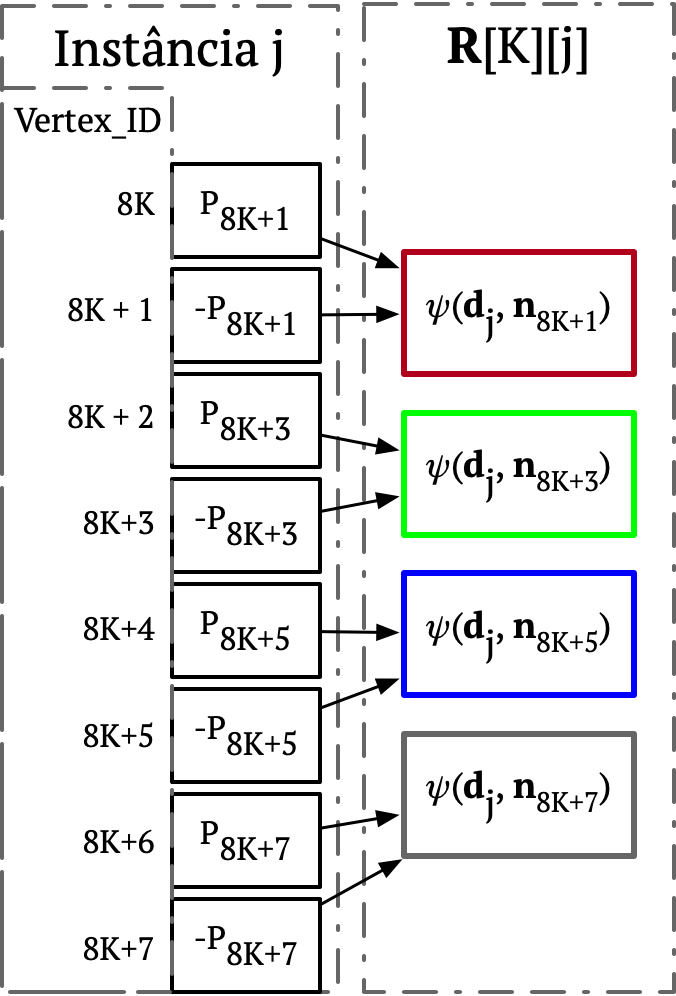
\includegraphics[width=.45\linewidth, angle=0]{figs/Esquema_Glifo/texellookup.png}
    \caption{Ilustração do acesso nas componentes RGBA em \textit{texel} na textura \textbf{R} no índice $K$ e $j$. O \textit{texel} é acessado pelas threads que processam os vertices de índices 8K, 8K+1, ..., 8K+7 em uma instância $j$. Os blocos de contorno vermelho, azul, verde e cinza ilustram as componentes R,G,B e A do \textit{texel}, respectivamente.}
    \label{fig::texelfetch}
   %\hspace{1pt}
\end{figure}

Os dados de ODF são acessados no \textit{vertex shader}, quando cada glifo da $j$-ésima instância é processada. Os \textit{texels} com índice de coluna $K = \lfloor\frac{Vertex\_ID}{8} \rfloor$ são acessados para deslocar oito pontos. Usamos a função \textit{texelFetch} para acessar diretamente a textura de ODF utilizando coordenadas não-normalizadas $(j, \lfloor\frac{Vertex\_ID}{8} \rfloor)$. O valor utilizado para \textit{lookup} da componente  para deslocar o seu respectivo ponto na geometria base no \textit{vertex shader} é acessível pela análise do resto da divisão por oito do Vertex\_ID, como ilustrado na Fig. \ref{fig::texelfetch}. Adicionalmente, utilizando a notação via colchetes, onde as componentes R, G, B e A são mapeados nos índices 0, 1, 2 e 3, respectivamente, o escalar de ODF pode ser mapeado por $\lfloor (Vertex\_ID \mod{8})/2 \rfloor$\footnote{A função em OpenGL para \textit{lookup} em função dos índices de instância e vértice é dada por texelFetch($\mathbf{R}$,ivec2((gl\_VertexID)/8, gl\_InstanceID), 0)[(gl\_VertexID\%8)/2]}.

\subsection{Síntese}

Podemos sintetizar as transformações aplicadas a cada vértice $P_K$ em coordenadas homogêneas na $j$-ésima instância por uma multiplicação matricial no \textit{vertex shader} por uma matriz $G_{Kj}$. Esta matriz pode ser sintetizada da seguinte forma:

\begin{equation}
    G_{Kj} = \mathbf{M_{vp}}\cdot M_D \cdot M_S \cdot M_{Kj}
\end{equation}

onde $M_{kj}$ é a matriz que escalona o ponto $P_K$ na $j$-ésima instância por $\psi(\mathbf{d}_j, \mathbf{n}_k)$, $M_S$ se refere a transformação de escala, dado por Eq. \ref{eq:spacings}, $M_D$ é a matriz de translação do glifo, centrado na origem para o centro do seu respectivo \textit{voxel} no espaço do volume, dado pela Eq. \ref{eq::translation}, e, adicionalmente, $\mathbf{M_{vp}}$ é a matriz \textit{view-projection}, que configura parâmetros de visão e projeção.

\section{Experimentos, resultados e discussão}
\label{sec::experimentos}

Propomos um experimento para avaliar aspectos visuais do nosso algoritmo de esquema de renderização em comparação à superquádricas e medições de performance para atestarmos a interatividade do algoritmo de renderização. Os tempos de medição foram feitos em um computador Macbook Pro Retina 13', com processador Intel Core i5 Dual-Core 2.7GHz, processador gráfico integrado Intel Iris Graphics 6100 1536 MB e memória RAM de 8 GB 1867 MHz DDR3.

As imagens geradas no experimento foram coletadas a partir o WU-Minn HCP Retest Data pelo \textit{Connectome Project Consortium} \cite{essen2012}.

Os dados de difusão foram adquiridos em um \textit{scanner} Siemens 3T Skyra. A aquisição é \textit{multi-shell} com 90 gradientes de ponderação de difusão para cada $b = 1000, 2000$ e $3000 s/mm^2$, e estas direções são uniformemente distribuídas nos três \textit{shells}, e adicionalmente foram escaneados 6 aquisições $b0$ para cada \textit{shell}, totalizando 288 imagens. Os dados foram pré-processados com a \textit{pipeline} de pré-processamento para dados de difsão do Human Connectomme Project (HCP) \cite{glasser2013}. A aquisição pré-processada é representada por um volume $145\times 174\times  145$ com espaço entre amostras de $1.25\times 1.25 \times 1.25$mm.

A aquisição anatômica ponderada em T1 foi também pré-processada utilizando a pipeline de pré-processamento do HCP \cite{glasser2013}. Como o seu respectivo DWI, é representada por um volume $145\times 174\times  145$ com espaço entre amostras de $1.25\times 1.25\times 1.25$mm.

As ODFs foram obtidas através do GQI \cite{yeh2010} e min-max normalizadas o fator $\sigma \sqrt{6D}$ que utilizamos é de 0,0239. As amostras foram computadas com base no hemisfério da $8^{a}$ ordem de tesselação do icosaedro e armazenadas na CPU, como mostrado no Capítulo \ref{chapter::metodos_hardi}, gerando um total de 321 amostras por \textit{voxel}.

\subsection{Aspectos Visuais}
\label{ssec::aspectos_visuais}

\subsubsection{Transição de Resolução}

Com o objetivo de evidenciar a diferença na resolução e quantidade de triângulos nas transições de geometria base, fizemos um experimento em que interagimos com o ambiente de visualização multimodal em que modificamos ajustamos o fator de escala na visualização tal que o $max_p$ mensurado esteja no limite da troca da a geometria base utilizada no glifo. Fig.  \ref{fig::multimodal_teste_zoom} ilustra experimento.

Fig. \ref{fig::multimodal_162_hollow} e \ref{fig::multimodal_642_hollow} correspondem aos mesmos glifos em Fig. \ref{fig::multimodal_162_filled} e \ref{fig::multimodal_642_filled}, respectivamente e estão apresentados para evidenciar a mudança na quantidade de triângulos em cada um deles. As imagens foram gerada a partir de uma janela $500 \times 500$ com uma diferença sutil no fator de escala entre ambas. Nas Fig. \ref{fig::multimodal_162_hollow} e \ref{fig::multimodal_162_filled}, o valor de $max_p$ é de 1394 \textit{pixels}, e em \ref{fig::multimodal_642_hollow} e \ref{fig::multimodal_642_filled}, é de 1409. De acordo com Eq. \ref{eq::icosa_order}, o limiar de mudança entre as geometrias é $max_p = 1406.25$.  O glifo mostra uma visão axial do corpo caloso, cujo comportamento de difusão ocorre predominantemente na direção esquerda-direita. Fig. \ref{fig::multimodal_teste_loc} mostra a localização da região mostrada em Fig. \ref{fig::multimodal_teste_zoom}.


\begin{figure}[ht]
    \centering
    %\rule{6cm}{3cm}
    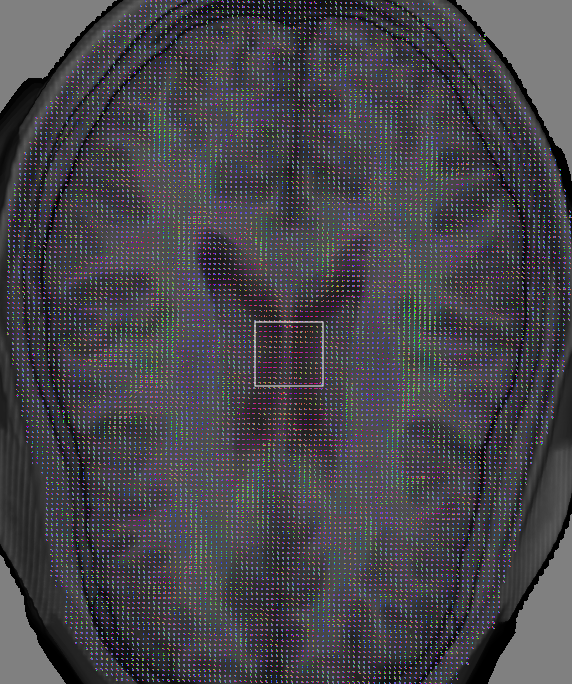
\includegraphics[width=.56\linewidth, angle=0]{figs/Esquema_Glifo/Teste_transicao/base_teste_zoom.png}
    \caption{MRI T1 anatômico co-registrado com DWI. A região dentro do contorno quadrado branco corresponde a região analisada na Fig. \ref{fig::multimodal_teste_zoom}.}
    \label{fig::multimodal_teste_loc}
\end{figure}


\begin{figure}[ht]
\centering
\captionsetup[subfloat]{farskip=0pt,nearskip=0pt}
    \subfloat[$4^a$ ordem de tesselação - apenas contornos dos triângulos]{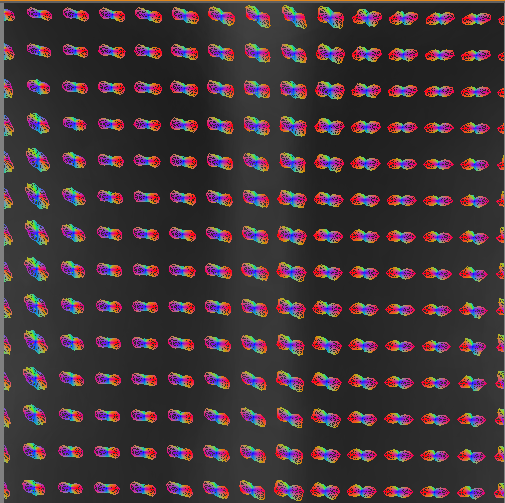
\includegraphics[width=.49\linewidth, angle=0]{figs/Esquema_Glifo/Teste_transicao/162_Hollow.png}
    \label{fig::multimodal_162_hollow}
    }
    \subfloat[$4^a$ ordem de tesselação - triângulos preenchidos] {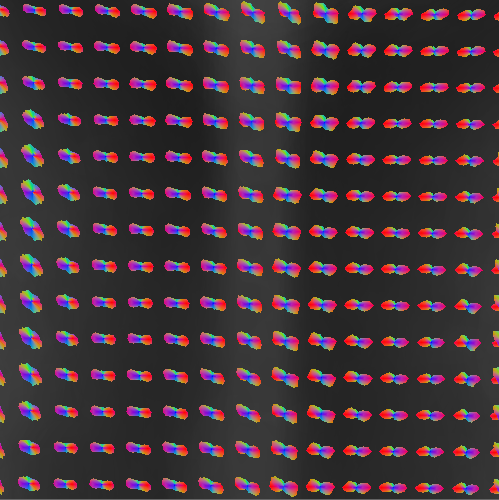
\includegraphics[width=.485\linewidth, angle=0]{figs/Esquema_Glifo/Teste_transicao/162_filled.png}
    \label{fig::multimodal_162_filled}
    }
    \hspace{1pt}
    \subfloat[$8^a$ ordem de tesselação - apenas contornos dos triângulos]{\includegraphics[width=.495\linewidth, angle=0]{figs/Esquema_Glifo/Teste_transicao/642_Hollow.png}
    \label{fig::multimodal_642_hollow}
    }
    \subfloat[$8^a$ ordem de tesselação - triângulos preenchidos] {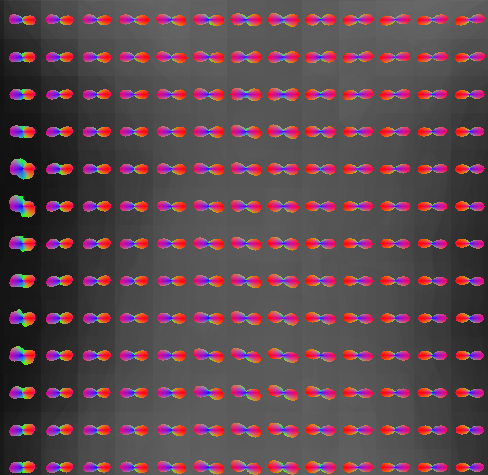
\includegraphics[width=.487\linewidth, angle=0]{figs/Esquema_Glifo/Teste_transicao/642_filled.png}
    \label{fig::multimodal_642_filled}
    }
    \caption{Ilustração da troca de resolução efetuada automaticamente a partir de $max_p$. A troca de resolução ocorre entre as geometrias base derivadas da $4^a$ (\ref{fig::multimodal_162_hollow} e \ref{fig::multimodal_162_filled}) e $8^a$ (\ref{fig::multimodal_642_hollow} e \ref{fig::multimodal_642_filled}) ordem de tesselação. A região ilustrada é do corpo caloso, que está em destaque na Fig. \ref{fig::multimodal_teste_loc}.
    }
    \label{fig::multimodal_teste_zoom}
\end{figure}

Podemos observar a suavidade em que a mudança de resolução ocorre. Observamos que os glifos com os triângulos preenchidos neste nível de resolução não apresentam efeitos característicos de malhas de baixa resolução e que a transição na resolução ocorre de forma sutil.

Adicionalmente, caso o usuário queira analisar os glifos mais de perto ou aumente o tamanho da janela, fazendo-a cobrir mais \textit{pixels}, o glifo é gerado a partir de uma malha suave o suficiente no qual ele tenha total liberdade para visualizar o comportamento das ODFs. Caso o usuário queira ter uma visão mais geral do volume com os glifos e diminua o fator de escala, diminuímos a resolução de cada glifo renderizado para aliviar o processamento computacional associado a cada um deles.


\subsubsection{Cruzamentos de Fibras}

Fig. \ref{fig::multimodal} ilustra uma fatia coronal na região do \textit{centrum semiovale} com um triplo cruzamento de fibras correspondentes do corpo caloso, \textit{corona radiata} e o fascículo longitudinal superior. A região apresenta cruzamentos de fibra conhecidos e é utilizada para análises qualitativas. Fig. \ref{fig::multimodal_highres} mostra que pode-se inferir sobre cada cruzamento de fibra nas regiões mais alongadas da superfície do glifo. Observe também que a resolução do glifo é diferente na Fig. \ref{fig::multimodal_lowres} em comparação a \ref{fig::multimodal_highres} e sua seleção é feita de forma automática. No fundo, há a renderização da ressonância anatômica ponderada em T1 co-registrada.

\begin{figure}[ht]
\centering
\captionsetup[subfloat]{farskip=0pt,nearskip=0pt}
    \subfloat[Fatia coronal de um MRI T1 co-registrado com DWI. A geometria base corresponde a $2^a$ ordem de tesselação do icosaedro.]{\makebox[1.2\width]{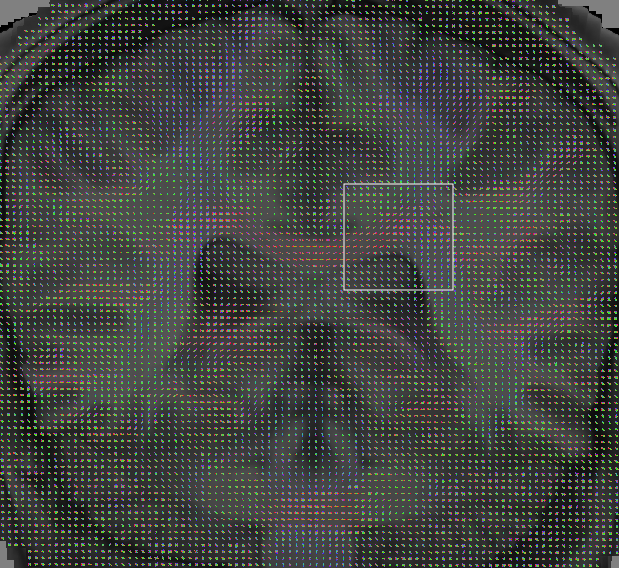
\includegraphics[width=.60\linewidth, angle=0]{figs/Esquema_Glifo/LowResImgHighlighted.png}}
    \label{fig::multimodal_lowres}
    }
    \hspace{1pt}
    
    \subfloat[Cruzamento entre fibras de corpo caloso (direita-esquerda), \textit{corona radiata} (descendente-ascendente) e fascículo longitudinal superior (anteroposterior - normal ao plano da página). A geometria base é a $8^a$ ordem de tesselação do icosaedro.] {\makebox[2.0\width]{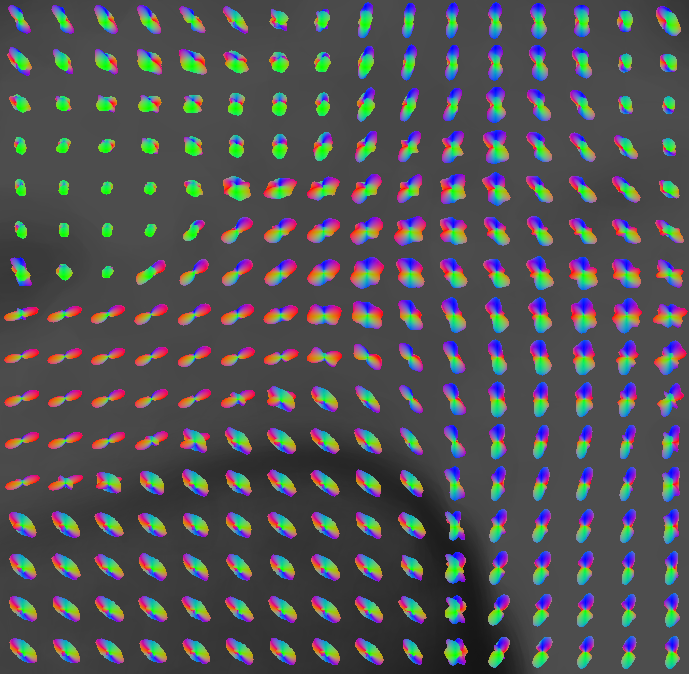
\includegraphics[width=.45\linewidth, angle=0]{figs/Esquema_Glifo/HighResImg.png}
    \label{fig::multimodal_highres}}
    }
    \caption{ Glifos ODF integrados ao ambiente de visualização multimodal para MRI. A imagem se refere a um MRI T1 cor-registrado a o seu respectivo DWI. \ref{fig::multimodal_highres} corresponde a região dentro do contorno de cor branca em \ref{fig::multimodal_lowres}.}
    \label{fig::multimodal}
\end{figure}



\citeonline{voltoline2021} evidenciaram que a sua respectiva renderização multimodal para superquádricas do DTI pode ajudar no processo de escolhas referentes a sementes em tractografia, em comparação à mapas de anisotropia codificados por cor. Fig. \ref{fig::multimodal_superquadric} ilustra a mesma região de Fig. \ref{fig::multimodal_highres} com superquádricas. Note que os glifos apresentam o mesmo problema presente no próprio DTI: em cruzamentos de fibra, a distribuição de fibras subjacente não é inferível. Pode-se perceber isto na região de cruzamento de fibras enquanto nos glifos ODF, é possível inferir sobre a natureza do cruzamento de fibras, nas superquádricas, o glifo apresenta uma forma retangular suave e não gera a possibilidade de inferir sobre as fibras que compõem o cruzamento.


\begin{figure}[ht]
    \centering
    %\rule{6cm}{3cm}
    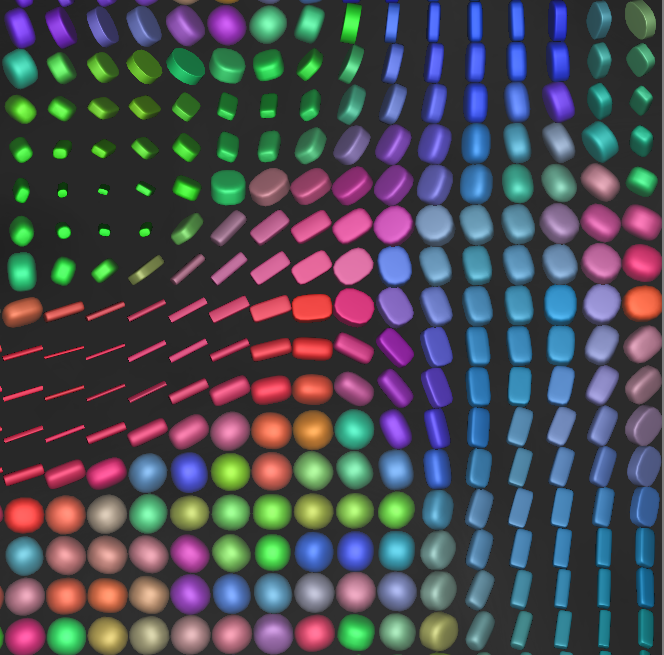
\includegraphics[width=.35\linewidth, angle=0]{figs/Esquema_Glifo/HighResImgSuperquadric.png}
    \caption{ Renderização multimodal para superquádricos do DTI. A imagem corresponde à mesma região em Fig. \ref{fig::multimodal_highres}.}
    \label{fig::multimodal_superquadric}
\end{figure}

\subsection{Performance}

Mensuramos o tempo de performance da renderização multimodal de glifos para ODF. O número de glifos é modificado pela mudança do fator de \textit{zoom}. Evidentemente que, maior o fator de \textit{zoom}, menor a quantidade de glifos, maior é a ocupância dos \textit{voxels} na tela, o que aumenta a resolução do glifos. A resolução da janela de saída é de $850\times 850$ e o número de glifos visíveis varia de 12 e 13360. A resolução dos glifos varia com a utilização de geometria base da $2^a$ ordem de tesselação do icosaedro (menor nível de detalhe, Fig. \ref{fig::multimodal_lowres}) até a $8^a$ (maior nível de detalhe, Fig. \ref{fig::multimodal_highres}). O FPS do esquema de renderização em função da quantidade de glifos renderizados e parâmetros relacionados de fator de escala e geometria base utilizados estão listados na Tabela \ref{tab::glyph_info_experiment}, onde atestamos que o esquema renderiza em taxas interativas \cite{nielsen1994}.



\begin{table}[]
\centering
\begin{tabular}{|cccc|}
\hline
\textbf{FPS} & \textbf{Fator de escala} & \textbf{\# glifos} & \textbf{\begin{tabular}[c]{@{}c@{}}Ordem de \\ tesselação\end{tabular}} \\ \hline
32.28 & 86.50 & 12     & 2³ \\
33.99 & 58.15 & 20     & 2³ \\
34.48 & 38.76 & 42     & 2³ \\
33.75 & 25.84 & 90     & 2³ \\
33.44 & 17.23 & 210    & 2³ \\
33.13 & 11.49 & 420    & 2³ \\
32.82 & 7.66  & 930    & 2² \\
34.73 & 5.10  & 2070   & 2² \\
31.19 & 3.40  & 4556   & 2² \\
21.58 & 2.27  & 9931   & 2² \\
17.92 & 1.51  & 13360  & 2  \\
\hline
\end{tabular}
\caption{Esquema de renderização multimodal com glifos de ODF renderizados em uma imagem $850\times 850$. O número de vértices e triângulos utilizados são computados de acordo com as Eq. \ref{eq::2ordem_icosphere_vertices} e \ref{eq::2ordem_icosphere_triangulos}.}
\label{tab::glyph_info_experiment}
\end{table}

\subsection{Renderização por Fatias}

Podemos comparar nossa abordagem com a de \citeonline{shattuck2008}, uma vez que ambas são baseadas em polígonos, onde amostras de ODF deformam uma malha esférica. Em sua abordagem, \citeonline{shattuck2008} armazena ODFs como coeficientes de funções base na CPU e os glifos são computados e visualizados em fatias, que são visualizadas de forma ortogonal. O cômputo da forma dos glifos é feito na CPU, onde o valor de ODF é computada para as normais dos vértices da malha esférica utilizada, deslocando cada um dos vértices, e o tráfego CPU-GPU consiste no envio de dados de vértices de forma que sua estrutura de dados define a superfície do glifo.

Em nossa abordagem, setamos a geometria base a priori e armazenamos amostras de dados de ODF e mostramos estratégias para escolher a geometria base adequada e estratégias para lidar com o gargalo de tráfego de dados CPU-GPU. Para atingir este objetivo, mostramos formas de organizar os dados de ODF e a da geometria base para utilizar renderização por instâncias, técnica que não estava disponível quando \citeonline{shattuck2008} publicaram seu trabalho\footnote{Em OpenGL, renderização por instâncias foi disponibilizada a partir da versão 3.2, lançada em 2009}. Adicionalmente, no processo de renderização, apenas enviamos um conjunto de escalares de ODF para deslocar a geometria base e deslocamos os pontos da malha nas \textit{threads} da GPU. Assim, o tráfego de dados por glifo é de $N/2 + (-N/2 \mod{4})$ floats para uma geometria base com $N$ vértices. A possibilidade de diminuir o tráfego de dados por glifo para esta quantidade tem sido crucial para renderizar este glifos com malhas suaves em taxas interativas. Adicionalmente, os glifos são renderizados com apenas um comando de desenho e sua quantidade máxima é limitada pelo máximo número de elementos permitidos em uma das dimensões da textura 2D.

Uma vez que nossa abordagem é vinculada à renderização de um volume com \textit{raycasting}, apenas os \textit{voxels} visíveis são requisitados a serem desenhados, e não há a restrição a uma fatia inteira. Além disso no ambiente interativo de visualização, onde o usuário tem a possibilidade de mudar a escala e mover o volume, a detecção de \textit{voxels} visíveis certifica que os \textit{voxels} que estão fora da cena não são demandados na renderização, consequentemente, seus dados não são enviados à GPU e nem são processados no \textit{vertex shader} para serem descartados na rasterização.

Nosso esquema é também aplicável em renderização de glifos baseada em fatia. Observe que, o conjunto $D$ pode se referir a um conjunto de índices referentes a \textit{voxels} que definem uma fatia. Adicionalmente, os atributos de translação podem posicionar os glifos em um \textit{grid} $W \times H$, onde este atributo posiciona cada objeto ao centro de cada célula, que é escalonado pelo fator que o faz estar contido.

Objetivando gerar resultados de performance do algoritmo e renderização em uma fatia 2-D, fizemos o seguinte experimento: os eixos x e y são divididos em $H$ intervalos ($W = H$), dando o total de $H^2$ células quadriculadas, no qual glifos são renderizados em cada uma delas. Cada glifo é escalonado para estar contido em sua respectiva célula e posicionado em seu centro. Fixamos a geometria base, assim como os atributos de translação e, para evidenciar a interatividade do algoritmo sob a circunstância de uma frequente troca de fatias, a cada requisição de desenho, os atributos de translação e a matriz de amostras de ODF são preparados e enviados à GPU, conforme mostrado na Subseção \ref{ssec::atributos}. Mensuramos o FPS como uma função da quantidade de glifos renderizados com $H$ variando de 5 até 100. O gráfico de $FPS \times \text{glifos renderizados}$ é ilustrado na Fig. \ref{fig::slice_benchmark} para diferentes geometria base utilizadas.

\begin{figure}[htb]
    \centering
    %\rule{6cm}{3cm}
    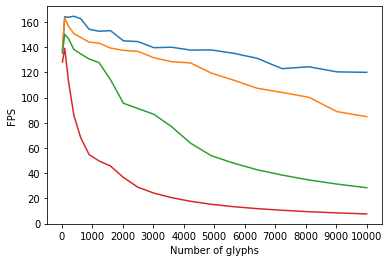
\includegraphics[width=.65\linewidth, angle=0]{figs/Esquema_Glifo/benchmark_half_texopt.png}
    \caption{FPS $\times$ quantidade de glifos renderizada. As cores azul, laranja, verde e vermelha correspondem a geometria base gerada pela $2^{a}$ $4^{a}$, $8^{a}$ e $16^{a}$ ordem de tesselação do icosaedro. Suas respectivas quantidades de vértices e triângulo são computadas nas Eq. \ref{eq::2ordem_icosphere_vertices} e \ref{eq::2ordem_icosphere_triangulos}, respectivamente.}
    \label{fig::slice_benchmark}
\end{figure}

Os resultados indicam que nosso esquema dá resultados satisfatórios para uso interativo, e mostramos que é possível renderizar milhares de glifos em taxas interativas utilizando a $4^{a}$ ordem de tesselação do icosaedro e centenas com a malha suave gerada pela $16^{a}$ ordem de tesselação.


%, no qual foi aperfeiçoado por \cite{almsick2011}. Esta abordagem possibilitou incrementos em performance em relação a \citeonline{shattuck2008}.

%\citeonline{raphael_dissertacao} propôs um esquema de renderização interativa do tensor de difusão em glifos superquádricos \cite{Kindlmann2004} utilizando polígonos. Em seu trabalho, os glifos são renderizados a taxas interativas e a sua abordagem consiste na minimização de tráfego de dados entre CPU-GPU, que consiste apenas em parâmetros que customizam e deslocam os glifos, e o uso de renderização por instâncias. Adicionalmente, este esquema está integrado ao VMTK-Neuro. Os resultados obtidos neste trabalho nos influenciou a adaptar o seu esquema para glifos HARDI.



%\subsection{\sout{Abordagem de renderização}}

%\sout{\citeonline{peeters2009} apresentou pela primeira vez um esquema de renderização para esta categoria de glifos, nos quais são aperfeiçoados por \citeonline{almsick2011} e \citeonline{hlawitschka2012}. Estes esquemas utilizam a abordagem \textit{raycasting}.}

%\sout{No VMTK-Neuro, um dos algoritmos de renderização do tensor difusão por glifos superquádricos é feita por instanciações de uma malha esférica, no qual é customizada por parâmetros particulares a cada tensor de difusão referentes a cada \textit{voxel} detectado e posicionado na cena de acordo. Este esquema de renderização desenha os glifos em tempo interativo.}

%\sout{Pela maior simplicidade e boa efetividade da renderização por instanciações de uma malha esférica, o esquema desenvolvido neste trabalho utiliza esta abordagem.}



%Dados relativos ao desempenho \sout{serão mais detalhados na dissertação de mestrado}\textcolor{blue}{estão disponíveis no link ...}.



%\sout{Medições do tempo relativo ao desempenho foram feitas para a quantidade de 197 vértices da malha esférica \sout{em um}\textcolor{blue}{num} volume de resolução 128x128x90. Para uma quantidade na faixa de 5000 glifos renderizados simultaneamente sobre uma fatia completa, obtemos tem um tempo de resposta entre 80 e 110ms. Para uma quantidade pequena de glifos na faixa das dezenas, o tempo de resposta cai para o intervalo entre 60 e 70ms. Esse tempo de resposta está nas proximidades ou é menor do que o tempo de 0,1s, que é o limite máximo para que o usuário tenha a percepção de resposta instantânea da máquina e que suas ações são a causa de que algo aconteça na tela \cite{nielsen1994}.}

%\sout{No cômputo das ODFs do \textit{QBall}, é feito o mapeamento do sinal de DWI para a ODF a partir das direções derivadas da malha esférica. O glifo para visualização é gerado diretamente de acordo a representação gráfica polar esférica em que $R(\textbf{u}) = \psi(\mathbf{u})$, onde \textbf{u} é a direção de difusão. A malha esférica utilizada para geração dos glifos em \ref{section::QBall_Glifos} está representada na figura \ref{fig::MalhaEsferico}.}

%A priori, todas as ODFs são calculadas e normalizadas para o intervalo $[0,1]$ para cada um dos \textit{voxels} do volume e referenciadas no processo de renderização.

%O formato de armazenamento dos valores ODF associados à malha consiste numa lista de valores escalares associados a cada um dos \textit{voxels}.



%\todo[inline]{Falta uma descrição melhor de como são construídos os glifos a partir de ODFs e o seu mapeamento às entidades gráficas. Isso torna difícil o entendimento da sua implementação. !!Descrito em trabalhos relacionados!}


\chapter{Conclusão}
\label{chap::conclusao}


Neste trabalho abordamos a visualização multimodal de imagens DWI com a utilização de um método para volumes de difusão com alta resolução angular junto com volumes escalares de outras modalidades, que está em desenvolvimento pelo nosso grupo de pesquisa \cite{VMTKNeuro}. Para alcançar este objetivo, implementamos o cômputo da amostragem generalizada no espaço-Q e implementamos a visualização das ODFs obtidas através do método, aproveitando a infraestrutura e funcionalidades implementadas de co-registro entre dois volumes \cite{ting2014} e a infraestrutura para renderização multimodal para DTI e glifos superquádricos \cite{voltoline2021}.

Para estimação de ODFs de difusão, implementamos o cômputo do método de imageamento amostragem generalizada no espaço-Q de acordo com o sugerido por \citeonline{yeh2010}. Derivamos o método até chegarmos em uma formulação que relaciona o sinal e o perfil de difusão em uma ODF através de uma multiplicação matricial. Armazenamos as ODFs em amostras e exploramos a sua simetria para armazenarmos ODFs de direções simétricas em um somente um valor.

Afim de prover um ambiente que se propõe a ser utilizado para avaliação de ODFs, desenvolvemos um algoritmo de renderização de ODFs em glifos, nos quais são posicionados em seus respectivos \textit{voxels} na renderização multimodal. Nos baseamos no algoritmo de renderização multimodal para volumes de ressonância magnética DWI e T1 co-registrados com glifos superquádricos proposto por \citeonline{voltoline2021} e utilizamos recursos modernos de GPU e técnicas modernas para renderizar os glifos em tempo interativo.

Para este fim, propomos maneiras de lidar com o alto tráfego de dados entre CPU-GPU relativo aos dados de ODF e para isso exploramos a percepção visual humana, e simetria das ODFs. Levando estes pontos em consideração, propomos uma forma de estruturar dados de amostras de ODF armazenadas na CPU. Adicionalmente, mostramos como os dados são enviados e acessados na GPU para gerar cada um dos glifos e como utilizamos a renderização por instanciação para gerá-los com um comando de desenho.

Nos experimentos que fizemos, atestamos que o algoritmo integrado ao ambiente de visualização multimodal renderiza quadros a uma taxa interativa e também mostramos que, através deles, é possível inferir acerca de cruzamentos de fibras.

\section{Futuros Trabalhos}

Para futuros trabalhos, podemos pesquisar o cômputo da distribuição local de fibras subjacentes às ODFs, bem como pesquisar e desenvolver uma abordagem de tractografia para gerar tratos do cérebro baseados na distribuição local, como mostrado no fluxograma da Fig. \ref{fig::flowchart_vmtk_hardi}. Podemos explorar o algoritmo de \citeonline{Chamberland2016}, que propôs um algoritmo onde as fibras são reconstruídas em tempo interativo a partir de distribuição local de fibras subjacentes pré-computadas e que entram de acordo com a visualização interativa proposta no VMTK-Neuro. Ressaltamos que métodos de tractografia baseadas em ODFs é um problema em aberto e alguns dos desafios da área podem ser encontrados em \citeonline{SCHILLING2019194}.

Por questões de otimização no uso de memória, que é muito demandada por ODFs de métodos HARDI, destacamos que é importante que haja uma forma de segmentar o cérebro para o volume de difusão, para que as amostras de ODF não sejam computadas e alocadas na memória para \textit{voxels} que não estão contidos no cérebro.

Na renderização multimodal para glifos ODF, podemos investigar a adaptação do algoritmo de renderização de glifos para ODFs que estejam representadas como funções base harmônicas esféricas, que são frequentemente utilizadas na comunidade HARDI \cite{descoteaux2007_QBI, Tournier2004DirectEO}.


%bem como desenvolver aplicações de visualização associadas. Adaptando muito do que já fora desenvolvido para o DTI, as aplicações desenvolvidas para o método consistem na estimação de ODFs via transformada de Funk-Radon, visualização em tempo interativo de ODFs em glifos e o desenvolvimento de um algoritmo de tractografia associado.

%Objetivando prover um ambiente que permite a avaliação de ODFs, aproveitando as funcionalidades presentes no VMTK-Neuro para exploração de DWIs e MRI anatômicos, foi desenvolvido um esquema de renderização em tempo interativo que mapeia as ODFs em suas representações gráficas polares esféricas.

%Com o objetivo de melhorar e tractografia baseada em DTI, foi implementado um protótipo de algoritmo de tractografia baseado em um conjunto de direções de métodos HARDI. !!(No trato corticoespinhal, no qual o DTI não consegue resolver).
%Adicionalmente, a tractografia gera resultados em tempo interativo para o usuário, permitindo-o explorar livremente para diferentes parâmetros.

%\section{Futuros trabalhos}

%Na renderização de glifos, pode-se implementar o cômputo de vetores normais para serem usados na iluminação das superfícies, o que é algo comum na apresentação por glifos. Adicionalmente, podemos implementar as representações polares esféricas sugerida por \citeonline{hlawitschka2012} e/ou \citeonline{almsick2011} para fins de comparação de performance com a nossa abordagem.

%Em tractografia, o próximo passo é a implementação do afiamento de ODFs, o que melhora extração de direções plausíveis de direções a serem usadas no \textit{tracking} de fibras \cite{fillard2011, SCHILLING2019194}.
\pagebreak
% \chapter{Apêndice}


% \section{Imagens de ODFs mapeadas em glifos renderizadas no VMTK-Neuro}

% \label{section::QBall_Glifos}

% \begin{figure}[H]
% \label{fig::QBall_glifos_axial}
% %\subfigcapskip = -5pt
%     \centering
%     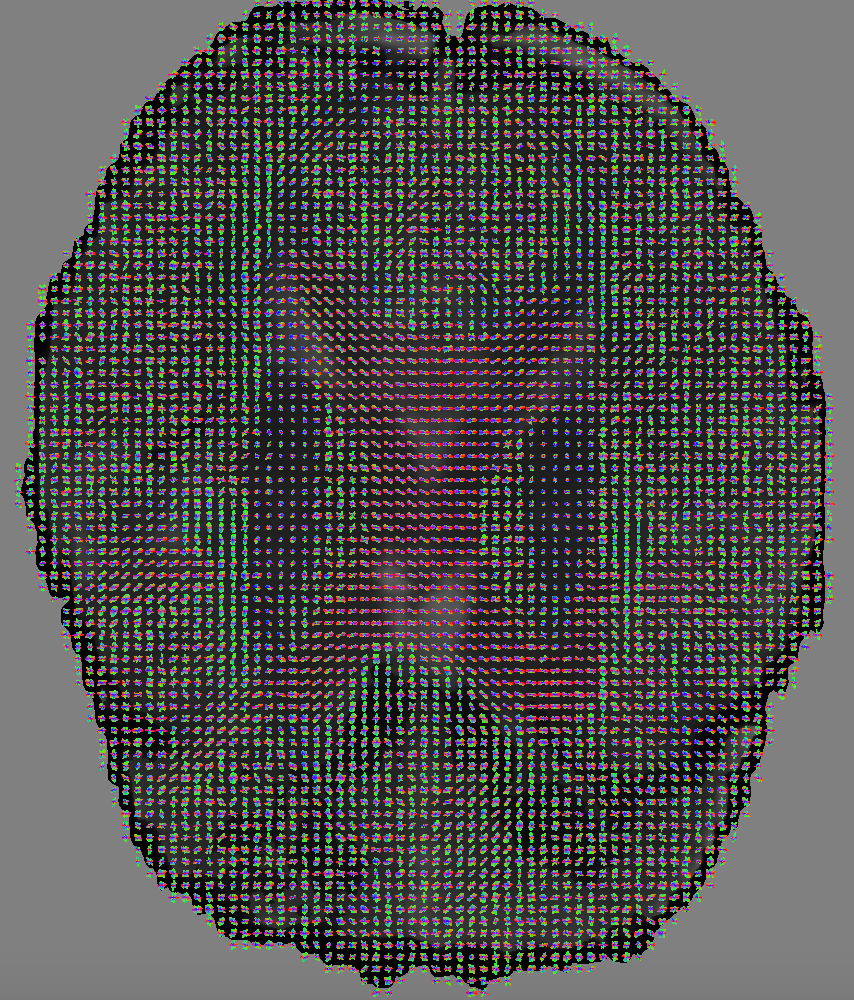
\includegraphics[width=1.0\linewidth, angle=0]{figs/Exemplos_QBall_visualizacao/Axial.png}
%      \caption{Projeção Axial.}
%  %   \hspace{1pt}
% \end{figure}

% \begin{figure}[H]
% \label{fig::QBall_glifos_sagital}
% %\subfigcapskip = -5pt
%     \centering

%     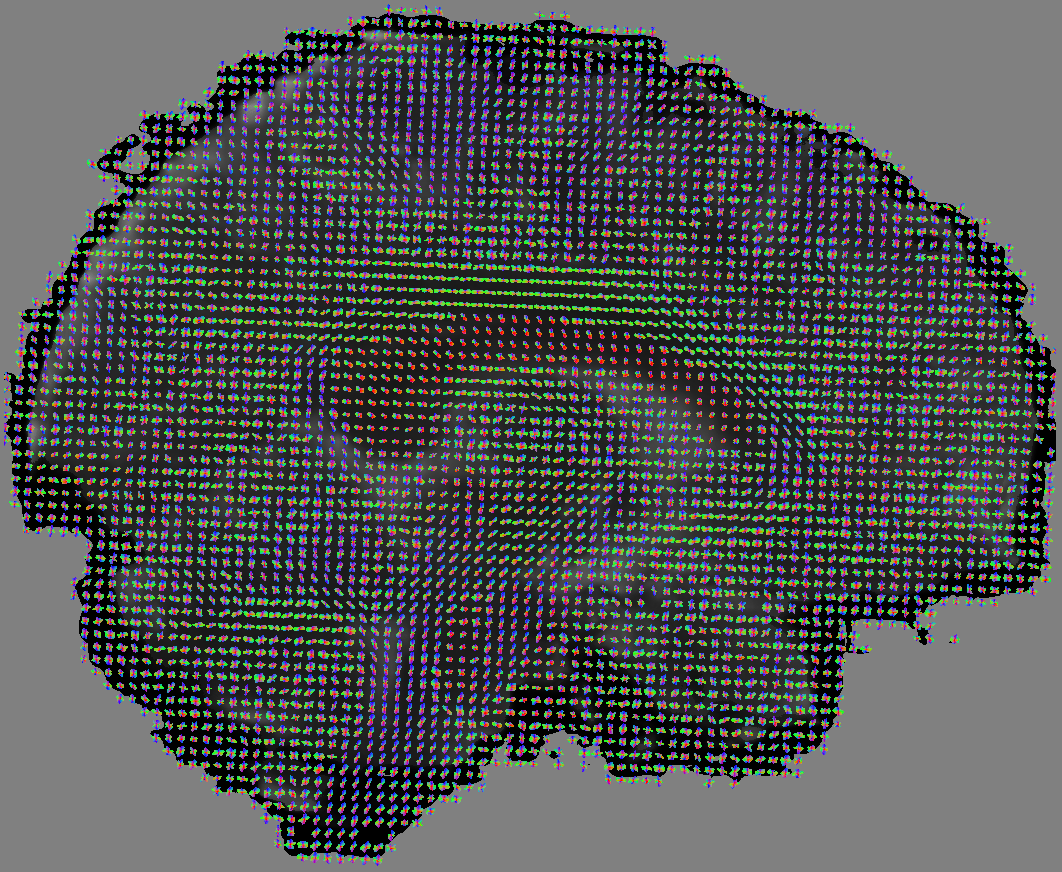
\includegraphics[width=.7\linewidth, angle=0]{figs/Exemplos_QBall_visualizacao/Sagital.png}
%     \caption{Projeção Sagital.}
%  %   \hspace{1pt}
% \end{figure}

% \begin{figure}[H]
% \label{fig::QBall_glifos_coronal}
% %\subfigcapskip = -5pt
%     \centering

%     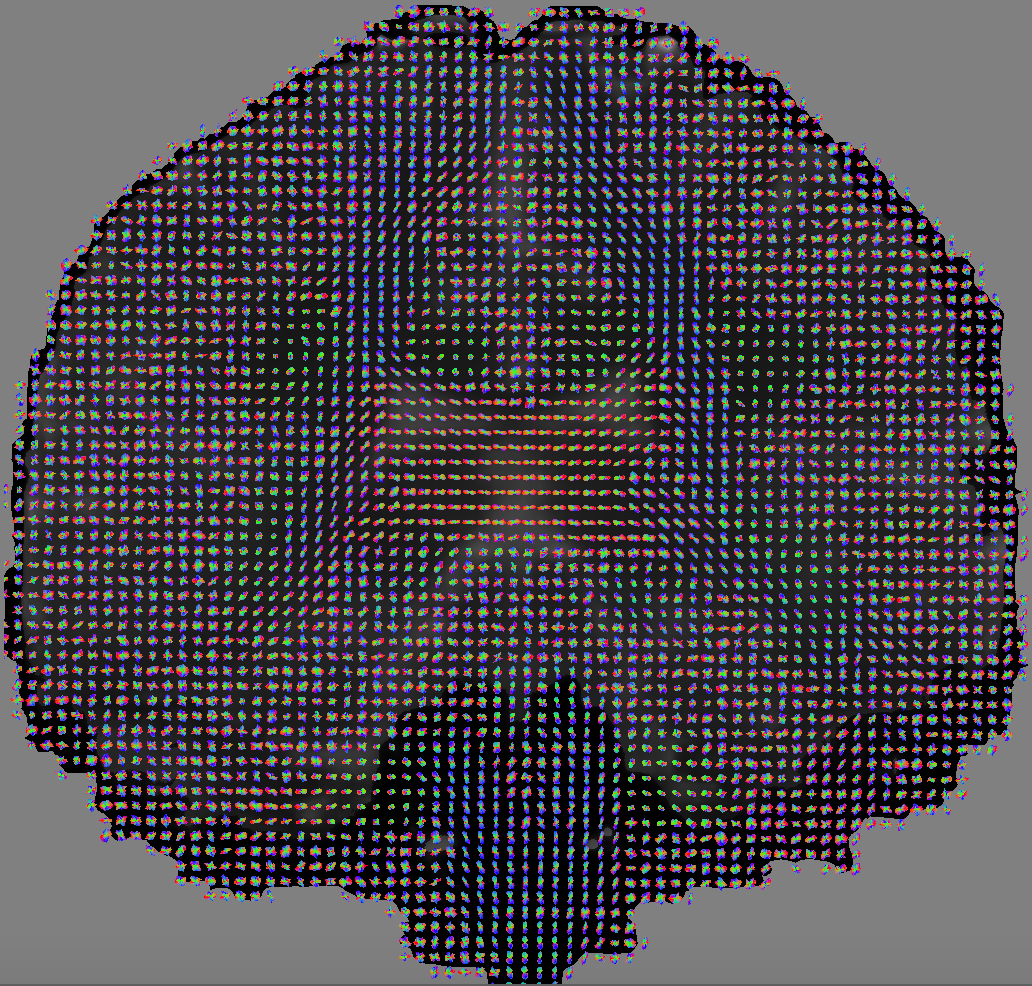
\includegraphics[width=0.7\linewidth, angle=0]{figs/Exemplos_QBall_visualizacao/Coronal.png}
%     \caption{Projeção Coronal.}
%  %   \hspace{1pt}
% \end{figure}

% \begin{figure}[H]
% \label{fig::QBall_glifos_Coronal_CC_CS}
% %\subfigcapskip = -5pt
%     \centering
%     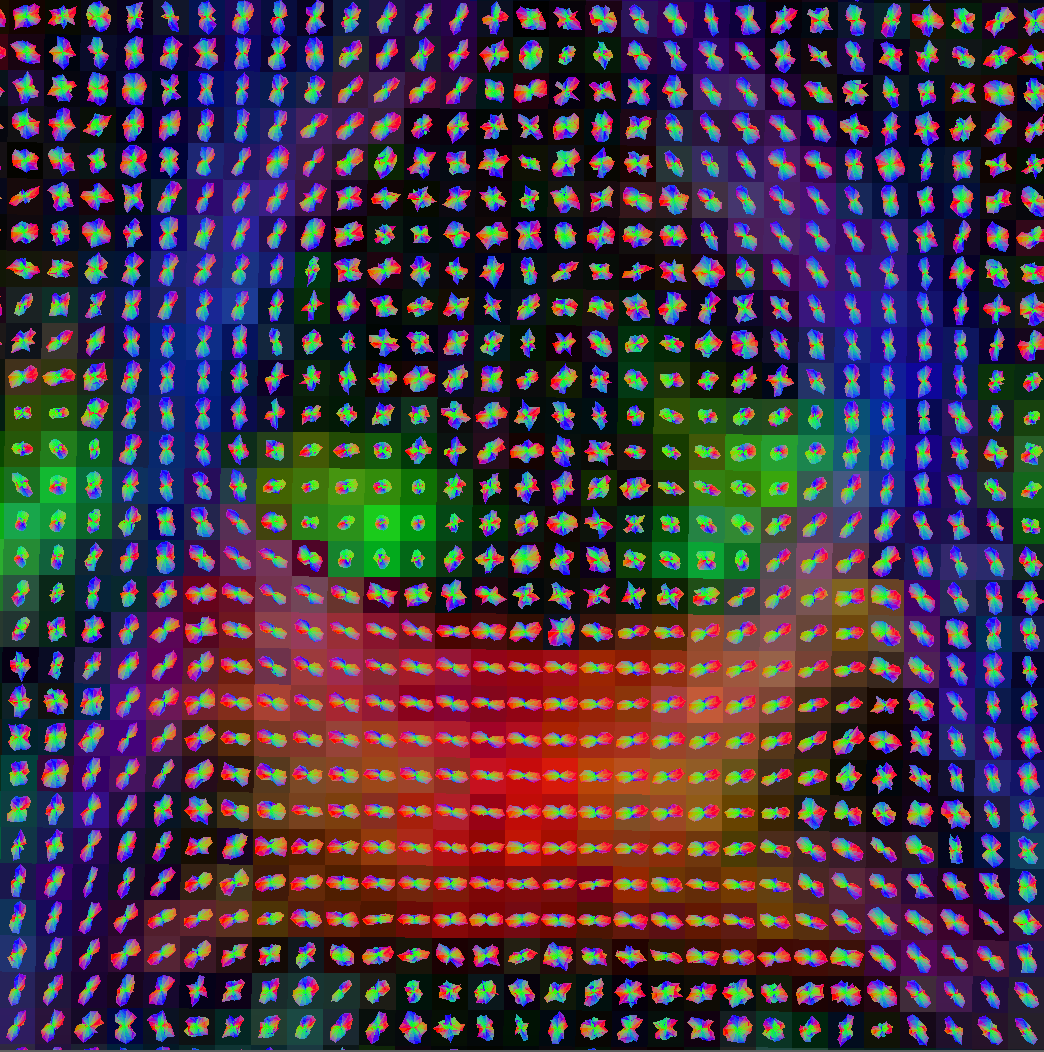
\includegraphics[width=.7\linewidth, angle=0]{figs/Exemplos_QBall_visualizacao/Coronal_Cruzamento_MapaFA.png}
%     \caption{Projeção Coronal - Região de cruzamento de fibras. Glifos renderizado sobre mapa FA codificado por cores do DTI.}
%  %   \hspace{1pt}
% \end{figure}

% \begin{figure}[H]
% \label{fig::QBall_glifos_azul}
% %\subfigcapskip = -5pt
%     \centering

%     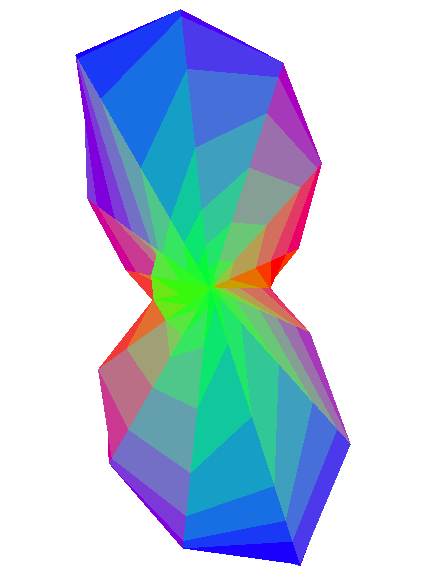
\includegraphics[width=.4\linewidth, angle=0]{figs/Exemplos_QBall_visualizacao/Glifo_Azul.png}
%     \caption{Glifo referente a um voxel com direção de difusão predominantemente ascendente.}
%  %   \hspace{1pt}
% \end{figure}

\pagebreak


\section{\textit{Overplus} e problemas com o mapeamento do sinal de difusão em ODFs}
\label{ssec::problema_overplus}

Após um estudo que visou comparar ODFs geradas a partir de diferentes esquemas de amostragem de gradientes de ponderação de difusão, concluímos que a falta de uniformidade do conjunto de gradientes do \textit{Overplus} no domínio esférico compromete a interpolação de sinais de difusão no processo de cômputo do \textit{Q-Ball}. A figura \ref{fig::shell_Overplus_VS_ISMRM} mostra a distribuição no \textit{shell}\footnote{\textit{Shell} é um consiste em um conjunto definido em uma esfera.} das direções dos gradientes do \textit{Overplus}, em adição ao utilizado no volume ISMRM 2015.

\begin{figure}[ht]
\centering
\captionsetup[subfloat]{farskip=5pt,nearskip=0pt}
    %!!VER SE ISSO TA CERTO
    \subfloat[\textit{Overplus}.] {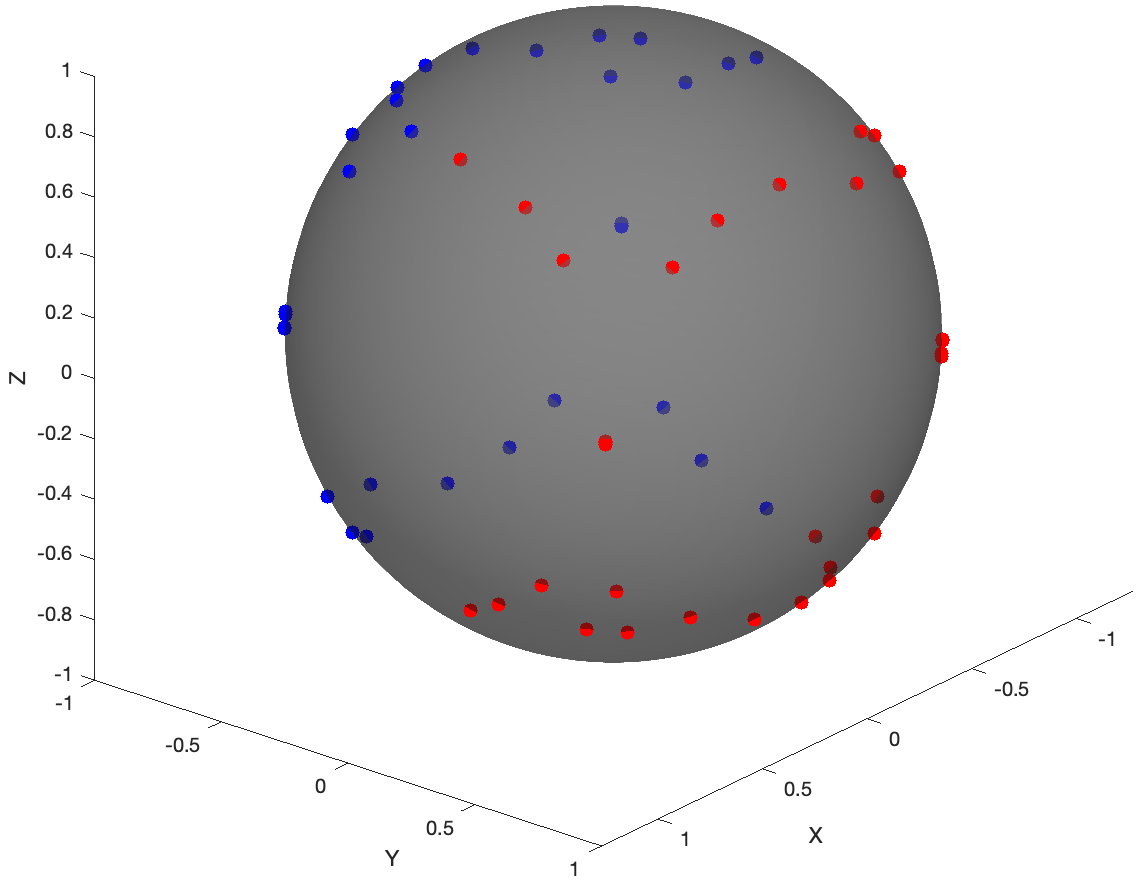
\includegraphics[width=.4\linewidth, angle=0]{figs/Overplus_VS_ISMRM/shell_overplus.png}}    
    \hfill
    \subfloat[Esquema utilizado no ISMRM.]{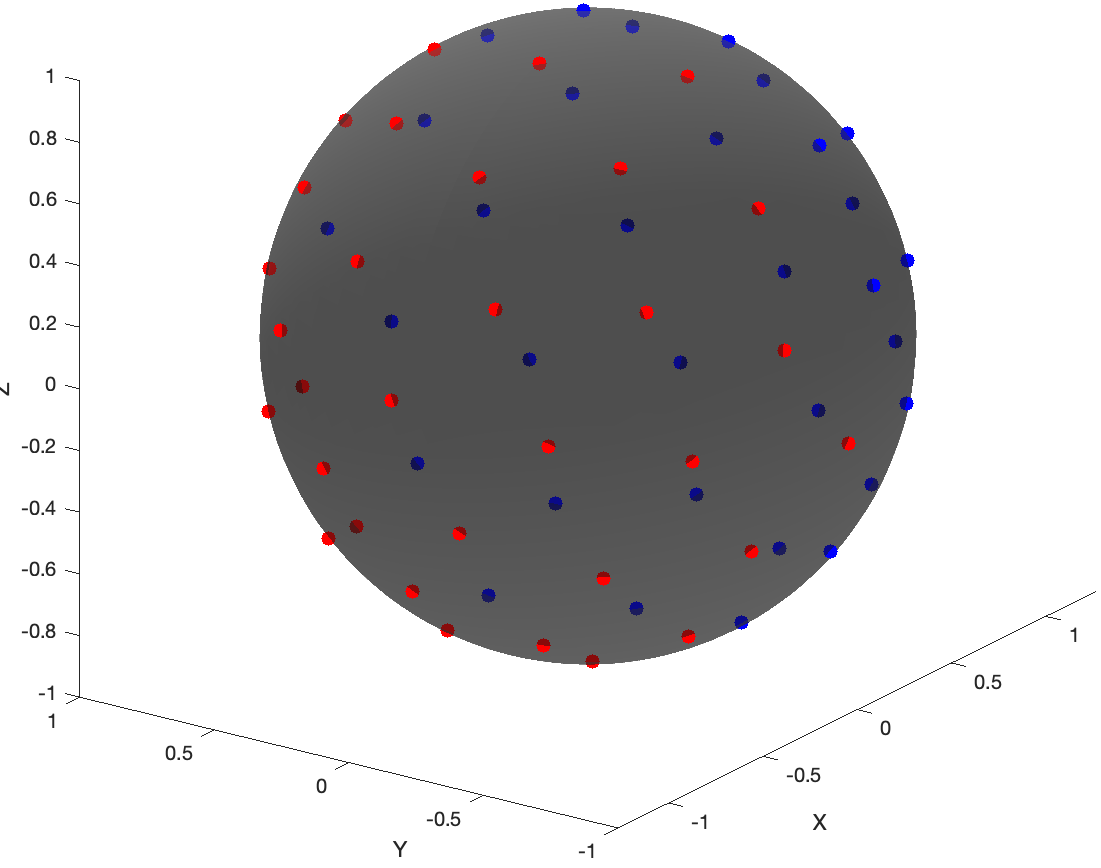
\includegraphics[width=.4\linewidth, angle=0]{figs/Overplus_VS_ISMRM/shell_ismrm.png}}
     \caption{Domínio esférico com pontos de amostragem referentes a direção de gradientes de difusão. Vermelho: direções de amostragem. Azul: sentido oposto da direção de amostragem.}
    %\hfill
    \label{fig::shell_Overplus_VS_ISMRM}
\end{figure}


Um bom conjunto de gradientes de codificação de difusão vinculada a um DWI não tem uma preferência direcional, as amostras no domínio esférico possuem uma boa invariância à orientação das estruturas do tecido ou coordenadas da máquina e a separação angular entre um par de pontos mais próximos é máxima e constante para todos os elementos \cite{cheng2018}. Um conjunto que segue essas propriedades estão distribuídos uniformemente sobre o \textit{shell}.

Há uma certa concordância na literatura de que uma uniformidade no domínio esférico em aquisições \textit{single shell}\footnote{Denomina-se aquisição \textit{single shell} como volumes de ressonância de difusão escaneados com apenas um valor b, além do b0.} é importante para uma boa reconstrução de ODFs. \citeonline{yeh2010} mencionam a importância da uniformidade além de propor uma métrica para aferir o seu grau. \citeonline{cheng2018} discorrem sobre formulações de esquemas de amostragem de gradientes de forma uniforme e mencionam as suas vantagens.

Como parte do processo de investigação dos resultados não esperados de ODFs gerados a partir dos volumes adquiridos através do protocolo \textit{Overplus}, foram escaneados para um mesmo indivíduo um volume com o conjunto de direções da competição ISMRM, o padrão, e um usando o protocolo \textit{Overplus} da Philips, em que todos possuem a mesma resolução angular de 32 direções. A análise feita consistiu na inspeção da forma dos glifos na região do corpo caloso que contém uma forte componente na direção mediolateral. A localização desta região se dá através do mapa FA codificado por cor gerado pelo DTI, em que não foi constatado nenhum problema nestes esquemas de aquisição.


Nesta inspeção, foi possível gerar glifos das ODFs razoáveis para o esquema de amostragem do ISMRM (Figura \ref{fig::Overplus_VS_ISMRM_b}), o que não aconteceu com o \textit{Overplus}, em que as ODFs ficaram totalmente descaracterizadas em comparação com os códigos de cores, conforme mostrado na Figura \ref{fig::Overplus_VS_ISMRM_a}.

\begin{figure}[ht]
\centering
\captionsetup[subfloat]{farskip=5pt,nearskip=0pt}
    
    \subfloat[\textit{Overplus}] {\label{fig::Overplus_VS_ISMRM_a} 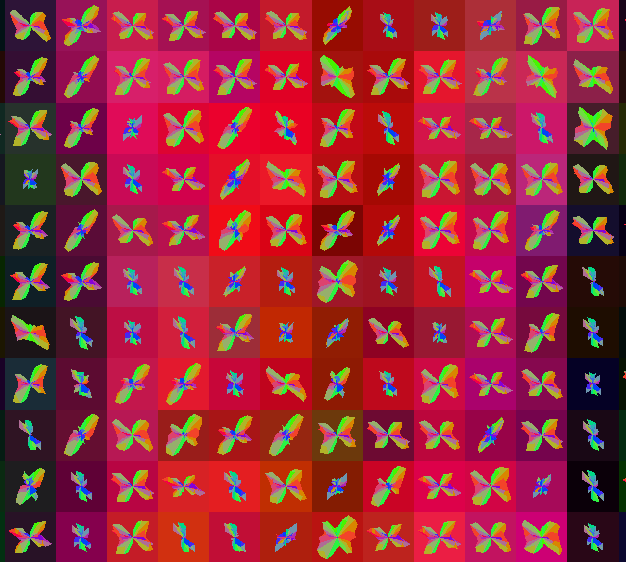
\includegraphics[width=.45\linewidth, angle=0, ]{figs/Overplus_VS_ISMRM/Overplus.png}}
    \hfill
    \subfloat[Esquema da competição ISMRM]{\label{fig::Overplus_VS_ISMRM_b} 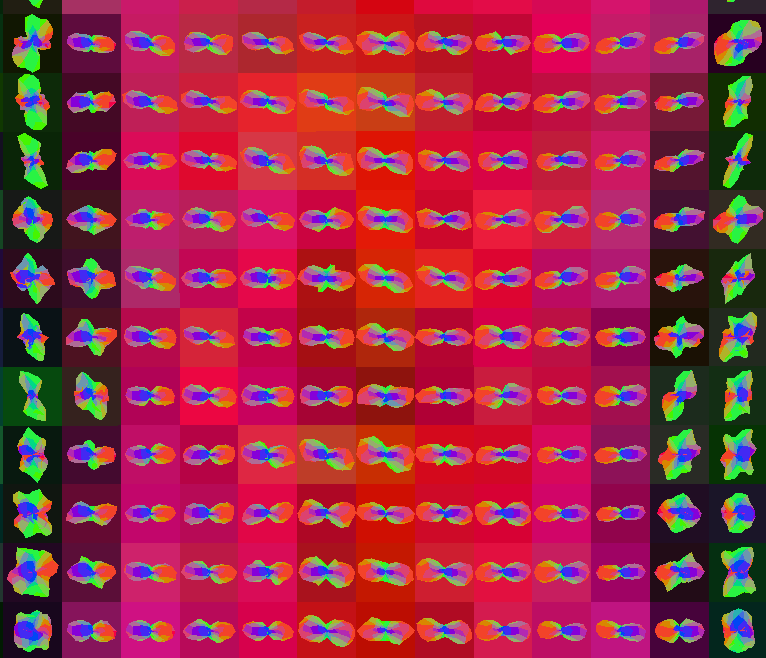
\includegraphics[width=.47\linewidth, angle=0]{figs/Overplus_VS_ISMRM/ISMRM.png}}
    %\hfill
    \caption{Glifos do Corpo Caloso - Mediolateral. Glifos de ODF sobre mapa FA codificado por cor do DTI.} %!!VER SE ISSO TA CERTO
    \label{fig::Overplus_VS_ISMRM}
\end{figure}
\pagebreak


%\bibliographystyle{}
\bibliography{references.bib}

% ----------------------------------------------------------
% Glossário
% ----------------------------------------------------------
%
% Consulte o manual da classe abntex2 para orientações sobre o glossário.
%
%\glossary

% ----------------------------------------------------------
% Apêndices
% ----------------------------------------------------------

% ---
% Inicia os apêndices
% ---
%\begin{apendicesenv}
%\end{apendicesenv}
% ---


% ----------------------------------------------------------
% Anexos
% ----------------------------------------------------------

% ---
% Inicia os anexos
% ---
\begin{anexosenv}
\end{anexosenv}

%---------------------------------------------------------------------
% INDICE REMISSIVO
%---------------------------------------------------------------------
%\phantompart
\printindex
%---------------------------------------------------------------------

\end{document}


